% Options for packages loaded elsewhere
\PassOptionsToPackage{unicode}{hyperref}
\PassOptionsToPackage{hyphens}{url}
\PassOptionsToPackage{dvipsnames,svgnames,x11names}{xcolor}
%
\documentclass[
  12pt,
  letterpaper,
  DIV=11,
  numbers=noendperiod]{scrartcl}

\usepackage{amsmath,amssymb}
\usepackage{setspace}
\usepackage{iftex}
\ifPDFTeX
  \usepackage[T1]{fontenc}
  \usepackage[utf8]{inputenc}
  \usepackage{textcomp} % provide euro and other symbols
\else % if luatex or xetex
  \usepackage{unicode-math}
  \defaultfontfeatures{Scale=MatchLowercase}
  \defaultfontfeatures[\rmfamily]{Ligatures=TeX,Scale=1}
\fi
\usepackage{lmodern}
\ifPDFTeX\else  
    % xetex/luatex font selection
\fi
% Use upquote if available, for straight quotes in verbatim environments
\IfFileExists{upquote.sty}{\usepackage{upquote}}{}
\IfFileExists{microtype.sty}{% use microtype if available
  \usepackage[]{microtype}
  \UseMicrotypeSet[protrusion]{basicmath} % disable protrusion for tt fonts
}{}
\makeatletter
\@ifundefined{KOMAClassName}{% if non-KOMA class
  \IfFileExists{parskip.sty}{%
    \usepackage{parskip}
  }{% else
    \setlength{\parindent}{0pt}
    \setlength{\parskip}{6pt plus 2pt minus 1pt}}
}{% if KOMA class
  \KOMAoptions{parskip=half}}
\makeatother
\usepackage{xcolor}
\usepackage[top=1.5cm,bottom=3cm,hmargin=2.5cm]{geometry}
\setlength{\emergencystretch}{3em} % prevent overfull lines
\setcounter{secnumdepth}{5}
% Make \paragraph and \subparagraph free-standing
\makeatletter
\ifx\paragraph\undefined\else
  \let\oldparagraph\paragraph
  \renewcommand{\paragraph}{
    \@ifstar
      \xxxParagraphStar
      \xxxParagraphNoStar
  }
  \newcommand{\xxxParagraphStar}[1]{\oldparagraph*{#1}\mbox{}}
  \newcommand{\xxxParagraphNoStar}[1]{\oldparagraph{#1}\mbox{}}
\fi
\ifx\subparagraph\undefined\else
  \let\oldsubparagraph\subparagraph
  \renewcommand{\subparagraph}{
    \@ifstar
      \xxxSubParagraphStar
      \xxxSubParagraphNoStar
  }
  \newcommand{\xxxSubParagraphStar}[1]{\oldsubparagraph*{#1}\mbox{}}
  \newcommand{\xxxSubParagraphNoStar}[1]{\oldsubparagraph{#1}\mbox{}}
\fi
\makeatother

\usepackage{color}
\usepackage{fancyvrb}
\newcommand{\VerbBar}{|}
\newcommand{\VERB}{\Verb[commandchars=\\\{\}]}
\DefineVerbatimEnvironment{Highlighting}{Verbatim}{commandchars=\\\{\}}
% Add ',fontsize=\small' for more characters per line
\usepackage{framed}
\definecolor{shadecolor}{RGB}{241,243,245}
\newenvironment{Shaded}{\begin{snugshade}}{\end{snugshade}}
\newcommand{\AlertTok}[1]{\textcolor[rgb]{0.68,0.00,0.00}{#1}}
\newcommand{\AnnotationTok}[1]{\textcolor[rgb]{0.37,0.37,0.37}{#1}}
\newcommand{\AttributeTok}[1]{\textcolor[rgb]{0.40,0.45,0.13}{#1}}
\newcommand{\BaseNTok}[1]{\textcolor[rgb]{0.68,0.00,0.00}{#1}}
\newcommand{\BuiltInTok}[1]{\textcolor[rgb]{0.00,0.23,0.31}{#1}}
\newcommand{\CharTok}[1]{\textcolor[rgb]{0.13,0.47,0.30}{#1}}
\newcommand{\CommentTok}[1]{\textcolor[rgb]{0.37,0.37,0.37}{#1}}
\newcommand{\CommentVarTok}[1]{\textcolor[rgb]{0.37,0.37,0.37}{\textit{#1}}}
\newcommand{\ConstantTok}[1]{\textcolor[rgb]{0.56,0.35,0.01}{#1}}
\newcommand{\ControlFlowTok}[1]{\textcolor[rgb]{0.00,0.23,0.31}{\textbf{#1}}}
\newcommand{\DataTypeTok}[1]{\textcolor[rgb]{0.68,0.00,0.00}{#1}}
\newcommand{\DecValTok}[1]{\textcolor[rgb]{0.68,0.00,0.00}{#1}}
\newcommand{\DocumentationTok}[1]{\textcolor[rgb]{0.37,0.37,0.37}{\textit{#1}}}
\newcommand{\ErrorTok}[1]{\textcolor[rgb]{0.68,0.00,0.00}{#1}}
\newcommand{\ExtensionTok}[1]{\textcolor[rgb]{0.00,0.23,0.31}{#1}}
\newcommand{\FloatTok}[1]{\textcolor[rgb]{0.68,0.00,0.00}{#1}}
\newcommand{\FunctionTok}[1]{\textcolor[rgb]{0.28,0.35,0.67}{#1}}
\newcommand{\ImportTok}[1]{\textcolor[rgb]{0.00,0.46,0.62}{#1}}
\newcommand{\InformationTok}[1]{\textcolor[rgb]{0.37,0.37,0.37}{#1}}
\newcommand{\KeywordTok}[1]{\textcolor[rgb]{0.00,0.23,0.31}{\textbf{#1}}}
\newcommand{\NormalTok}[1]{\textcolor[rgb]{0.00,0.23,0.31}{#1}}
\newcommand{\OperatorTok}[1]{\textcolor[rgb]{0.37,0.37,0.37}{#1}}
\newcommand{\OtherTok}[1]{\textcolor[rgb]{0.00,0.23,0.31}{#1}}
\newcommand{\PreprocessorTok}[1]{\textcolor[rgb]{0.68,0.00,0.00}{#1}}
\newcommand{\RegionMarkerTok}[1]{\textcolor[rgb]{0.00,0.23,0.31}{#1}}
\newcommand{\SpecialCharTok}[1]{\textcolor[rgb]{0.37,0.37,0.37}{#1}}
\newcommand{\SpecialStringTok}[1]{\textcolor[rgb]{0.13,0.47,0.30}{#1}}
\newcommand{\StringTok}[1]{\textcolor[rgb]{0.13,0.47,0.30}{#1}}
\newcommand{\VariableTok}[1]{\textcolor[rgb]{0.07,0.07,0.07}{#1}}
\newcommand{\VerbatimStringTok}[1]{\textcolor[rgb]{0.13,0.47,0.30}{#1}}
\newcommand{\WarningTok}[1]{\textcolor[rgb]{0.37,0.37,0.37}{\textit{#1}}}

\providecommand{\tightlist}{%
  \setlength{\itemsep}{0pt}\setlength{\parskip}{0pt}}\usepackage{longtable,booktabs,array}
\usepackage{calc} % for calculating minipage widths
% Correct order of tables after \paragraph or \subparagraph
\usepackage{etoolbox}
\makeatletter
\patchcmd\longtable{\par}{\if@noskipsec\mbox{}\fi\par}{}{}
\makeatother
% Allow footnotes in longtable head/foot
\IfFileExists{footnotehyper.sty}{\usepackage{footnotehyper}}{\usepackage{footnote}}
\makesavenoteenv{longtable}
\usepackage{graphicx}
\makeatletter
\newsavebox\pandoc@box
\newcommand*\pandocbounded[1]{% scales image to fit in text height/width
  \sbox\pandoc@box{#1}%
  \Gscale@div\@tempa{\textheight}{\dimexpr\ht\pandoc@box+\dp\pandoc@box\relax}%
  \Gscale@div\@tempb{\linewidth}{\wd\pandoc@box}%
  \ifdim\@tempb\p@<\@tempa\p@\let\@tempa\@tempb\fi% select the smaller of both
  \ifdim\@tempa\p@<\p@\scalebox{\@tempa}{\usebox\pandoc@box}%
  \else\usebox{\pandoc@box}%
  \fi%
}
% Set default figure placement to htbp
\def\fps@figure{htbp}
\makeatother

\usepackage{fvextra}
\DefineVerbatimEnvironment{Highlighting}{Verbatim}{
    commandchars=\\\{\},
    breaklines, breaknonspaceingroup, breakanywhere
}
\KOMAoption{captions}{tableheading}
\makeatletter
\@ifpackageloaded{caption}{}{\usepackage{caption}}
\AtBeginDocument{%
\ifdefined\contentsname
  \renewcommand*\contentsname{Table of contents}
\else
  \newcommand\contentsname{Table of contents}
\fi
\ifdefined\listfigurename
  \renewcommand*\listfigurename{List of Figures}
\else
  \newcommand\listfigurename{List of Figures}
\fi
\ifdefined\listtablename
  \renewcommand*\listtablename{List of Tables}
\else
  \newcommand\listtablename{List of Tables}
\fi
\ifdefined\figurename
  \renewcommand*\figurename{Figure}
\else
  \newcommand\figurename{Figure}
\fi
\ifdefined\tablename
  \renewcommand*\tablename{Table}
\else
  \newcommand\tablename{Table}
\fi
}
\@ifpackageloaded{float}{}{\usepackage{float}}
\floatstyle{ruled}
\@ifundefined{c@chapter}{\newfloat{codelisting}{h}{lop}}{\newfloat{codelisting}{h}{lop}[chapter]}
\floatname{codelisting}{Listing}
\newcommand*\listoflistings{\listof{codelisting}{List of Listings}}
\makeatother
\makeatletter
\makeatother
\makeatletter
\@ifpackageloaded{caption}{}{\usepackage{caption}}
\@ifpackageloaded{subcaption}{}{\usepackage{subcaption}}
\makeatother

\usepackage{bookmark}

\IfFileExists{xurl.sty}{\usepackage{xurl}}{} % add URL line breaks if available
\urlstyle{same} % disable monospaced font for URLs
\hypersetup{
  pdftitle={Detecting Bots on Reddit},
  pdfauthor={Matteo Mazzarelli},
  colorlinks=true,
  linkcolor={blue},
  filecolor={Maroon},
  citecolor={Blue},
  urlcolor={Blue},
  pdfcreator={LaTeX via pandoc}}


\title{Detecting Bots on Reddit}
\usepackage{etoolbox}
\makeatletter
\providecommand{\subtitle}[1]{% add subtitle to \maketitle
  \apptocmd{\@title}{\par {\large #1 \par}}{}{}
}
\makeatother
\subtitle{Computational Social Science}
\author{Matteo Mazzarelli}
\date{March 23, 2025}

\begin{document}
\maketitle


\setstretch{1}
\begin{Shaded}
\begin{Highlighting}[]
\ImportTok{import}\NormalTok{ base64}
\ImportTok{import}\NormalTok{ os}
\ImportTok{from}\NormalTok{ dotenv }\ImportTok{import}\NormalTok{ load\_dotenv }
\ImportTok{from}\NormalTok{ google }\ImportTok{import}\NormalTok{ genai}
\ImportTok{from}\NormalTok{ google.genai }\ImportTok{import}\NormalTok{ types}

\NormalTok{load\_dotenv()}

\CommentTok{\# set up LLM parameters}
\KeywordTok{def}\NormalTok{ generate(prompt):}
\NormalTok{    client }\OperatorTok{=}\NormalTok{ genai.Client(}
\NormalTok{        api\_key}\OperatorTok{=}\NormalTok{os.getenv(}\StringTok{"GEMINI\_API\_KEY"}\NormalTok{),}
\NormalTok{    )}

\NormalTok{    model }\OperatorTok{=} \StringTok{"gemini{-}2.0{-}flash"} \CommentTok{\# fastest model (used as default on the Gemini web app)}
\NormalTok{    contents }\OperatorTok{=}\NormalTok{ [}
\NormalTok{        types.Content(}
\NormalTok{            role}\OperatorTok{=}\StringTok{"user"}\NormalTok{,}
\NormalTok{            parts}\OperatorTok{=}\NormalTok{[}
\NormalTok{                types.Part.from\_text(text}\OperatorTok{=}\NormalTok{prompt),}
\NormalTok{            ],}
\NormalTok{        ),}
\NormalTok{    ]}
\NormalTok{    generate\_content\_config }\OperatorTok{=}\NormalTok{ types.GenerateContentConfig(}
\NormalTok{        temperature}\OperatorTok{=}\DecValTok{0}\NormalTok{, }\CommentTok{\# controls randomness. 0 = most deterministic (always selects highest probability token)}
\NormalTok{        top\_p}\OperatorTok{=}\DecValTok{0}\NormalTok{, }\CommentTok{\# nucleus sampling: limits token selection to the most probable. 0 = most deterministic (used when temperature \textgreater{} 0)}
\NormalTok{        top\_k}\OperatorTok{=}\DecValTok{1}\NormalTok{, }\CommentTok{\# restricts to top \textquotesingle{}k\textquotesingle{} tokens. 1 = most deterministic (used when temperature \textgreater{} 0)}
\NormalTok{        max\_output\_tokens}\OperatorTok{=}\DecValTok{8192}\NormalTok{,}
\NormalTok{        response\_mime\_type}\OperatorTok{=}\StringTok{"text/plain"}\NormalTok{,}
\NormalTok{    )}

\NormalTok{    complete\_response }\OperatorTok{=} \StringTok{""}
    \ControlFlowTok{for}\NormalTok{ chunk }\KeywordTok{in}\NormalTok{ client.models.generate\_content\_stream(}
\NormalTok{        model}\OperatorTok{=}\NormalTok{model,}
\NormalTok{        contents}\OperatorTok{=}\NormalTok{contents,}
\NormalTok{        config}\OperatorTok{=}\NormalTok{generate\_content\_config,}
\NormalTok{    ):}
\NormalTok{        complete\_response }\OperatorTok{+=}\NormalTok{ chunk.text}

    \ControlFlowTok{return}\NormalTok{ complete\_response}
\end{Highlighting}
\end{Shaded}

\begin{Shaded}
\begin{Highlighting}[]
\ImportTok{import}\NormalTok{ praw}
\ImportTok{import}\NormalTok{ pandas }\ImportTok{as}\NormalTok{ pd}

\CommentTok{\# Replace with your actual credentials}
\NormalTok{reddit }\OperatorTok{=}\NormalTok{ praw.Reddit(}
\NormalTok{    client\_id}\OperatorTok{=}\NormalTok{os.getenv(}\StringTok{"PRAW\_CLIENT\_ID"}\NormalTok{),}
\NormalTok{    client\_secret}\OperatorTok{=}\NormalTok{os.getenv(}\StringTok{"PRAW\_CLIENT\_SECRET"}\NormalTok{),}
\NormalTok{    user\_agent}\OperatorTok{=}\NormalTok{os.getenv(}\StringTok{"PRAW\_USER\_AGENT"}\NormalTok{),}
\NormalTok{    username}\OperatorTok{=}\NormalTok{os.getenv(}\StringTok{"PRAW\_USERNAME"}\NormalTok{),}
\NormalTok{    password}\OperatorTok{=}\NormalTok{os.getenv(}\StringTok{"PRAW\_PASSWORD"}\NormalTok{)}
\NormalTok{)}

\CommentTok{\# Fetch a large subset of popular subreddits (large limit makes this representative of the largest overall subreddits by subscribers, check: https://gummysearch.com/tools/top{-}subreddits/)}
\NormalTok{subreddits }\OperatorTok{=} \BuiltInTok{list}\NormalTok{(reddit.subreddits.popular(limit}\OperatorTok{=}\DecValTok{1000}\NormalTok{))}

\CommentTok{\# Create a DataFrame using list comprehension for better performance}
\NormalTok{subs\_df }\OperatorTok{=}\NormalTok{ pd.DataFrame([\{}
    \StringTok{"Name"}\NormalTok{: subreddit.display\_name,}
    \StringTok{"Subscribers"}\NormalTok{: subreddit.subscribers,}
    \StringTok{"Description"}\NormalTok{: subreddit.public\_description,}
    \StringTok{"Over 18"}\NormalTok{: subreddit.over18,}
    \StringTok{"Submission Type"}\NormalTok{: subreddit.submission\_type}
\NormalTok{\} }\ControlFlowTok{for}\NormalTok{ subreddit }\KeywordTok{in}\NormalTok{ subreddits]).sort\_values(by}\OperatorTok{=}\StringTok{"Subscribers"}\NormalTok{, ascending}\OperatorTok{=}\VariableTok{False}\NormalTok{, ignore\_index}\OperatorTok{=}\VariableTok{True}\NormalTok{)}

\CommentTok{\# Print the top 10}
\NormalTok{subs\_df.head(}\DecValTok{10}\NormalTok{)}
\end{Highlighting}
\end{Shaded}

\begin{longtable}[]{@{}llllll@{}}
\toprule\noalign{}
& Name & Subscribers & ... & Over 18 & Submission Type \\
\midrule\noalign{}
\endhead
\bottomrule\noalign{}
\endlastfoot
0 & funny & 66603813 & ... & False & any \\
1 & AskReddit & 53153687 & ... & False & self \\
2 & gaming & 46000086 & ... & False & any \\
3 & worldnews & 44840704 & ... & False & link \\
4 & todayilearned & 40121989 & ... & False & link \\
5 & aww & 37644769 & ... & False & link \\
6 & Music & 36986691 & ... & False & any \\
7 & memes & 35397379 & ... & False & link \\
8 & movies & 34847228 & ... & False & any \\
9 & Showerthoughts & 34152366 & ... & False & self \\
\end{longtable}

\begin{Shaded}
\begin{Highlighting}[]
\ImportTok{import}\NormalTok{ ast}

\NormalTok{response }\OperatorTok{=}\NormalTok{ generate(}\StringTok{"What are some keywords I can use to create a list of subreddits which are likely to be influenced by bots because of their controversial nature? These are keywords that I would look for within a subreddit\textquotesingle{}s name or description. For example: }\CharTok{\textbackslash{}"}\StringTok{news}\CharTok{\textbackslash{}"}\StringTok{, }\CharTok{\textbackslash{}"}\StringTok{politics}\CharTok{\textbackslash{}"}\StringTok{, }\CharTok{\textbackslash{}"}\StringTok{discussion}\CharTok{\textbackslash{}"}\StringTok{, }\CharTok{\textbackslash{}"}\StringTok{war}\CharTok{\textbackslash{}"}\StringTok{, }\CharTok{\textbackslash{}"}\StringTok{vaccines}\CharTok{\textbackslash{}"}\StringTok{, }\CharTok{\textbackslash{}"}\StringTok{controversial}\CharTok{\textbackslash{}"}\StringTok{, }\CharTok{\textbackslash{}"}\StringTok{conflict}\CharTok{\textbackslash{}"}\StringTok{, etc.}\CharTok{\textbackslash{}n\textbackslash{}n}\StringTok{Keep the answer short, only including 50 keywords and saving them in a python list as follows [}\CharTok{\textbackslash{}"}\StringTok{key1}\CharTok{\textbackslash{}"}\StringTok{,}\CharTok{\textbackslash{}"}\StringTok{key2}\CharTok{\textbackslash{}"}\StringTok{,...]. Send the output as text not as code."}\NormalTok{)}

\NormalTok{bot\_influence\_keywords }\OperatorTok{=}\NormalTok{ ast.literal\_eval(response.replace(}\StringTok{"}\CharTok{\textbackslash{}n}\StringTok{"}\NormalTok{, }\StringTok{""}\NormalTok{))}

\ControlFlowTok{for}\NormalTok{ i }\KeywordTok{in} \BuiltInTok{range}\NormalTok{(}\DecValTok{0}\NormalTok{, }\BuiltInTok{len}\NormalTok{(bot\_influence\_keywords), }\DecValTok{5}\NormalTok{):}
    \BuiltInTok{print}\NormalTok{(}\OperatorTok{*}\NormalTok{bot\_influence\_keywords[i:i}\OperatorTok{+}\DecValTok{5}\NormalTok{])}
\end{Highlighting}
\end{Shaded}

\begin{verbatim}
news politics discussion war vaccines
controversial conflict debate election government
rights freedom censorship truth conspiracy
agenda propaganda opinion ideology activism
resistance revolution socialism capitalism communism
nationalism globalism immigration border crime
justice police law gun religion
atheism gender race identity climate
energy economy finance markets technology
science health security military foreign policy
\end{verbatim}

\begin{Shaded}
\begin{Highlighting}[]
\CommentTok{\# Score subreddits based on subscribers and keywords in description}
\KeywordTok{def}\NormalTok{ calculate\_bot\_influence\_score(row):}
\NormalTok{    score }\OperatorTok{=} \DecValTok{0}
    
    \CommentTok{\# Large subscriber base increases potential for bot activity}
    \ControlFlowTok{if}\NormalTok{ row[}\StringTok{\textquotesingle{}Subscribers\textquotesingle{}}\NormalTok{] }\OperatorTok{\textgreater{}} \DecValTok{10000000}\NormalTok{:}
\NormalTok{        score }\OperatorTok{+=} \DecValTok{5}
    \ControlFlowTok{elif}\NormalTok{ row[}\StringTok{\textquotesingle{}Subscribers\textquotesingle{}}\NormalTok{] }\OperatorTok{\textgreater{}} \DecValTok{5000000}\NormalTok{:}
\NormalTok{        score }\OperatorTok{+=} \DecValTok{4}
    \ControlFlowTok{elif}\NormalTok{ row[}\StringTok{\textquotesingle{}Subscribers\textquotesingle{}}\NormalTok{] }\OperatorTok{\textgreater{}} \DecValTok{1000000}\NormalTok{:}
\NormalTok{        score }\OperatorTok{+=} \DecValTok{3}
        
    \CommentTok{\# Check for keywords in description and subreddit name}
\NormalTok{    description }\OperatorTok{=}\NormalTok{ row[}\StringTok{\textquotesingle{}Description\textquotesingle{}}\NormalTok{].lower()}
\NormalTok{    sub\_name }\OperatorTok{=}\NormalTok{ row[}\StringTok{\textquotesingle{}Name\textquotesingle{}}\NormalTok{].lower()}
    \ControlFlowTok{for}\NormalTok{ keyword }\KeywordTok{in}\NormalTok{ bot\_influence\_keywords:}
        \ControlFlowTok{if}\NormalTok{ keyword }\KeywordTok{in}\NormalTok{ description:}
\NormalTok{            score }\OperatorTok{+=} \DecValTok{1}
        \ControlFlowTok{if}\NormalTok{ keyword }\KeywordTok{in}\NormalTok{ sub\_name:}
\NormalTok{            score }\OperatorTok{+=} \DecValTok{1}
            
    \ControlFlowTok{return}\NormalTok{ score}

\NormalTok{subs\_df[}\StringTok{\textquotesingle{}Bot Score\textquotesingle{}}\NormalTok{] }\OperatorTok{=}\NormalTok{ subs\_df.}\BuiltInTok{apply}\NormalTok{(calculate\_bot\_influence\_score, axis}\OperatorTok{=}\DecValTok{1}\NormalTok{)}

\CommentTok{\# Get top 50 most vulnerable subreddits}
\NormalTok{top\_vulnerable }\OperatorTok{=}\NormalTok{ subs\_df.nlargest(}\DecValTok{50}\NormalTok{, }\StringTok{\textquotesingle{}Bot Score\textquotesingle{}}\NormalTok{)[[}\StringTok{\textquotesingle{}Name\textquotesingle{}}\NormalTok{, }\StringTok{\textquotesingle{}Subscribers\textquotesingle{}}\NormalTok{, }\StringTok{\textquotesingle{}Submission Type\textquotesingle{}}\NormalTok{, }\StringTok{\textquotesingle{}Bot Score\textquotesingle{}}\NormalTok{]].reset\_index(drop}\OperatorTok{=}\VariableTok{True}\NormalTok{)}
\NormalTok{top\_vulnerable.head(}\DecValTok{10}\NormalTok{)}
\end{Highlighting}
\end{Shaded}

\begin{longtable}[]{@{}lllll@{}}
\toprule\noalign{}
& Name & Subscribers & Submission Type & Bot Score \\
\midrule\noalign{}
\endhead
\bottomrule\noalign{}
\endlastfoot
0 & technology & 18515796 & link & 9 \\
1 & IndiaSpeaks & 1049165 & any & 9 \\
2 & pcmasterrace & 14761961 & any & 8 \\
3 & TwoXChromosomes & 13637547 & any & 8 \\
4 & politics & 8785009 & link & 8 \\
5 & worldnews & 44840704 & link & 7 \\
6 & movies & 34847228 & any & 7 \\
7 & science & 33802310 & link & 7 \\
8 & news & 29799417 & link & 7 \\
9 & askscience & 26054558 & self & 7 \\
\end{longtable}

\begin{Shaded}
\begin{Highlighting}[]
\CommentTok{\# Filter the DataFrame to include only the desired subreddits}
\NormalTok{subreddits\_of\_interest }\OperatorTok{=}\NormalTok{ [}\StringTok{\textquotesingle{}worldnews\textquotesingle{}}\NormalTok{, }\StringTok{\textquotesingle{}news\textquotesingle{}}\NormalTok{, }\StringTok{\textquotesingle{}politics\textquotesingle{}}\NormalTok{, }\StringTok{\textquotesingle{}science\textquotesingle{}}\NormalTok{, }\StringTok{\textquotesingle{}technology\textquotesingle{}}\NormalTok{]}
\NormalTok{top\_vulnerable\_filtered }\OperatorTok{=}\NormalTok{ top\_vulnerable[top\_vulnerable[}\StringTok{\textquotesingle{}Name\textquotesingle{}}\NormalTok{].isin(subreddits\_of\_interest)].reset\_index(drop}\OperatorTok{=}\VariableTok{True}\NormalTok{)}

\NormalTok{top\_vulnerable\_filtered}
\end{Highlighting}
\end{Shaded}

\begin{Shaded}
\begin{Highlighting}[]
\ImportTok{import}\NormalTok{ time}
\ImportTok{import}\NormalTok{ concurrent.futures}

\CommentTok{\# Function to Fetch Posts and Comments}
\KeywordTok{def}\NormalTok{ fetch\_posts\_and\_comments(subreddit\_name, num\_posts}\OperatorTok{=}\DecValTok{50}\NormalTok{, num\_comments}\OperatorTok{=}\DecValTok{2000}\NormalTok{):}
    \CommentTok{"""}
\CommentTok{    Fetches posts and their comments from a subreddit, including comment levels and parent comment ID.}

\CommentTok{    Args:}
\CommentTok{        subreddit\_name: The name of the subreddit.}
\CommentTok{        num\_posts: The maximum number of posts to fetch.}
\CommentTok{        num\_comments: The maximum number of comments to fetch per post (total, across all levels).}

\CommentTok{    Returns:}
\CommentTok{        A list of dictionaries, where each dictionary represents a post and its comments,}
\CommentTok{        with each comment including its level and parent comment ID.}
\CommentTok{    """}
\NormalTok{    subreddit }\OperatorTok{=}\NormalTok{ reddit.subreddit(subreddit\_name)}
\NormalTok{    posts\_data }\OperatorTok{=}\NormalTok{ []}

    \ControlFlowTok{try}\NormalTok{:}
        \ControlFlowTok{for}\NormalTok{ post }\KeywordTok{in}\NormalTok{ subreddit.hot(limit}\OperatorTok{=}\NormalTok{num\_posts):  }\CommentTok{\# You can change \textquotesingle{}hot\textquotesingle{} to \textquotesingle{}new\textquotesingle{}, \textquotesingle{}rising\textquotesingle{}, etc.}
\NormalTok{            post\_data }\OperatorTok{=}\NormalTok{ \{}
                \StringTok{"subreddit"}\NormalTok{: subreddit\_name,}
                \StringTok{"post\_id"}\NormalTok{: post.}\BuiltInTok{id}\NormalTok{,}
                \StringTok{"post\_title"}\NormalTok{: post.title,}
                \StringTok{"post\_author"}\NormalTok{: }\BuiltInTok{str}\NormalTok{(post.author),}
                \StringTok{"post\_score"}\NormalTok{: post.score,}
                \StringTok{"post\_upvote\_ratio"}\NormalTok{: post.upvote\_ratio,}
                \StringTok{"post\_url"}\NormalTok{: post.url,}
                \StringTok{"post\_selftext"}\NormalTok{: post.selftext,}
                \StringTok{"post\_created\_utc"}\NormalTok{: post.created\_utc,}
                \StringTok{"comments"}\NormalTok{: []}
\NormalTok{            \}}

            \KeywordTok{def}\NormalTok{ fetch\_comments\_recursive(comments, level}\OperatorTok{=}\DecValTok{1}\NormalTok{, comment\_count}\OperatorTok{=}\DecValTok{0}\NormalTok{, parent\_id}\OperatorTok{=}\VariableTok{None}\NormalTok{):}
\NormalTok{                comment\_data }\OperatorTok{=}\NormalTok{ []}
                \ControlFlowTok{for}\NormalTok{ comment }\KeywordTok{in}\NormalTok{ comments:}
                    \ControlFlowTok{if}\NormalTok{ comment\_count }\OperatorTok{\textgreater{}=}\NormalTok{ num\_comments:}
                        \ControlFlowTok{break}  \CommentTok{\# Stop fetching comments if the limit is reached}

\NormalTok{                    comment\_data.append(\{}
                        \StringTok{"comment\_id"}\NormalTok{: comment.}\BuiltInTok{id}\NormalTok{,}
                        \StringTok{"comment\_author"}\NormalTok{: }\BuiltInTok{str}\NormalTok{(comment.author),}
                        \StringTok{"comment\_body"}\NormalTok{: comment.body,}
                        \StringTok{"comment\_score"}\NormalTok{: comment.score,}
                        \StringTok{"comment\_created\_utc"}\NormalTok{: comment.created\_utc,}
                        \StringTok{"comment\_level"}\NormalTok{: level,  }\CommentTok{\# Add the comment level}
                        \StringTok{"parent\_id"}\NormalTok{: parent\_id  }\CommentTok{\# Add the parent comment ID}
\NormalTok{                    \})}
\NormalTok{                    comment\_count }\OperatorTok{+=} \DecValTok{1}

                    \CommentTok{\# Fetch replies recursively}
                    \ControlFlowTok{if} \BuiltInTok{hasattr}\NormalTok{(comment, }\StringTok{\textquotesingle{}replies\textquotesingle{}}\NormalTok{):}
\NormalTok{                        comment.replies.replace\_more(limit}\OperatorTok{=}\DecValTok{0}\NormalTok{)  }\CommentTok{\# Ensure all \textquotesingle{}MoreComments\textquotesingle{} are resolved}
\NormalTok{                        replies\_data, comment\_count }\OperatorTok{=}\NormalTok{ fetch\_comments\_recursive(comment.replies, level }\OperatorTok{+} \DecValTok{1}\NormalTok{, comment\_count, comment.}\BuiltInTok{id}\NormalTok{)}
\NormalTok{                        comment\_data.extend(replies\_data)}

                \ControlFlowTok{return}\NormalTok{ comment\_data, comment\_count}

\NormalTok{            post.comments.replace\_more(limit}\OperatorTok{=}\DecValTok{0}\NormalTok{)  }\CommentTok{\# Ensure all top{-}level \textquotesingle{}MoreComments\textquotesingle{} are resolved}
\NormalTok{            comments\_data, \_ }\OperatorTok{=}\NormalTok{ fetch\_comments\_recursive(post.comments)}
\NormalTok{            post\_data[}\StringTok{"comments"}\NormalTok{] }\OperatorTok{=}\NormalTok{ comments\_data}

\NormalTok{            posts\_data.append(post\_data)}

            \CommentTok{\# Respect API rate limits}
            \CommentTok{\# time.sleep(1)}

    \ControlFlowTok{except} \PreprocessorTok{Exception} \ImportTok{as}\NormalTok{ e:}
        \BuiltInTok{print}\NormalTok{(}\SpecialStringTok{f"Error fetching data from r/}\SpecialCharTok{\{}\NormalTok{subreddit\_name}\SpecialCharTok{\}}\SpecialStringTok{: }\SpecialCharTok{\{}\NormalTok{e}\SpecialCharTok{\}}\SpecialStringTok{"}\NormalTok{)}

    \ControlFlowTok{return}\NormalTok{ posts\_data}

\CommentTok{\# Main Data Collection Loop}
\NormalTok{all\_data }\OperatorTok{=}\NormalTok{ []}
\NormalTok{subreddit\_names }\OperatorTok{=}\NormalTok{ top\_vulnerable\_filtered[}\StringTok{\textquotesingle{}Name\textquotesingle{}}\NormalTok{].tolist()}
\NormalTok{num\_cores }\OperatorTok{=}\NormalTok{ os.cpu\_count()  }\CommentTok{\# Get the number of CPU cores}

\ControlFlowTok{with}\NormalTok{ concurrent.futures.ThreadPoolExecutor(max\_workers}\OperatorTok{=}\NormalTok{num\_cores) }\ImportTok{as}\NormalTok{ executor:}
    \CommentTok{\# Submit tasks to the executor}
\NormalTok{    futures }\OperatorTok{=}\NormalTok{ [executor.submit(fetch\_posts\_and\_comments, subreddit\_name, num\_posts}\OperatorTok{=}\DecValTok{50}\NormalTok{, num\_comments}\OperatorTok{=}\DecValTok{50}\NormalTok{) }\ControlFlowTok{for}\NormalTok{ subreddit\_name }\KeywordTok{in}\NormalTok{ subreddit\_names]}

    \CommentTok{\# Wait for all tasks to complete and collect results}
    \ControlFlowTok{for}\NormalTok{ future }\KeywordTok{in}\NormalTok{ concurrent.futures.as\_completed(futures):}
        \ControlFlowTok{try}\NormalTok{:}
\NormalTok{            subreddit\_data }\OperatorTok{=}\NormalTok{ future.result()}
\NormalTok{            all\_data.extend(subreddit\_data)}
        \ControlFlowTok{except} \PreprocessorTok{Exception} \ImportTok{as}\NormalTok{ e:}
            \BuiltInTok{print}\NormalTok{(}\SpecialStringTok{f"Error fetching data: }\SpecialCharTok{\{}\NormalTok{e}\SpecialCharTok{\}}\SpecialStringTok{"}\NormalTok{)}

\CommentTok{\# Convert to DataFrame}
\NormalTok{reddit\_data\_df }\OperatorTok{=}\NormalTok{ pd.DataFrame(all\_data)}

\CommentTok{\# Convert lists of comments to a separate DataFrame if desired}
\NormalTok{comments\_data }\OperatorTok{=}\NormalTok{ []}
\ControlFlowTok{for}\NormalTok{ index, row }\KeywordTok{in}\NormalTok{ reddit\_data\_df.iterrows():}
    \ControlFlowTok{for}\NormalTok{ comment }\KeywordTok{in}\NormalTok{ row[}\StringTok{\textquotesingle{}comments\textquotesingle{}}\NormalTok{]:}
\NormalTok{        comment[}\StringTok{\textquotesingle{}post\_id\textquotesingle{}}\NormalTok{] }\OperatorTok{=}\NormalTok{ row[}\StringTok{\textquotesingle{}post\_id\textquotesingle{}}\NormalTok{] }\CommentTok{\# add the relationship}
\NormalTok{        comments\_data.append(comment)}
\NormalTok{comments\_df }\OperatorTok{=}\NormalTok{ pd.DataFrame(comments\_data)}
\CommentTok{\# Expand the comments into its own columns}
\CommentTok{\# reddit\_data\_df = pd.concat([reddit\_data\_df.drop([\textquotesingle{}comments\textquotesingle{}], axis=1), pd.DataFrame(reddit\_data\_df[\textquotesingle{}comments\textquotesingle{}].tolist()).add\_prefix(\textquotesingle{}comment\_\textquotesingle{})], axis=1)}

\CommentTok{\# Export to CSV}
\NormalTok{reddit\_data\_df.to\_csv(}\StringTok{"reddit\_posts\_and\_comments.csv"}\NormalTok{, index}\OperatorTok{=}\VariableTok{False}\NormalTok{)}
\NormalTok{comments\_df.to\_csv(}\StringTok{"comments.csv"}\NormalTok{, index}\OperatorTok{=}\VariableTok{False}\NormalTok{)}
\end{Highlighting}
\end{Shaded}

\begin{Shaded}
\begin{Highlighting}[]
\ImportTok{import}\NormalTok{ pandas }\ImportTok{as}\NormalTok{ pd}

\NormalTok{reddit\_data\_df }\OperatorTok{=}\NormalTok{ pd.read\_csv(}\StringTok{"workspaces/reddit\_posts\_and\_comments\_03{-}21{-}1950.csv"}\NormalTok{)}

\NormalTok{reddit\_data\_df.head(}\DecValTok{10}\NormalTok{)}
\end{Highlighting}
\end{Shaded}

\begin{longtable}[]{@{}llllll@{}}
\toprule\noalign{}
& subreddit & post\_id & ... & post\_created\_utc & comments \\
\midrule\noalign{}
\endhead
\bottomrule\noalign{}
\endlastfoot
0 & science & 1jgfinq & ... & 1.742560e+09 &
{[}\{\textquotesingle comment\_id\textquotesingle:
\textquotesingle miyn7eg\textquotesingle,
\textquotesingle comment\_author\textquotesingle: \textquotesingle... \\
1 & science & 1jgl88s & ... & 1.742575e+09 &
{[}\{\textquotesingle comment\_id\textquotesingle:
\textquotesingle mj00hoq\textquotesingle,
\textquotesingle comment\_author\textquotesingle: \textquotesingle... \\
2 & science & 1jgerd9 & ... & 1.742557e+09 &
{[}\{\textquotesingle comment\_id\textquotesingle:
\textquotesingle miyk7x1\textquotesingle,
\textquotesingle comment\_author\textquotesingle: \textquotesingle... \\
3 & science & 1jg5sjc & ... & 1.742522e+09 &
{[}\{\textquotesingle comment\_id\textquotesingle:
\textquotesingle miwjkoj\textquotesingle,
\textquotesingle comment\_author\textquotesingle: \textquotesingle... \\
4 & science & 1jgjynh & ... & 1.742572e+09 &
{[}\{\textquotesingle comment\_id\textquotesingle:
\textquotesingle mizppdo\textquotesingle,
\textquotesingle comment\_author\textquotesingle: \textquotesingle... \\
5 & science & 1jghxp6 & ... & 1.742567e+09 &
{[}\{\textquotesingle comment\_id\textquotesingle:
\textquotesingle miz7u2r\textquotesingle,
\textquotesingle comment\_author\textquotesingle: \textquotesingle... \\
6 & science & 1jggesv & ... & 1.742563e+09 &
{[}\{\textquotesingle comment\_id\textquotesingle:
\textquotesingle miyupwg\textquotesingle,
\textquotesingle comment\_author\textquotesingle: \textquotesingle... \\
7 & science & 1jfu8nz & ... & 1.742491e+09 &
{[}\{\textquotesingle comment\_id\textquotesingle:
\textquotesingle mittuok\textquotesingle,
\textquotesingle comment\_author\textquotesingle: \textquotesingle... \\
8 & science & 1jgky25 & ... & 1.742575e+09 &
{[}\{\textquotesingle comment\_id\textquotesingle:
\textquotesingle mizy57q\textquotesingle,
\textquotesingle comment\_author\textquotesingle: \textquotesingle... \\
9 & science & 1jgel11 & ... & 1.742556e+09 &
{[}\{\textquotesingle comment\_id\textquotesingle:
\textquotesingle miyfnmp\textquotesingle,
\textquotesingle comment\_author\textquotesingle: \textquotesingle... \\
\end{longtable}

\begin{Shaded}
\begin{Highlighting}[]
\NormalTok{comments\_df }\OperatorTok{=}\NormalTok{ pd.read\_csv(}\StringTok{"workspaces/comments\_03{-}21{-}1950.csv"}\NormalTok{)}
\NormalTok{comments\_df }\OperatorTok{=}\NormalTok{ comments\_df.dropna(subset}\OperatorTok{=}\NormalTok{[}\StringTok{\textquotesingle{}comment\_author\textquotesingle{}}\NormalTok{])  }\CommentTok{\# Drop rows with missing author names (removed posts)}

\NormalTok{comments\_df.head(}\DecValTok{10}\NormalTok{)}
\end{Highlighting}
\end{Shaded}

\begin{longtable}[]{@{}llllll@{}}
\toprule\noalign{}
& comment\_id & comment\_author & ... & parent\_id & post\_id \\
\midrule\noalign{}
\endhead
\bottomrule\noalign{}
\endlastfoot
0 & miyn7eg & AutoModerator & ... & NaN & 1jgfinq \\
1 & miypfwp & hardFraughtBattle & ... & NaN & 1jgfinq \\
2 & miyocbv & meta\_adaptation & ... & NaN & 1jgfinq \\
3 & miytcx7 & TripleSecretSquirrel & ... & miyocbv & 1jgfinq \\
4 & mizk4ho & qup40 & ... & miytcx7 & 1jgfinq \\
5 & mj05l5o & Spotted\_Howl & ... & mizk4ho & 1jgfinq \\
6 & mj0h86w & Ok\_Salamander8850 & ... & mj05l5o & 1jgfinq \\
7 & mj0m9wj & Tricky\_Orange\_4526 & ... & mj0h86w & 1jgfinq \\
8 & mj0fl15 & Pappmachine & ... & mizk4ho & 1jgfinq \\
9 & mizzsta & murrtrip & ... & miytcx7 & 1jgfinq \\
\end{longtable}

\begin{Shaded}
\begin{Highlighting}[]
\ImportTok{import}\NormalTok{ numpy }\ImportTok{as}\NormalTok{ np}

\CommentTok{\# Merge reddit\_data\_df with comments\_df}
\NormalTok{comments\_df }\OperatorTok{=}\NormalTok{ comments\_df.merge(reddit\_data\_df[[}\StringTok{\textquotesingle{}post\_id\textquotesingle{}}\NormalTok{, }\StringTok{\textquotesingle{}post\_author\textquotesingle{}}\NormalTok{, }\StringTok{\textquotesingle{}subreddit\textquotesingle{}}\NormalTok{, }\StringTok{\textquotesingle{}post\_created\_utc\textquotesingle{}}\NormalTok{]], on}\OperatorTok{=}\StringTok{\textquotesingle{}post\_id\textquotesingle{}}\NormalTok{, how}\OperatorTok{=}\StringTok{\textquotesingle{}left\textquotesingle{}}\NormalTok{)}

\CommentTok{\# Convert UTC timestamps to datetime objects and add a new column for the time taken to comment on a post}
\NormalTok{comments\_df[}\StringTok{\textquotesingle{}comment\_created\_utc\textquotesingle{}}\NormalTok{] }\OperatorTok{=}\NormalTok{ pd.to\_datetime(comments\_df[}\StringTok{\textquotesingle{}comment\_created\_utc\textquotesingle{}}\NormalTok{], unit}\OperatorTok{=}\StringTok{\textquotesingle{}s\textquotesingle{}}\NormalTok{)}
\NormalTok{comments\_df[}\StringTok{\textquotesingle{}post\_created\_utc\textquotesingle{}}\NormalTok{] }\OperatorTok{=}\NormalTok{ pd.to\_datetime(comments\_df[}\StringTok{\textquotesingle{}post\_created\_utc\textquotesingle{}}\NormalTok{], unit}\OperatorTok{=}\StringTok{\textquotesingle{}s\textquotesingle{}}\NormalTok{)}

\NormalTok{comments\_df[}\StringTok{\textquotesingle{}post\_to\_comment\_time\textquotesingle{}}\NormalTok{] }\OperatorTok{=}\NormalTok{ comments\_df[}\StringTok{\textquotesingle{}comment\_created\_utc\textquotesingle{}}\NormalTok{] }\OperatorTok{{-}}\NormalTok{ comments\_df[}\StringTok{\textquotesingle{}post\_created\_utc\textquotesingle{}}\NormalTok{]}

\ImportTok{import}\NormalTok{ numpy }\ImportTok{as}\NormalTok{ np}

\CommentTok{\# Calculate comment length}
\NormalTok{comments\_df[}\StringTok{\textquotesingle{}comment\_length\textquotesingle{}}\NormalTok{] }\OperatorTok{=}\NormalTok{ comments\_df[}\StringTok{\textquotesingle{}comment\_body\textquotesingle{}}\NormalTok{].}\BuiltInTok{str}\NormalTok{.}\BuiltInTok{len}\NormalTok{()}

\CommentTok{\# Calculate the ratio of comment length to post{-}to{-}comment time.  Convert the timedelta to seconds.}
\NormalTok{comments\_df[}\StringTok{\textquotesingle{}comment\_speed\_from\_post\textquotesingle{}}\NormalTok{] }\OperatorTok{=}\NormalTok{ comments\_df[}\StringTok{\textquotesingle{}comment\_length\textquotesingle{}}\NormalTok{] }\OperatorTok{/}\NormalTok{ comments\_df[}\StringTok{\textquotesingle{}post\_to\_comment\_time\textquotesingle{}}\NormalTok{].dt.total\_seconds()}
\CommentTok{\# Calculate the time difference between a comment and its parent comment.}

\CommentTok{\# First, we need to merge comments\_df with itself to get the creation time of the parent comment.}
\NormalTok{comments\_df }\OperatorTok{=}\NormalTok{ comments\_df.merge(comments\_df[[}\StringTok{\textquotesingle{}comment\_id\textquotesingle{}}\NormalTok{, }\StringTok{\textquotesingle{}comment\_created\_utc\textquotesingle{}}\NormalTok{]], left\_on}\OperatorTok{=}\StringTok{\textquotesingle{}parent\_id\textquotesingle{}}\NormalTok{, right\_on}\OperatorTok{=}\StringTok{\textquotesingle{}comment\_id\textquotesingle{}}\NormalTok{, suffixes}\OperatorTok{=}\NormalTok{(}\StringTok{\textquotesingle{}\textquotesingle{}}\NormalTok{, }\StringTok{\textquotesingle{}\_parent\textquotesingle{}}\NormalTok{), how}\OperatorTok{=}\StringTok{\textquotesingle{}left\textquotesingle{}}\NormalTok{)}

\CommentTok{\# Calculate the time difference.  If parent\_id is NaN, then the time difference will be NaN}
\NormalTok{comments\_df[}\StringTok{\textquotesingle{}comment\_to\_parent\_time\textquotesingle{}}\NormalTok{] }\OperatorTok{=}\NormalTok{ comments\_df[}\StringTok{\textquotesingle{}comment\_created\_utc\textquotesingle{}}\NormalTok{] }\OperatorTok{{-}}\NormalTok{ comments\_df[}\StringTok{\textquotesingle{}comment\_created\_utc\_parent\textquotesingle{}}\NormalTok{]}

\CommentTok{\# Calculate comment speed from parent. Convert the timedelta to seconds.}
\NormalTok{comments\_df[}\StringTok{\textquotesingle{}comment\_speed\_from\_parent\textquotesingle{}}\NormalTok{] }\OperatorTok{=}\NormalTok{ comments\_df[}\StringTok{\textquotesingle{}comment\_length\textquotesingle{}}\NormalTok{] }\OperatorTok{/}\NormalTok{ comments\_df[}\StringTok{\textquotesingle{}comment\_to\_parent\_time\textquotesingle{}}\NormalTok{].dt.total\_seconds()}
\CommentTok{\# Identify comments made by the original poster (OP)}
\NormalTok{comments\_df[}\StringTok{\textquotesingle{}is\_op\textquotesingle{}}\NormalTok{] }\OperatorTok{=}\NormalTok{ np.where(comments\_df[}\StringTok{\textquotesingle{}post\_author\textquotesingle{}}\NormalTok{] }\OperatorTok{==}\NormalTok{ comments\_df[}\StringTok{\textquotesingle{}comment\_author\textquotesingle{}}\NormalTok{], }\VariableTok{True}\NormalTok{, }\VariableTok{False}\NormalTok{)}

\NormalTok{comments\_df.head(}\DecValTok{10}\NormalTok{)}
\end{Highlighting}
\end{Shaded}

\begin{longtable}[]{@{}llllll@{}}
\toprule\noalign{}
& comment\_id & comment\_author & ... & comment\_speed\_from\_parent &
is\_op \\
\midrule\noalign{}
\endhead
\bottomrule\noalign{}
\endlastfoot
0 & miyn7eg & AutoModerator & ... & NaN & False \\
1 & miypfwp & hardFraughtBattle & ... & NaN & False \\
2 & miyocbv & meta\_adaptation & ... & NaN & False \\
3 & miytcx7 & TripleSecretSquirrel & ... & 0.080808 & False \\
4 & mizk4ho & qup40 & ... & 0.042898 & False \\
5 & mj05l5o & Spotted\_Howl & ... & 0.020221 & False \\
6 & mj0h86w & Ok\_Salamander8850 & ... & 0.082392 & False \\
7 & mj0m9wj & Tricky\_Orange\_4526 & ... & 0.152973 & False \\
8 & mj0fl15 & Pappmachine & ... & 0.019692 & False \\
9 & mizzsta & murrtrip & ... & 0.003297 & False \\
\end{longtable}

\begin{Shaded}
\begin{Highlighting}[]
\ImportTok{import}\NormalTok{ praw}
\ImportTok{import}\NormalTok{ os}
\ImportTok{from}\NormalTok{ datetime }\ImportTok{import}\NormalTok{ datetime}
\ImportTok{import}\NormalTok{ pandas }\ImportTok{as}\NormalTok{ pd}

\NormalTok{reddit }\OperatorTok{=}\NormalTok{ praw.Reddit(}
\NormalTok{    client\_id}\OperatorTok{=}\NormalTok{os.getenv(}\StringTok{"PRAW\_CLIENT\_ID"}\NormalTok{),}
\NormalTok{    client\_secret}\OperatorTok{=}\NormalTok{os.getenv(}\StringTok{"PRAW\_CLIENT\_SECRET"}\NormalTok{),}
\NormalTok{    user\_agent}\OperatorTok{=}\NormalTok{os.getenv(}\StringTok{"PRAW\_USER\_AGENT"}\NormalTok{),}
\NormalTok{    username}\OperatorTok{=}\NormalTok{os.getenv(}\StringTok{"PRAW\_USERNAME"}\NormalTok{),}
\NormalTok{    password}\OperatorTok{=}\NormalTok{os.getenv(}\StringTok{"PRAW\_PASSWORD"}\NormalTok{)}
\NormalTok{)}

\NormalTok{unique\_users }\OperatorTok{=}\NormalTok{ comments\_df[}\StringTok{\textquotesingle{}comment\_author\textquotesingle{}}\NormalTok{].unique().tolist()}

\NormalTok{user\_metrics\_cache }\OperatorTok{=}\NormalTok{ \{\}  }\CommentTok{\# Dictionary to store user metrics}

\KeywordTok{def}\NormalTok{ get\_user\_metrics(author\_name):}
    \CommentTok{"""}
\CommentTok{    Fetches account age and karma for a given Reddit username.}
\CommentTok{    Uses a cache to avoid repeated API calls for the same user.}

\CommentTok{    Args:}
\CommentTok{        author\_name (str): The Reddit username.}

\CommentTok{    Returns:}
\CommentTok{        tuple: A tuple containing account age in days and karma score.}
\CommentTok{               Returns (None, None) if there\textquotesingle{}s an error.}
\CommentTok{    """}
    \ControlFlowTok{if}\NormalTok{ author\_name }\KeywordTok{in}\NormalTok{ user\_metrics\_cache:}
        \ControlFlowTok{return}\NormalTok{ user\_metrics\_cache[author\_name]}

    \ControlFlowTok{try}\NormalTok{:}
\NormalTok{        user }\OperatorTok{=}\NormalTok{ reddit.redditor(author\_name)}

        \CommentTok{\# Account Age}
\NormalTok{        account\_creation\_time }\OperatorTok{=}\NormalTok{ datetime.fromtimestamp(user.created\_utc)}
\NormalTok{        age\_in\_days }\OperatorTok{=}\NormalTok{ (datetime.now() }\OperatorTok{{-}}\NormalTok{ account\_creation\_time).days}

        \CommentTok{\# Karma}
\NormalTok{        karma }\OperatorTok{=}\NormalTok{ user.comment\_karma }\OperatorTok{+}\NormalTok{ user.link\_karma}

\NormalTok{        user\_metrics\_cache[author\_name] }\OperatorTok{=}\NormalTok{ (age\_in\_days, karma)  }\CommentTok{\# Store in cache}
        \ControlFlowTok{return}\NormalTok{ age\_in\_days, karma}

    \ControlFlowTok{except}\NormalTok{ praw.exceptions.APIException }\ImportTok{as}\NormalTok{ e:}
        \BuiltInTok{print}\NormalTok{(}\SpecialStringTok{f"Error fetching metrics for }\SpecialCharTok{\{}\NormalTok{author\_name}\SpecialCharTok{\}}\SpecialStringTok{: }\SpecialCharTok{\{}\NormalTok{e}\SpecialCharTok{\}}\SpecialStringTok{"}\NormalTok{)}
        \ControlFlowTok{return} \VariableTok{None}\NormalTok{, }\VariableTok{None}
    \ControlFlowTok{except} \PreprocessorTok{Exception} \ImportTok{as}\NormalTok{ e:}
        \BuiltInTok{print}\NormalTok{(}\SpecialStringTok{f"Error fetching metrics for }\SpecialCharTok{\{}\NormalTok{author\_name}\SpecialCharTok{\}}\SpecialStringTok{: }\SpecialCharTok{\{}\NormalTok{e}\SpecialCharTok{\}}\SpecialStringTok{"}\NormalTok{)}
        \ControlFlowTok{return} \VariableTok{None}\NormalTok{, }\VariableTok{None}

\NormalTok{user\_data }\OperatorTok{=}\NormalTok{ \{\}}
\ControlFlowTok{for}\NormalTok{ i, user }\KeywordTok{in} \BuiltInTok{enumerate}\NormalTok{(unique\_users):}
\NormalTok{    age, karma }\OperatorTok{=}\NormalTok{ get\_user\_metrics(user)}
\NormalTok{    user\_data[user] }\OperatorTok{=}\NormalTok{ \{}\StringTok{\textquotesingle{}account\_age\_days\textquotesingle{}}\NormalTok{: age, }\StringTok{\textquotesingle{}karma\textquotesingle{}}\NormalTok{: karma\}}

    \ControlFlowTok{if}\NormalTok{ (i }\OperatorTok{+} \DecValTok{1}\NormalTok{) }\OperatorTok{\%} \DecValTok{1000} \OperatorTok{==} \DecValTok{0}\NormalTok{:}
        \BuiltInTok{print}\NormalTok{(}\SpecialStringTok{f"Processed }\SpecialCharTok{\{}\NormalTok{i }\OperatorTok{+} \DecValTok{1}\SpecialCharTok{\}}\SpecialStringTok{/}\SpecialCharTok{\{}\BuiltInTok{len}\NormalTok{(unique\_users)}\SpecialCharTok{\}}\SpecialStringTok{ users"}\NormalTok{)}

\CommentTok{\# Map the user data back to the comments\_df}
\NormalTok{comments\_df[}\StringTok{\textquotesingle{}account\_age\_days\textquotesingle{}}\NormalTok{] }\OperatorTok{=}\NormalTok{ comments\_df[}\StringTok{\textquotesingle{}comment\_author\textquotesingle{}}\NormalTok{].}\BuiltInTok{map}\NormalTok{(}\KeywordTok{lambda}\NormalTok{ x: user\_data[x][}\StringTok{\textquotesingle{}account\_age\_days\textquotesingle{}}\NormalTok{])}
\NormalTok{comments\_df[}\StringTok{\textquotesingle{}karma\textquotesingle{}}\NormalTok{] }\OperatorTok{=}\NormalTok{ comments\_df[}\StringTok{\textquotesingle{}comment\_author\textquotesingle{}}\NormalTok{].}\BuiltInTok{map}\NormalTok{(}\KeywordTok{lambda}\NormalTok{ x: user\_data[x][}\StringTok{\textquotesingle{}karma\textquotesingle{}}\NormalTok{])}

\CommentTok{\# Identify users with missing account age or karma}
\NormalTok{missing\_users }\OperatorTok{=}\NormalTok{ comments\_df[comments\_df[}\StringTok{\textquotesingle{}account\_age\_days\textquotesingle{}}\NormalTok{].isnull()][}\StringTok{\textquotesingle{}comment\_author\textquotesingle{}}\NormalTok{].tolist()}

\BuiltInTok{print}\NormalTok{(}\SpecialStringTok{f"Number of rows with missing data: }\SpecialCharTok{\{}\BuiltInTok{len}\NormalTok{(missing\_users)}\SpecialCharTok{\}}\SpecialStringTok{"}\NormalTok{)}

\CommentTok{\# Retry fetching metrics for missing users}
\ControlFlowTok{if}\NormalTok{ missing\_users:}
    \BuiltInTok{print}\NormalTok{(}\StringTok{"Retrying fetching metrics for missing users..."}\NormalTok{)}
    \ControlFlowTok{for}\NormalTok{ user }\KeywordTok{in}\NormalTok{ missing\_users:}
\NormalTok{        age, karma }\OperatorTok{=}\NormalTok{ get\_user\_metrics(user)}
        
        \CommentTok{\# Update the user\_data dictionary and DataFrame}
\NormalTok{        user\_data[user] }\OperatorTok{=}\NormalTok{ \{}\StringTok{\textquotesingle{}account\_age\_days\textquotesingle{}}\NormalTok{: age, }\StringTok{\textquotesingle{}karma\textquotesingle{}}\NormalTok{: karma\}}
\NormalTok{        comments\_df.loc[comments\_df[}\StringTok{\textquotesingle{}comment\_author\textquotesingle{}}\NormalTok{] }\OperatorTok{==}\NormalTok{ user, }\StringTok{\textquotesingle{}account\_age\_days\textquotesingle{}}\NormalTok{] }\OperatorTok{=}\NormalTok{ age}
\NormalTok{        comments\_df.loc[comments\_df[}\StringTok{\textquotesingle{}comment\_author\textquotesingle{}}\NormalTok{] }\OperatorTok{==}\NormalTok{ user, }\StringTok{\textquotesingle{}karma\textquotesingle{}}\NormalTok{] }\OperatorTok{=}\NormalTok{ karma}
        
        \ControlFlowTok{if}\NormalTok{ age }\KeywordTok{is} \KeywordTok{not} \VariableTok{None} \KeywordTok{and}\NormalTok{ karma }\KeywordTok{is} \KeywordTok{not} \VariableTok{None}\NormalTok{:}
            \BuiltInTok{print}\NormalTok{(}\SpecialStringTok{f"Fetched data for user: }\SpecialCharTok{\{}\NormalTok{user}\SpecialCharTok{\}}\SpecialStringTok{ {-} Age: }\SpecialCharTok{\{}\NormalTok{age}\SpecialCharTok{\}}\SpecialStringTok{, Karma: }\SpecialCharTok{\{}\NormalTok{karma}\SpecialCharTok{\}}\SpecialStringTok{"}\NormalTok{)}

    \BuiltInTok{print}\NormalTok{(}\StringTok{"Finished retrying fetching metrics for missing users."}\NormalTok{)}
\ControlFlowTok{else}\NormalTok{:}
    \BuiltInTok{print}\NormalTok{(}\StringTok{"No users with missing data."}\NormalTok{)}

\CommentTok{\# Verify that there are no more missing values}
\BuiltInTok{print}\NormalTok{(}\SpecialStringTok{f"Number of rows with missing data after retry: }\SpecialCharTok{\{}\NormalTok{comments\_df[}\StringTok{\textquotesingle{}account\_age\_days\textquotesingle{}}\NormalTok{]}\SpecialCharTok{.}\NormalTok{isnull()}\SpecialCharTok{.}\BuiltInTok{sum}\NormalTok{()}\SpecialCharTok{\}}\SpecialStringTok{"}\NormalTok{)}

\CommentTok{\# Drop rows where \textquotesingle{}account\_age\_days\textquotesingle{} or \textquotesingle{}karma\textquotesingle{} is NaN}
\NormalTok{comments\_df }\OperatorTok{=}\NormalTok{ comments\_df.dropna(subset}\OperatorTok{=}\NormalTok{[}\StringTok{\textquotesingle{}account\_age\_days\textquotesingle{}}\NormalTok{, }\StringTok{\textquotesingle{}karma\textquotesingle{}}\NormalTok{])}

\NormalTok{comments\_df.to\_csv(}\StringTok{"processed\_comments.csv"}\NormalTok{, index}\OperatorTok{=}\VariableTok{False}\NormalTok{)}

\NormalTok{comments\_df.head(}\DecValTok{10}\NormalTok{)}
\end{Highlighting}
\end{Shaded}

\begin{Shaded}
\begin{Highlighting}[]
\ImportTok{import}\NormalTok{ time}

\NormalTok{unique\_authors }\OperatorTok{=}\NormalTok{ comments\_df[}\StringTok{\textquotesingle{}comment\_author\textquotesingle{}}\NormalTok{].unique()}

\NormalTok{all\_comments }\OperatorTok{=}\NormalTok{ []}

\ControlFlowTok{for}\NormalTok{ i, author }\KeywordTok{in} \BuiltInTok{enumerate}\NormalTok{(unique\_authors):}
\NormalTok{    retries }\OperatorTok{=} \DecValTok{3}  \CommentTok{\# Number of retries}
    \ControlFlowTok{for}\NormalTok{ attempt }\KeywordTok{in} \BuiltInTok{range}\NormalTok{(retries):}
        \ControlFlowTok{try}\NormalTok{:}
\NormalTok{            user }\OperatorTok{=}\NormalTok{ reddit.redditor(author)}
\NormalTok{            comments }\OperatorTok{=}\NormalTok{ user.comments.new(limit}\OperatorTok{=}\DecValTok{10}\NormalTok{)}
            \ControlFlowTok{for}\NormalTok{ comment }\KeywordTok{in}\NormalTok{ comments:}
\NormalTok{                comment\_data }\OperatorTok{=}\NormalTok{ \{}
                    \StringTok{\textquotesingle{}author\textquotesingle{}}\NormalTok{: author,}
                    \StringTok{\textquotesingle{}comment\_id\textquotesingle{}}\NormalTok{: comment.}\BuiltInTok{id}\NormalTok{,}
                    \StringTok{\textquotesingle{}body\textquotesingle{}}\NormalTok{: comment.body,}
                    \StringTok{\textquotesingle{}score\textquotesingle{}}\NormalTok{: comment.score,}
                    \StringTok{\textquotesingle{}subreddit\textquotesingle{}}\NormalTok{: comment.subreddit.display\_name,}
                    \StringTok{\textquotesingle{}created\_utc\textquotesingle{}}\NormalTok{: comment.created\_utc,}
                    \StringTok{\textquotesingle{}permalink\textquotesingle{}}\NormalTok{: comment.permalink}
\NormalTok{                \}}
\NormalTok{                all\_comments.append(comment\_data)}
            \ControlFlowTok{break}  \CommentTok{\# If successful, break out of the retry loop}
        \ControlFlowTok{except} \PreprocessorTok{Exception} \ImportTok{as}\NormalTok{ e:}
            \BuiltInTok{print}\NormalTok{(}\SpecialStringTok{f"Could not retrieve comments for }\SpecialCharTok{\{}\NormalTok{author}\SpecialCharTok{\}}\SpecialStringTok{ (Attempt }\SpecialCharTok{\{}\NormalTok{attempt }\OperatorTok{+} \DecValTok{1}\SpecialCharTok{\}}\SpecialStringTok{/}\SpecialCharTok{\{}\NormalTok{retries}\SpecialCharTok{\}}\SpecialStringTok{): }\SpecialCharTok{\{}\NormalTok{e}\SpecialCharTok{\}}\SpecialStringTok{"}\NormalTok{)}
            \ControlFlowTok{if}\NormalTok{ attempt }\OperatorTok{\textless{}}\NormalTok{ retries }\OperatorTok{{-}} \DecValTok{1}\NormalTok{:}
\NormalTok{                time.sleep(}\DecValTok{10}\NormalTok{)  }\CommentTok{\# Wait for 10 seconds before retrying}
            \ControlFlowTok{else}\NormalTok{:}
                \BuiltInTok{print}\NormalTok{(}\SpecialStringTok{f"Failed to retrieve comments for }\SpecialCharTok{\{}\NormalTok{author}\SpecialCharTok{\}}\SpecialStringTok{ after }\SpecialCharTok{\{}\NormalTok{retries}\SpecialCharTok{\}}\SpecialStringTok{ attempts."}\NormalTok{)}
    \ControlFlowTok{if}\NormalTok{ (i }\OperatorTok{+} \DecValTok{1}\NormalTok{) }\OperatorTok{\%} \DecValTok{1000} \OperatorTok{==} \DecValTok{0}\NormalTok{:}
        \BuiltInTok{print}\NormalTok{(}\SpecialStringTok{f"Processed }\SpecialCharTok{\{}\NormalTok{i }\OperatorTok{+} \DecValTok{1}\SpecialCharTok{\}}\SpecialStringTok{/}\SpecialCharTok{\{}\BuiltInTok{len}\NormalTok{(unique\_authors)}\SpecialCharTok{\}}\SpecialStringTok{ authors"}\NormalTok{)}

\NormalTok{recent\_user\_comments }\OperatorTok{=}\NormalTok{ pd.DataFrame(all\_comments)}

\NormalTok{recent\_user\_comments[}\StringTok{\textquotesingle{}created\_utc\textquotesingle{}}\NormalTok{] }\OperatorTok{=}\NormalTok{ pd.to\_datetime(recent\_user\_comments[}\StringTok{\textquotesingle{}created\_utc\textquotesingle{}}\NormalTok{], unit}\OperatorTok{=}\StringTok{\textquotesingle{}s\textquotesingle{}}\NormalTok{)}

\NormalTok{recent\_user\_comments.to\_csv(}\StringTok{"recent\_user\_comments.csv"}\NormalTok{, index}\OperatorTok{=}\VariableTok{False}\NormalTok{)}

\NormalTok{recent\_user\_comments.head(}\DecValTok{10}\NormalTok{)}
\end{Highlighting}
\end{Shaded}

\begin{Shaded}
\begin{Highlighting}[]
\ImportTok{import}\NormalTok{ pandas }\ImportTok{as}\NormalTok{ pd}

\NormalTok{processed\_comments }\OperatorTok{=}\NormalTok{ pd.read\_csv(}\StringTok{\textquotesingle{}workspaces/processed\_comments.csv\textquotesingle{}}\NormalTok{)}

\NormalTok{processed\_comments.head(}\DecValTok{10}\NormalTok{)}
\end{Highlighting}
\end{Shaded}

\begin{longtable}[]{@{}llllll@{}}
\toprule\noalign{}
& comment\_id & comment\_author & ... & account\_age\_days & karma \\
\midrule\noalign{}
\endhead
\bottomrule\noalign{}
\endlastfoot
0 & miyn7eg & AutoModerator & ... & 4824.0 & 2000.0 \\
1 & miypfwp & hardFraughtBattle & ... & 1326.0 & 34905.0 \\
2 & miyocbv & meta\_adaptation & ... & 4770.0 & 13966.0 \\
3 & miytcx7 & TripleSecretSquirrel & ... & 2777.0 & 250366.0 \\
4 & mizk4ho & qup40 & ... & 2812.0 & 16318.0 \\
5 & mj05l5o & Spotted\_Howl & ... & 279.0 & 32102.0 \\
6 & mj0h86w & Ok\_Salamander8850 & ... & 226.0 & 6454.0 \\
7 & mj0m9wj & Tricky\_Orange\_4526 & ... & 89.0 & 531.0 \\
8 & mj0fl15 & Pappmachine & ... & 1487.0 & 6699.0 \\
9 & mizzsta & murrtrip & ... & 4698.0 & 74103.0 \\
\end{longtable}

\begin{Shaded}
\begin{Highlighting}[]
\NormalTok{recent\_user\_comments }\OperatorTok{=}\NormalTok{ pd.read\_csv(}\StringTok{\textquotesingle{}workspaces/recent\_user\_comments.csv\textquotesingle{}}\NormalTok{)}

\NormalTok{recent\_user\_comments.head(}\DecValTok{10}\NormalTok{)}
\end{Highlighting}
\end{Shaded}

\begin{longtable}[]{@{}llllll@{}}
\toprule\noalign{}
& author & comment\_id & ... & created\_utc & permalink \\
\midrule\noalign{}
\endhead
\bottomrule\noalign{}
\endlastfoot
0 & AutoModerator & mj4oa8t & ... & 1.742643e+09 &
/r/whatisthisthing/comments/1jh6cm1/what\_is\_th... \\
1 & AutoModerator & mj4oa80 & ... & 1.742643e+09 &
/r/CheatersConfronted/comments/1jh6cmx/her\_bf\_... \\
2 & AutoModerator & mj4oa6z & ... & 1.742643e+09 &
/r/gym\_gw/comments/1jh6clz/anyone\_up\_for\_a\_wor... \\
3 & AutoModerator & mj4oa6m & ... & 1.742643e+09 &
/r/PinoyPastTensed/comments/1jg3las/close\_clos... \\
4 & AutoModerator & mj4oa61 & ... & 1.742643e+09 &
/r/femdompersonals/comments/1jh6cmj/44\_m4f\_uk\_... \\
5 & AutoModerator & mj4oa4u & ... & 1.742643e+09 &
/r/Staiy/comments/1jh6cmm/ein\_neuer\_einzelfall... \\
6 & AutoModerator & mj4oa4c & ... & 1.742643e+09 &
/r/ChatGPTCoding/comments/1jh6cmf/tizai\_a\_ai\_c... \\
7 & AutoModerator & mj4oa44 & ... & 1.742643e+09 &
/r/JEENEETards/comments/1jh6cmi/which\_is\_bette... \\
8 & AutoModerator & mj4oa35 & ... & 1.742643e+09 &
/r/Hyderabad\_hookups/comments/1jh6cln/so\_wet\_d... \\
9 & AutoModerator & mj4oa2y & ... & 1.742643e+09 &
/r/Sextreffen\_gratis/comments/1jh6cmc/will\_ein... \\
\end{longtable}

\begin{Shaded}
\begin{Highlighting}[]
\ImportTok{from}\NormalTok{ sklearn.feature\_extraction.text }\ImportTok{import}\NormalTok{ TfidfVectorizer}
\ImportTok{from}\NormalTok{ sklearn.metrics.pairwise }\ImportTok{import}\NormalTok{ cosine\_similarity}
\ImportTok{import}\NormalTok{ numpy }\ImportTok{as}\NormalTok{ np}

\KeywordTok{def}\NormalTok{ calculate\_comment\_similarity(comments):}
    \CommentTok{"""}
\CommentTok{    Calculates the average cosine similarity between comments for a given user.}

\CommentTok{    Args:}
\CommentTok{        comments (list): A list of comment bodies (strings).}

\CommentTok{    Returns:}
\CommentTok{        float: The average cosine similarity score.}
\CommentTok{    """}
    \ControlFlowTok{if} \BuiltInTok{len}\NormalTok{(comments) }\OperatorTok{\textless{}} \DecValTok{2}\NormalTok{:}
        \ControlFlowTok{return} \FloatTok{0.0}  \CommentTok{\# Return 0 if there are fewer than 2 comments}

\NormalTok{    vectorizer }\OperatorTok{=}\NormalTok{ TfidfVectorizer()}
\NormalTok{    tfidf\_matrix }\OperatorTok{=}\NormalTok{ vectorizer.fit\_transform(comments)}

    \CommentTok{\# Calculate cosine similarity matrix}
\NormalTok{    similarity\_matrix }\OperatorTok{=}\NormalTok{ cosine\_similarity(tfidf\_matrix)}

    \CommentTok{\# Sum the upper triangle of the matrix (excluding the diagonal)}
\NormalTok{    sum\_of\_similarities }\OperatorTok{=}\NormalTok{ np.}\BuiltInTok{sum}\NormalTok{(np.triu(similarity\_matrix, k}\OperatorTok{=}\DecValTok{1}\NormalTok{))}

    \CommentTok{\# Count the number of pairs (upper triangle elements)}
\NormalTok{    num\_pairs }\OperatorTok{=} \BuiltInTok{len}\NormalTok{(comments) }\OperatorTok{*}\NormalTok{ (}\BuiltInTok{len}\NormalTok{(comments) }\OperatorTok{{-}} \DecValTok{1}\NormalTok{) }\OperatorTok{/} \DecValTok{2}

    \ControlFlowTok{if}\NormalTok{ num\_pairs }\OperatorTok{==} \DecValTok{0}\NormalTok{:}
        \ControlFlowTok{return} \FloatTok{0.0}

    \ControlFlowTok{return}\NormalTok{ sum\_of\_similarities }\OperatorTok{/}\NormalTok{ num\_pairs}

\KeywordTok{def}\NormalTok{ calculate\_median\_time\_between\_comments(timestamps):}
    \CommentTok{"""}
\CommentTok{    Calculates the median time difference between consecutive comments for a given user.}

\CommentTok{    Args:}
\CommentTok{        timestamps (list): A list of comment creation timestamps (datetime objects).}

\CommentTok{    Returns:}
\CommentTok{        float: The median time difference in seconds.}
\CommentTok{    """}
    \ControlFlowTok{if} \BuiltInTok{len}\NormalTok{(timestamps) }\OperatorTok{\textless{}} \DecValTok{2}\NormalTok{:}
        \ControlFlowTok{return}\NormalTok{ np.nan  }\CommentTok{\# Not enough comments to calculate median time}

    \CommentTok{\# Sort timestamps in ascending order}
\NormalTok{    timestamps }\OperatorTok{=} \BuiltInTok{sorted}\NormalTok{(timestamps)}

    \CommentTok{\# Convert timestamps to datetime objects}
\NormalTok{    timestamps }\OperatorTok{=}\NormalTok{ pd.to\_datetime(timestamps, unit}\OperatorTok{=}\StringTok{\textquotesingle{}s\textquotesingle{}}\NormalTok{)}

    \CommentTok{\# Calculate time differences between consecutive comments}
\NormalTok{    time\_diffs }\OperatorTok{=}\NormalTok{ [}
\NormalTok{        (timestamps[i}\OperatorTok{+}\DecValTok{1}\NormalTok{] }\OperatorTok{{-}}\NormalTok{ timestamps[i]).total\_seconds()}
        \ControlFlowTok{for}\NormalTok{ i }\KeywordTok{in} \BuiltInTok{range}\NormalTok{(}\BuiltInTok{len}\NormalTok{(timestamps) }\OperatorTok{{-}} \DecValTok{1}\NormalTok{)}
\NormalTok{    ]}

    \ControlFlowTok{return}\NormalTok{ np.median(time\_diffs)}

\CommentTok{\# Group comments by author}
\NormalTok{grouped\_comments }\OperatorTok{=}\NormalTok{ recent\_user\_comments.groupby(}\StringTok{\textquotesingle{}author\textquotesingle{}}\NormalTok{)}

\NormalTok{user\_features }\OperatorTok{=}\NormalTok{ []}

\ControlFlowTok{for}\NormalTok{ author, group }\KeywordTok{in}\NormalTok{ grouped\_comments:}
    \CommentTok{\# Extract comment bodies and timestamps for the current author}
\NormalTok{    comment\_bodies }\OperatorTok{=}\NormalTok{ group[}\StringTok{\textquotesingle{}body\textquotesingle{}}\NormalTok{].tolist()}
\NormalTok{    comment\_times }\OperatorTok{=}\NormalTok{ group[}\StringTok{\textquotesingle{}created\_utc\textquotesingle{}}\NormalTok{].tolist()}

    \CommentTok{\# Calculate comment similarity}
\NormalTok{    content\_similarity }\OperatorTok{=}\NormalTok{ calculate\_comment\_similarity(comment\_bodies)}

    \CommentTok{\# Calculate median time between comments}
\NormalTok{    median\_time\_between\_comments }\OperatorTok{=}\NormalTok{ calculate\_median\_time\_between\_comments(comment\_times)}
    
    \CommentTok{\# Calculate average comment length}
\NormalTok{    avg\_comment\_length }\OperatorTok{=}\NormalTok{ np.mean([}\BuiltInTok{len}\NormalTok{(comment) }\ControlFlowTok{for}\NormalTok{ comment }\KeywordTok{in}\NormalTok{ comment\_bodies])}

\NormalTok{    user\_features.append(\{}
        \StringTok{\textquotesingle{}comment\_author\textquotesingle{}}\NormalTok{: author,}
        \StringTok{\textquotesingle{}content\_cosine\_similarity\textquotesingle{}}\NormalTok{: content\_similarity,}
        \StringTok{\textquotesingle{}median\_secs\_between\_comments\textquotesingle{}}\NormalTok{: median\_time\_between\_comments,}
        \StringTok{\textquotesingle{}avg\_comment\_length\_chars\textquotesingle{}}\NormalTok{: avg\_comment\_length}
\NormalTok{    \})}

\NormalTok{user\_features\_df }\OperatorTok{=}\NormalTok{ pd.DataFrame(user\_features)}

\NormalTok{user\_features\_df.head(}\DecValTok{10}\NormalTok{)}
\end{Highlighting}
\end{Shaded}

\begin{longtable}[]{@{}lllll@{}}
\toprule\noalign{}
& comment\_author & content\_cosine\_similarity &
median\_secs\_between\_comments & avg\_comment\_length\_chars \\
\midrule\noalign{}
\endhead
\bottomrule\noalign{}
\endlastfoot
0 & -\/-\/-Cloudberry-\/-\/- & 0.070773 & 349.0 & 140.8 \\
1 & -\/-John\_Yaya-\/- & 0.078326 & 611.0 & 239.6 \\
2 & -\/-\_-\_\_-\_-\_\_\_ & 0.090712 & 102303.0 & 249.2 \\
3 & -\/-fourteen & 0.079349 & 1109.0 & 143.8 \\
4 & -\/-kwisatzhaderach-\/- & 0.047696 & 633.0 & 85.6 \\
5 & -\/-suburb-\/- & 0.076438 & 855.0 & 209.0 \\
6 & -\/-zaxell-\/- & 0.049110 & 5994.0 & 198.5 \\
7 & -FeistyRabbitSauce- & 0.077208 & 1484.0 & 702.2 \\
8 & -Franks-Freckles- & 0.034965 & 286.0 & 138.4 \\
9 & -Gramsci- & 0.080487 & 4904.0 & 314.2 \\
\end{longtable}

\begin{Shaded}
\begin{Highlighting}[]
\NormalTok{processed\_comments }\OperatorTok{=}\NormalTok{ pd.merge(processed\_comments, user\_features\_df, left\_on}\OperatorTok{=}\StringTok{\textquotesingle{}comment\_author\textquotesingle{}}\NormalTok{, right\_on}\OperatorTok{=}\StringTok{\textquotesingle{}comment\_author\textquotesingle{}}\NormalTok{, how}\OperatorTok{=}\StringTok{\textquotesingle{}left\textquotesingle{}}\NormalTok{)}

\CommentTok{\# Remove rows where any of the merged columns have missing values}
\NormalTok{processed\_comments }\OperatorTok{=}\NormalTok{ processed\_comments.dropna(subset}\OperatorTok{=}\NormalTok{[}\StringTok{\textquotesingle{}content\_cosine\_similarity\textquotesingle{}}\NormalTok{, }\StringTok{\textquotesingle{}median\_secs\_between\_comments\textquotesingle{}}\NormalTok{, }\StringTok{\textquotesingle{}avg\_comment\_length\_chars\textquotesingle{}}\NormalTok{])}

\NormalTok{processed\_comments.head(}\DecValTok{10}\NormalTok{)}
\end{Highlighting}
\end{Shaded}

\begin{longtable}[]{@{}llllll@{}}
\toprule\noalign{}
& comment\_id & comment\_author & ... & median\_secs\_between\_comments
& avg\_comment\_length\_chars \\
\midrule\noalign{}
\endhead
\bottomrule\noalign{}
\endlastfoot
0 & miyn7eg & AutoModerator & ... & 0.0 & 735.1 \\
1 & miypfwp & hardFraughtBattle & ... & 8609.0 & 42.4 \\
2 & miyocbv & meta\_adaptation & ... & 62199.0 & 157.3 \\
3 & miytcx7 & TripleSecretSquirrel & ... & 1809.0 & 372.8 \\
4 & mizk4ho & qup40 & ... & 397.0 & 301.9 \\
5 & mj05l5o & Spotted\_Howl & ... & 394.0 & 246.1 \\
6 & mj0h86w & Ok\_Salamander8850 & ... & 503.0 & 250.0 \\
7 & mj0m9wj & Tricky\_Orange\_4526 & ... & 97.0 & 328.8 \\
8 & mj0fl15 & Pappmachine & ... & 2476.0 & 345.3 \\
9 & mizzsta & murrtrip & ... & 2160.0 & 55.4 \\
\end{longtable}

\begin{Shaded}
\begin{Highlighting}[]
\NormalTok{ml\_features }\OperatorTok{=}\NormalTok{ processed\_comments[[}
    \StringTok{\textquotesingle{}comment\_author\textquotesingle{}}\NormalTok{, }\StringTok{\textquotesingle{}comment\_body\textquotesingle{}}\NormalTok{, }\StringTok{\textquotesingle{}comment\_score\textquotesingle{}}\NormalTok{, }\StringTok{\textquotesingle{}comment\_level\textquotesingle{}}\NormalTok{, }\StringTok{\textquotesingle{}subreddit\textquotesingle{}}\NormalTok{, }\StringTok{\textquotesingle{}comment\_length\textquotesingle{}}\NormalTok{, }\StringTok{\textquotesingle{}comment\_speed\_from\_post\textquotesingle{}}\NormalTok{, }\StringTok{\textquotesingle{}comment\_speed\_from\_parent\textquotesingle{}}\NormalTok{, }\StringTok{\textquotesingle{}is\_op\textquotesingle{}}\NormalTok{, }\StringTok{\textquotesingle{}account\_age\_days\textquotesingle{}}\NormalTok{, }\StringTok{\textquotesingle{}karma\textquotesingle{}}\NormalTok{, }\StringTok{\textquotesingle{}content\_cosine\_similarity\textquotesingle{}}\NormalTok{, }\StringTok{\textquotesingle{}median\_secs\_between\_comments\textquotesingle{}}\NormalTok{, }\StringTok{\textquotesingle{}avg\_comment\_length\_chars\textquotesingle{}}
\NormalTok{]].copy()}

\NormalTok{ml\_features.head(}\DecValTok{10}\NormalTok{)}
\end{Highlighting}
\end{Shaded}

\begin{longtable}[]{@{}llllll@{}}
\toprule\noalign{}
& comment\_author & comment\_body & ... &
median\_secs\_between\_comments & avg\_comment\_length\_chars \\
\midrule\noalign{}
\endhead
\bottomrule\noalign{}
\endlastfoot
0 & AutoModerator & Welcome to r/science! This is a heavily modera... &
... & 0.0 & 735.1 \\
1 & hardFraughtBattle & Whew! I\textquotesingle m glad
I\textquotesingle m not under 50! & ... & 8609.0 & 42.4 \\
2 & meta\_adaptation & Im not seeing any details in the study if this...
& ... & 62199.0 & 157.3 \\
3 & TripleSecretSquirrel & They specifically call that out as one of the
... & ... & 1809.0 & 372.8 \\
4 & qup40 & Same reason why small amounts of alcohol was c... & ... &
397.0 & 301.9 \\
5 & Spotted\_Howl & Not to mention that 50\% of Americans, includin... &
... & 394.0 & 246.1 \\
6 & Ok\_Salamander8850 & And lots of people whole smoke weed do it to
r... & ... & 503.0 & 250.0 \\
7 & Tricky\_Orange\_4526 & me! don\textquotesingle t drink anymore,
still have a super st... & ... & 97.0 & 328.8 \\
8 & Pappmachine & I am pretty sure that was also because drinkin... &
... & 2476.0 & 345.3 \\
9 & murrtrip & Then this study is a complete waste of time & ... &
2160.0 & 55.4 \\
\end{longtable}

\begin{Shaded}
\begin{Highlighting}[]
\ImportTok{import}\NormalTok{ numpy }\ImportTok{as}\NormalTok{ np}

\CommentTok{\# Replace infinite values in \textquotesingle{}comment\_speed\_from\_post\textquotesingle{} with a large number}
\NormalTok{ml\_features[}\StringTok{\textquotesingle{}comment\_speed\_from\_post\textquotesingle{}}\NormalTok{] }\OperatorTok{=}\NormalTok{ ml\_features[}\StringTok{\textquotesingle{}comment\_speed\_from\_post\textquotesingle{}}\NormalTok{].replace([}\BuiltInTok{float}\NormalTok{(}\StringTok{\textquotesingle{}inf\textquotesingle{}}\NormalTok{), }\BuiltInTok{float}\NormalTok{(}\StringTok{\textquotesingle{}{-}inf\textquotesingle{}}\NormalTok{)], ml\_features[}\StringTok{\textquotesingle{}comment\_speed\_from\_post\textquotesingle{}}\NormalTok{][}\OperatorTok{\textasciitilde{}}\NormalTok{np.isinf(ml\_features[}\StringTok{\textquotesingle{}comment\_speed\_from\_post\textquotesingle{}}\NormalTok{])].}\BuiltInTok{max}\NormalTok{() }\OperatorTok{*} \DecValTok{10}\NormalTok{)}

\CommentTok{\# Define the quantiles for comment\_speed\_from\_parent}
\NormalTok{quantiles }\OperatorTok{=}\NormalTok{ ml\_features[}\StringTok{\textquotesingle{}comment\_speed\_from\_parent\textquotesingle{}}\NormalTok{].quantile([}\FloatTok{0.5}\NormalTok{, }\FloatTok{0.95}\NormalTok{, }\FloatTok{0.99}\NormalTok{])}

\CommentTok{\# Create categories for comment\_speed\_from\_parent}
\KeywordTok{def}\NormalTok{ categorize\_speed(speed):}
    \ControlFlowTok{if}\NormalTok{ pd.isna(speed):}
        \ControlFlowTok{return} \StringTok{\textquotesingle{}Unsuspicious\textquotesingle{}}
    \ControlFlowTok{elif}\NormalTok{ speed }\OperatorTok{\textless{}=}\NormalTok{ quantiles[}\FloatTok{0.95}\NormalTok{]:}
        \ControlFlowTok{return} \StringTok{\textquotesingle{}Unsuspicious\textquotesingle{}}
    \ControlFlowTok{elif}\NormalTok{ speed }\OperatorTok{\textless{}=}\NormalTok{ quantiles[}\FloatTok{0.99}\NormalTok{]:}
        \ControlFlowTok{return} \StringTok{\textquotesingle{}Suspicious\textquotesingle{}}
    \ControlFlowTok{else}\NormalTok{:}
        \ControlFlowTok{return} \StringTok{\textquotesingle{}Very Suspicious\textquotesingle{}}

\CommentTok{\# Apply the categorization and create a new categorical feature}
\NormalTok{ml\_features[}\StringTok{\textquotesingle{}comment\_speed\_from\_parent\_category\textquotesingle{}}\NormalTok{] }\OperatorTok{=}\NormalTok{ ml\_features[}\StringTok{\textquotesingle{}comment\_speed\_from\_parent\textquotesingle{}}\NormalTok{].}\BuiltInTok{apply}\NormalTok{(categorize\_speed).astype(}\StringTok{\textquotesingle{}category\textquotesingle{}}\NormalTok{)}

\CommentTok{\# Drop the original \textquotesingle{}comment\_speed\_from\_parent\textquotesingle{} column}
\NormalTok{ml\_features }\OperatorTok{=}\NormalTok{ ml\_features.drop(}\StringTok{\textquotesingle{}comment\_speed\_from\_parent\textquotesingle{}}\NormalTok{, axis}\OperatorTok{=}\DecValTok{1}\NormalTok{)}

\CommentTok{\# Add a feature for emdash presence}
\NormalTok{ml\_features[}\StringTok{\textquotesingle{}has\_emdash\textquotesingle{}}\NormalTok{] }\OperatorTok{=}\NormalTok{ ml\_features[}\StringTok{\textquotesingle{}comment\_body\textquotesingle{}}\NormalTok{].}\BuiltInTok{str}\NormalTok{.contains(}\StringTok{\textquotesingle{}—\textquotesingle{}}\NormalTok{).astype(}\BuiltInTok{int}\NormalTok{)}

\NormalTok{ml\_features.head(}\DecValTok{10}\NormalTok{)}
\end{Highlighting}
\end{Shaded}

\begin{longtable}[]{@{}llllll@{}}
\toprule\noalign{}
& comment\_author & comment\_body & ... &
comment\_speed\_from\_parent\_category & has\_emdash \\
\midrule\noalign{}
\endhead
\bottomrule\noalign{}
\endlastfoot
0 & AutoModerator & Welcome to r/science! This is a heavily modera... &
... & Unsuspicious & 0 \\
1 & hardFraughtBattle & Whew! I\textquotesingle m glad
I\textquotesingle m not under 50! & ... & Unsuspicious & 0 \\
2 & meta\_adaptation & Im not seeing any details in the study if this...
& ... & Unsuspicious & 0 \\
3 & TripleSecretSquirrel & They specifically call that out as one of the
... & ... & Unsuspicious & 0 \\
4 & qup40 & Same reason why small amounts of alcohol was c... & ... &
Unsuspicious & 0 \\
5 & Spotted\_Howl & Not to mention that 50\% of Americans, includin... &
... & Unsuspicious & 0 \\
6 & Ok\_Salamander8850 & And lots of people whole smoke weed do it to
r... & ... & Unsuspicious & 0 \\
7 & Tricky\_Orange\_4526 & me! don\textquotesingle t drink anymore,
still have a super st... & ... & Unsuspicious & 0 \\
8 & Pappmachine & I am pretty sure that was also because drinkin... &
... & Unsuspicious & 0 \\
9 & murrtrip & Then this study is a complete waste of time & ... &
Unsuspicious & 0 \\
\end{longtable}

\begin{Shaded}
\begin{Highlighting}[]
\NormalTok{ml\_features[}\StringTok{\textquotesingle{}very\_likely\_bot\textquotesingle{}}\NormalTok{] }\OperatorTok{=} \DecValTok{0}  \CommentTok{\# Initialize the column with 0}

\CommentTok{\# Define thresholds for bot{-}like behavior}
\NormalTok{median\_time\_threshold }\OperatorTok{=} \DecValTok{30}  \CommentTok{\# seconds}
\NormalTok{comment\_speed\_threshold }\OperatorTok{=}\NormalTok{ ml\_features[}\StringTok{\textquotesingle{}comment\_speed\_from\_post\textquotesingle{}}\NormalTok{].quantile(}\FloatTok{0.999}\NormalTok{)  }\CommentTok{\# 999th thousandth quantile}

\CommentTok{\# Label as bot if median time between comments is very low}
\NormalTok{ml\_features.loc[ml\_features[}\StringTok{\textquotesingle{}median\_secs\_between\_comments\textquotesingle{}}\NormalTok{] }\OperatorTok{\textless{}=}\NormalTok{ median\_time\_threshold, }\StringTok{\textquotesingle{}very\_likely\_bot\textquotesingle{}}\NormalTok{] }\OperatorTok{=} \DecValTok{1}

\CommentTok{\# Label as bot if comment speed from post is very high and user is not OP}
\NormalTok{ml\_features.loc[(ml\_features[}\StringTok{\textquotesingle{}comment\_speed\_from\_post\textquotesingle{}}\NormalTok{] }\OperatorTok{\textgreater{}=}\NormalTok{ comment\_speed\_threshold) }\OperatorTok{\&}\NormalTok{ (ml\_features[}\StringTok{\textquotesingle{}is\_op\textquotesingle{}}\NormalTok{] }\OperatorTok{==} \DecValTok{0}\NormalTok{), }\StringTok{\textquotesingle{}very\_likely\_bot\textquotesingle{}}\NormalTok{] }\OperatorTok{=} \DecValTok{1}

\CommentTok{\# Label as bot if emdash is present and other features are suspicious}
\NormalTok{ml\_features.loc[}
\NormalTok{    (ml\_features[}\StringTok{\textquotesingle{}has\_emdash\textquotesingle{}}\NormalTok{] }\OperatorTok{==} \DecValTok{1}\NormalTok{) }\OperatorTok{\&}
\NormalTok{    ((ml\_features[}\StringTok{\textquotesingle{}comment\_speed\_from\_post\textquotesingle{}}\NormalTok{] }\OperatorTok{\textgreater{}=}\NormalTok{ ml\_features[}\StringTok{\textquotesingle{}comment\_speed\_from\_post\textquotesingle{}}\NormalTok{].quantile(}\FloatTok{0.99}\NormalTok{)) }\OperatorTok{|}
\NormalTok{     (ml\_features[}\StringTok{\textquotesingle{}comment\_speed\_from\_parent\_category\textquotesingle{}}\NormalTok{] }\OperatorTok{==} \StringTok{"Very Suspicious"}\NormalTok{) }\OperatorTok{|}
\NormalTok{     (ml\_features[}\StringTok{\textquotesingle{}content\_cosine\_similarity\textquotesingle{}}\NormalTok{] }\OperatorTok{\textgreater{}=}\NormalTok{ ml\_features[}\StringTok{\textquotesingle{}content\_cosine\_similarity\textquotesingle{}}\NormalTok{].quantile(}\FloatTok{0.99}\NormalTok{)) }\OperatorTok{|}
\NormalTok{     (ml\_features[}\StringTok{\textquotesingle{}median\_secs\_between\_comments\textquotesingle{}}\NormalTok{] }\OperatorTok{\textgreater{}=}\NormalTok{ ml\_features[}\StringTok{\textquotesingle{}median\_secs\_between\_comments\textquotesingle{}}\NormalTok{].quantile(}\FloatTok{0.99}\NormalTok{))),}
    \StringTok{\textquotesingle{}very\_likely\_bot\textquotesingle{}}
\NormalTok{] }\OperatorTok{=} \DecValTok{1}

\CommentTok{\# If a user has been assigned very\_likely\_bot to one of their comments, assign the tag to all of their comments (ie all rows where comment\_author is the very\_likely\_bot user)}
\NormalTok{bot\_authors }\OperatorTok{=}\NormalTok{ ml\_features.loc[ml\_features[}\StringTok{\textquotesingle{}very\_likely\_bot\textquotesingle{}}\NormalTok{] }\OperatorTok{==} \DecValTok{1}\NormalTok{, }\StringTok{\textquotesingle{}comment\_author\textquotesingle{}}\NormalTok{].unique()}

\ControlFlowTok{for}\NormalTok{ author }\KeywordTok{in}\NormalTok{ bot\_authors:}
\NormalTok{    ml\_features.loc[ml\_features[}\StringTok{\textquotesingle{}comment\_author\textquotesingle{}}\NormalTok{] }\OperatorTok{==}\NormalTok{ author, }\StringTok{\textquotesingle{}very\_likely\_bot\textquotesingle{}}\NormalTok{] }\OperatorTok{=} \DecValTok{1}

\NormalTok{ml\_features.head(}\DecValTok{10}\NormalTok{)}
\end{Highlighting}
\end{Shaded}

\begin{longtable}[]{@{}llllll@{}}
\toprule\noalign{}
& comment\_author & comment\_body & ... & has\_emdash &
very\_likely\_bot \\
\midrule\noalign{}
\endhead
\bottomrule\noalign{}
\endlastfoot
0 & AutoModerator & Welcome to r/science! This is a heavily modera... &
... & 0 & 1 \\
1 & hardFraughtBattle & Whew! I\textquotesingle m glad
I\textquotesingle m not under 50! & ... & 0 & 0 \\
2 & meta\_adaptation & Im not seeing any details in the study if this...
& ... & 0 & 0 \\
3 & TripleSecretSquirrel & They specifically call that out as one of the
... & ... & 0 & 0 \\
4 & qup40 & Same reason why small amounts of alcohol was c... & ... & 0
& 0 \\
5 & Spotted\_Howl & Not to mention that 50\% of Americans, includin... &
... & 0 & 0 \\
6 & Ok\_Salamander8850 & And lots of people whole smoke weed do it to
r... & ... & 0 & 0 \\
7 & Tricky\_Orange\_4526 & me! don\textquotesingle t drink anymore,
still have a super st... & ... & 0 & 0 \\
8 & Pappmachine & I am pretty sure that was also because drinkin... &
... & 0 & 0 \\
9 & murrtrip & Then this study is a complete waste of time & ... & 0 &
0 \\
\end{longtable}

\begin{Shaded}
\begin{Highlighting}[]
\NormalTok{ml\_features[}\StringTok{\textquotesingle{}possible\_bot\textquotesingle{}}\NormalTok{] }\OperatorTok{=} \DecValTok{0}

\CommentTok{\# Define thresholds}
\NormalTok{median\_time\_threshold }\OperatorTok{=} \DecValTok{120}  \CommentTok{\# seconds}
\NormalTok{content\_similarity\_threshold }\OperatorTok{=}\NormalTok{ ml\_features[}\StringTok{\textquotesingle{}content\_cosine\_similarity\textquotesingle{}}\NormalTok{].quantile(}\FloatTok{0.995}\NormalTok{)}
\NormalTok{account\_age\_threshold }\OperatorTok{=}\NormalTok{ ml\_features[}\StringTok{\textquotesingle{}account\_age\_days\textquotesingle{}}\NormalTok{].quantile(}\FloatTok{0.01}\NormalTok{)}
\NormalTok{comment\_speed\_threshold }\OperatorTok{=}\NormalTok{ ml\_features[}\StringTok{\textquotesingle{}comment\_speed\_from\_post\textquotesingle{}}\NormalTok{].quantile(}\FloatTok{0.99}\NormalTok{)}
\NormalTok{avg\_comment\_length\_threshold }\OperatorTok{=}\NormalTok{ ml\_features[}\StringTok{\textquotesingle{}avg\_comment\_length\_chars\textquotesingle{}}\NormalTok{].quantile(}\FloatTok{0.01}\NormalTok{)}

\CommentTok{\# Apply conditions}
\NormalTok{ml\_features.loc[}
\NormalTok{    (ml\_features[}\StringTok{\textquotesingle{}comment\_speed\_from\_parent\_category\textquotesingle{}}\NormalTok{] }\OperatorTok{==} \StringTok{"Very Suspicious"}\NormalTok{) }\OperatorTok{|}
\NormalTok{    (ml\_features[}\StringTok{\textquotesingle{}median\_secs\_between\_comments\textquotesingle{}}\NormalTok{] }\OperatorTok{\textless{}=}\NormalTok{ median\_time\_threshold) }\OperatorTok{|}
\NormalTok{    (ml\_features[}\StringTok{\textquotesingle{}content\_cosine\_similarity\textquotesingle{}}\NormalTok{] }\OperatorTok{\textgreater{}=}\NormalTok{ content\_similarity\_threshold) }\OperatorTok{|}
\NormalTok{    (ml\_features[}\StringTok{\textquotesingle{}account\_age\_days\textquotesingle{}}\NormalTok{] }\OperatorTok{\textless{}=}\NormalTok{ account\_age\_threshold) }\OperatorTok{|}
\NormalTok{    (ml\_features[}\StringTok{\textquotesingle{}comment\_speed\_from\_post\textquotesingle{}}\NormalTok{] }\OperatorTok{\textgreater{}=}\NormalTok{ comment\_speed\_threshold) }\OperatorTok{|}
\NormalTok{    (ml\_features[}\StringTok{\textquotesingle{}has\_emdash\textquotesingle{}}\NormalTok{] }\OperatorTok{==} \DecValTok{1}\NormalTok{) }\OperatorTok{|}
\NormalTok{    (ml\_features[}\StringTok{\textquotesingle{}avg\_comment\_length\_chars\textquotesingle{}}\NormalTok{] }\OperatorTok{\textless{}=}\NormalTok{ avg\_comment\_length\_threshold) }\OperatorTok{|}
\NormalTok{    (ml\_features[}\StringTok{\textquotesingle{}very\_likely\_bot\textquotesingle{}}\NormalTok{] }\OperatorTok{==} \DecValTok{1}\NormalTok{),}
    \StringTok{\textquotesingle{}possible\_bot\textquotesingle{}}
\NormalTok{] }\OperatorTok{=} \DecValTok{1}

\CommentTok{\# If a user has been assigned possible\_bot to one of their comments, assign the tag to all of their comments (ie all rows where comment\_author is the possible\_bot user)}
\NormalTok{possible\_bot\_authors }\OperatorTok{=}\NormalTok{ ml\_features.loc[ml\_features[}\StringTok{\textquotesingle{}possible\_bot\textquotesingle{}}\NormalTok{] }\OperatorTok{==} \DecValTok{1}\NormalTok{, }\StringTok{\textquotesingle{}comment\_author\textquotesingle{}}\NormalTok{].unique()}

\ControlFlowTok{for}\NormalTok{ author }\KeywordTok{in}\NormalTok{ bot\_authors:}
\NormalTok{    ml\_features.loc[ml\_features[}\StringTok{\textquotesingle{}comment\_author\textquotesingle{}}\NormalTok{] }\OperatorTok{==}\NormalTok{ author, }\StringTok{\textquotesingle{}possible\_bot\textquotesingle{}}\NormalTok{] }\OperatorTok{=} \DecValTok{1}

\NormalTok{ml\_features.head(}\DecValTok{10}\NormalTok{)}
\end{Highlighting}
\end{Shaded}

\begin{longtable}[]{@{}llllll@{}}
\toprule\noalign{}
& comment\_author & comment\_body & ... & very\_likely\_bot &
possible\_bot \\
\midrule\noalign{}
\endhead
\bottomrule\noalign{}
\endlastfoot
0 & AutoModerator & Welcome to r/science! This is a heavily modera... &
... & 1 & 1 \\
1 & hardFraughtBattle & Whew! I\textquotesingle m glad
I\textquotesingle m not under 50! & ... & 0 & 0 \\
2 & meta\_adaptation & Im not seeing any details in the study if this...
& ... & 0 & 0 \\
3 & TripleSecretSquirrel & They specifically call that out as one of the
... & ... & 0 & 0 \\
4 & qup40 & Same reason why small amounts of alcohol was c... & ... & 0
& 0 \\
5 & Spotted\_Howl & Not to mention that 50\% of Americans, includin... &
... & 0 & 0 \\
6 & Ok\_Salamander8850 & And lots of people whole smoke weed do it to
r... & ... & 0 & 0 \\
7 & Tricky\_Orange\_4526 & me! don\textquotesingle t drink anymore,
still have a super st... & ... & 0 & 1 \\
8 & Pappmachine & I am pretty sure that was also because drinkin... &
... & 0 & 0 \\
9 & murrtrip & Then this study is a complete waste of time & ... & 0 &
0 \\
\end{longtable}

\begin{Shaded}
\begin{Highlighting}[]
\ImportTok{import}\NormalTok{ pandas }\ImportTok{as}\NormalTok{ pd}
\ImportTok{import}\NormalTok{ numpy }\ImportTok{as}\NormalTok{ np}
\ImportTok{from}\NormalTok{ sklearn.ensemble }\ImportTok{import}\NormalTok{ RandomForestClassifier}
\ImportTok{from}\NormalTok{ sklearn.svm }\ImportTok{import}\NormalTok{ SVC}
\ImportTok{from}\NormalTok{ sklearn.neural\_network }\ImportTok{import}\NormalTok{ MLPClassifier}
\ImportTok{from}\NormalTok{ sklearn.preprocessing }\ImportTok{import}\NormalTok{ StandardScaler}
\ImportTok{from}\NormalTok{ sklearn.metrics }\ImportTok{import}\NormalTok{ accuracy\_score, precision\_score, recall\_score, f1\_score, confusion\_matrix}
\ImportTok{from}\NormalTok{ sklearn.model\_selection }\ImportTok{import}\NormalTok{ train\_test\_split}
\ImportTok{import}\NormalTok{ seaborn }\ImportTok{as}\NormalTok{ sns}

\ImportTok{import}\NormalTok{ matplotlib.pyplot }\ImportTok{as}\NormalTok{ plt}

\CommentTok{\# Create a new target variable}
\NormalTok{ml\_features[}\StringTok{\textquotesingle{}bot\_category\textquotesingle{}}\NormalTok{] }\OperatorTok{=} \DecValTok{0}  \CommentTok{\# Default: not a bot}
\NormalTok{ml\_features.loc[ml\_features[}\StringTok{\textquotesingle{}possible\_bot\textquotesingle{}}\NormalTok{] }\OperatorTok{==} \DecValTok{1}\NormalTok{, }\StringTok{\textquotesingle{}bot\_category\textquotesingle{}}\NormalTok{] }\OperatorTok{=} \DecValTok{1}  \CommentTok{\# Possible bot}
\NormalTok{ml\_features.loc[ml\_features[}\StringTok{\textquotesingle{}very\_likely\_bot\textquotesingle{}}\NormalTok{] }\OperatorTok{==} \DecValTok{1}\NormalTok{, }\StringTok{\textquotesingle{}bot\_category\textquotesingle{}}\NormalTok{] }\OperatorTok{=} \DecValTok{2}  \CommentTok{\# Very likely bot}

\CommentTok{\# Convert comment\_speed\_from\_parent\_category to categorical type}
\NormalTok{ml\_features[}\StringTok{\textquotesingle{}comment\_speed\_from\_parent\_category\textquotesingle{}}\NormalTok{] }\OperatorTok{=}\NormalTok{ pd.Categorical(}
\NormalTok{    ml\_features[}\StringTok{\textquotesingle{}comment\_speed\_from\_parent\_category\textquotesingle{}}\NormalTok{],}
\NormalTok{    categories}\OperatorTok{=}\NormalTok{[}\StringTok{\textquotesingle{}Unsuspicious\textquotesingle{}}\NormalTok{, }\StringTok{\textquotesingle{}Suspicious\textquotesingle{}}\NormalTok{, }\StringTok{\textquotesingle{}Very Suspicious\textquotesingle{}}\NormalTok{],}
\NormalTok{    ordered}\OperatorTok{=}\VariableTok{True}
\NormalTok{)}

\CommentTok{\# Convert the categorical column to numerical before grouping}
\NormalTok{ml\_features[}\StringTok{\textquotesingle{}comment\_speed\_from\_parent\_category\_numerical\textquotesingle{}}\NormalTok{] }\OperatorTok{=}\NormalTok{ ml\_features[}\StringTok{\textquotesingle{}comment\_speed\_from\_parent\_category\textquotesingle{}}\NormalTok{].cat.codes}

\CommentTok{\# Group by user to create a user{-}level dataset}
\NormalTok{user\_level\_data }\OperatorTok{=}\NormalTok{ ml\_features.groupby(}\StringTok{\textquotesingle{}comment\_author\textquotesingle{}}\NormalTok{).agg(\{}
    \StringTok{\textquotesingle{}content\_cosine\_similarity\textquotesingle{}}\NormalTok{: }\StringTok{\textquotesingle{}first\textquotesingle{}}\NormalTok{,}
    \StringTok{\textquotesingle{}median\_secs\_between\_comments\textquotesingle{}}\NormalTok{: }\StringTok{\textquotesingle{}first\textquotesingle{}}\NormalTok{,}
    \StringTok{\textquotesingle{}avg\_comment\_length\_chars\textquotesingle{}}\NormalTok{: }\StringTok{\textquotesingle{}first\textquotesingle{}}\NormalTok{,}
    \StringTok{\textquotesingle{}comment\_speed\_from\_post\textquotesingle{}}\NormalTok{: }\StringTok{\textquotesingle{}median\textquotesingle{}}\NormalTok{,}
    \StringTok{\textquotesingle{}comment\_length\textquotesingle{}}\NormalTok{: }\StringTok{\textquotesingle{}median\textquotesingle{}}\NormalTok{,}
    \StringTok{\textquotesingle{}account\_age\_days\textquotesingle{}}\NormalTok{: }\StringTok{\textquotesingle{}first\textquotesingle{}}\NormalTok{,}
    \StringTok{\textquotesingle{}karma\textquotesingle{}}\NormalTok{: }\StringTok{\textquotesingle{}first\textquotesingle{}}\NormalTok{,}
    \StringTok{\textquotesingle{}has\_emdash\textquotesingle{}}\NormalTok{: }\StringTok{\textquotesingle{}max\textquotesingle{}}\NormalTok{,}
    \StringTok{\textquotesingle{}comment\_speed\_from\_parent\_category\_numerical\textquotesingle{}}\NormalTok{: }\StringTok{\textquotesingle{}mean\textquotesingle{}}\NormalTok{,}
    \StringTok{\textquotesingle{}bot\_category\textquotesingle{}}\NormalTok{: }\StringTok{\textquotesingle{}first\textquotesingle{}}
\NormalTok{\}).reset\_index()}

\CommentTok{\# After grouping, rename the numerical column back to the original name and fill NaN values}
\NormalTok{user\_level\_data.rename(columns}\OperatorTok{=}\NormalTok{\{}\StringTok{\textquotesingle{}comment\_speed\_from\_parent\_category\_numerical\textquotesingle{}}\NormalTok{: }\StringTok{\textquotesingle{}comment\_speed\_from\_parent\_category\textquotesingle{}}\NormalTok{\}, inplace}\OperatorTok{=}\VariableTok{True}\NormalTok{)}
\NormalTok{user\_level\_data[}\StringTok{\textquotesingle{}comment\_speed\_from\_parent\_category\textquotesingle{}}\NormalTok{] }\OperatorTok{=}\NormalTok{ user\_level\_data[}\StringTok{\textquotesingle{}comment\_speed\_from\_parent\_category\textquotesingle{}}\NormalTok{].fillna(}\OperatorTok{{-}}\DecValTok{1}\NormalTok{)}

\CommentTok{\# Prepare features and target}
\NormalTok{X }\OperatorTok{=}\NormalTok{ user\_level\_data.drop([}\StringTok{\textquotesingle{}comment\_author\textquotesingle{}}\NormalTok{, }\StringTok{\textquotesingle{}bot\_category\textquotesingle{}}\NormalTok{], axis}\OperatorTok{=}\DecValTok{1}\NormalTok{)}
\NormalTok{y }\OperatorTok{=}\NormalTok{ user\_level\_data[}\StringTok{\textquotesingle{}bot\_category\textquotesingle{}}\NormalTok{]}

\CommentTok{\# Split the data}
\NormalTok{X\_train, X\_test, y\_train, y\_test }\OperatorTok{=}\NormalTok{ train\_test\_split(X, y, test\_size}\OperatorTok{=}\FloatTok{0.33}\NormalTok{, random\_state}\OperatorTok{=}\DecValTok{42069666}\NormalTok{, stratify}\OperatorTok{=}\NormalTok{y)}

\CommentTok{\# Scale the features}
\NormalTok{scaler }\OperatorTok{=}\NormalTok{ StandardScaler()}
\NormalTok{X\_train\_scaled }\OperatorTok{=}\NormalTok{ scaler.fit\_transform(X\_train)}
\NormalTok{X\_test\_scaled }\OperatorTok{=}\NormalTok{ scaler.transform(X\_test)}

\CommentTok{\# Initialize models}
\NormalTok{models }\OperatorTok{=}\NormalTok{ \{}
    \StringTok{\textquotesingle{}Random Forest\textquotesingle{}}\NormalTok{: RandomForestClassifier(n\_estimators}\OperatorTok{=}\DecValTok{100}\NormalTok{, random\_state}\OperatorTok{=}\DecValTok{42}\NormalTok{),}
    \StringTok{\textquotesingle{}SVM\textquotesingle{}}\NormalTok{: SVC(probability}\OperatorTok{=}\VariableTok{True}\NormalTok{, random\_state}\OperatorTok{=}\DecValTok{42}\NormalTok{),}
    \StringTok{\textquotesingle{}Neural Network\textquotesingle{}}\NormalTok{: MLPClassifier(hidden\_layer\_sizes}\OperatorTok{=}\NormalTok{(}\DecValTok{50}\NormalTok{, }\DecValTok{25}\NormalTok{), max\_iter}\OperatorTok{=}\DecValTok{1000}\NormalTok{, random\_state}\OperatorTok{=}\DecValTok{42}\NormalTok{)}
\NormalTok{\}}

\CommentTok{\# Train and evaluate models}
\NormalTok{results }\OperatorTok{=}\NormalTok{ \{\}}

\ControlFlowTok{for}\NormalTok{ name, model }\KeywordTok{in}\NormalTok{ models.items():}
    \CommentTok{\# Train the model}
\NormalTok{    model.fit(X\_train\_scaled, y\_train)}
    
    \CommentTok{\# Make predictions}
\NormalTok{    y\_pred }\OperatorTok{=}\NormalTok{ model.predict(X\_test\_scaled)}
    
    \CommentTok{\# Calculate metrics}
\NormalTok{    accuracy }\OperatorTok{=}\NormalTok{ accuracy\_score(y\_test, y\_pred)}
\NormalTok{    precision }\OperatorTok{=}\NormalTok{ precision\_score(y\_test, y\_pred, average}\OperatorTok{=}\StringTok{\textquotesingle{}weighted\textquotesingle{}}\NormalTok{)}
\NormalTok{    recall }\OperatorTok{=}\NormalTok{ recall\_score(y\_test, y\_pred, average}\OperatorTok{=}\StringTok{\textquotesingle{}weighted\textquotesingle{}}\NormalTok{)}
\NormalTok{    f1 }\OperatorTok{=}\NormalTok{ f1\_score(y\_test, y\_pred, average}\OperatorTok{=}\StringTok{\textquotesingle{}weighted\textquotesingle{}}\NormalTok{)}
    
    \CommentTok{\# Store results}
\NormalTok{    results[name] }\OperatorTok{=}\NormalTok{ \{}
        \StringTok{\textquotesingle{}Accuracy\textquotesingle{}}\NormalTok{: accuracy,}
        \StringTok{\textquotesingle{}Precision\textquotesingle{}}\NormalTok{: precision,}
        \StringTok{\textquotesingle{}Recall\textquotesingle{}}\NormalTok{: recall,}
        \StringTok{\textquotesingle{}F1 Score\textquotesingle{}}\NormalTok{: f1,}
        \StringTok{\textquotesingle{}Confusion Matrix\textquotesingle{}}\NormalTok{: confusion\_matrix(y\_test, y\_pred),}
        \StringTok{\textquotesingle{}Model\textquotesingle{}}\NormalTok{: model}
\NormalTok{    \}}
    
    \BuiltInTok{print}\NormalTok{(}\SpecialStringTok{f"}\SpecialCharTok{\{}\NormalTok{name}\SpecialCharTok{\}}\SpecialStringTok{ Results:"}\NormalTok{)}
    \BuiltInTok{print}\NormalTok{(}\SpecialStringTok{f"Accuracy: }\SpecialCharTok{\{}\NormalTok{accuracy}\SpecialCharTok{:.4f\}}\SpecialStringTok{"}\NormalTok{)}
    \BuiltInTok{print}\NormalTok{(}\SpecialStringTok{f"Precision: }\SpecialCharTok{\{}\NormalTok{precision}\SpecialCharTok{:.4f\}}\SpecialStringTok{"}\NormalTok{)}
    \BuiltInTok{print}\NormalTok{(}\SpecialStringTok{f"Recall: }\SpecialCharTok{\{}\NormalTok{recall}\SpecialCharTok{:.4f\}}\SpecialStringTok{"}\NormalTok{)}
    \BuiltInTok{print}\NormalTok{(}\SpecialStringTok{f"F1 Score: }\SpecialCharTok{\{}\NormalTok{f1}\SpecialCharTok{:.4f\}}\SpecialStringTok{"}\NormalTok{)}
    \BuiltInTok{print}\NormalTok{(}\StringTok{"Confusion Matrix:"}\NormalTok{)}
    \BuiltInTok{print}\NormalTok{(confusion\_matrix(y\_test, y\_pred))}
    \BuiltInTok{print}\NormalTok{(}\StringTok{"}\CharTok{\textbackslash{}n}\StringTok{"}\NormalTok{)}

\CommentTok{\# Plot results}
\NormalTok{metrics }\OperatorTok{=}\NormalTok{ [}\StringTok{\textquotesingle{}Accuracy\textquotesingle{}}\NormalTok{, }\StringTok{\textquotesingle{}Precision\textquotesingle{}}\NormalTok{, }\StringTok{\textquotesingle{}Recall\textquotesingle{}}\NormalTok{, }\StringTok{\textquotesingle{}F1 Score\textquotesingle{}}\NormalTok{]}
\NormalTok{results\_df }\OperatorTok{=}\NormalTok{ pd.DataFrame(\{}
\NormalTok{    model\_name: [results[model\_name][metric] }\ControlFlowTok{for}\NormalTok{ metric }\KeywordTok{in}\NormalTok{ metrics]}
    \ControlFlowTok{for}\NormalTok{ model\_name }\KeywordTok{in}\NormalTok{ models.keys()}
\NormalTok{\}, index}\OperatorTok{=}\NormalTok{metrics)}

\CommentTok{\# Plot the metrics comparison}
\NormalTok{plt.figure(figsize}\OperatorTok{=}\NormalTok{(}\DecValTok{10}\NormalTok{, }\DecValTok{6}\NormalTok{))}
\NormalTok{results\_df.plot(kind}\OperatorTok{=}\StringTok{\textquotesingle{}bar\textquotesingle{}}\NormalTok{)}
\NormalTok{plt.title(}\StringTok{\textquotesingle{}Model Performance Comparison\textquotesingle{}}\NormalTok{)}
\NormalTok{plt.ylabel(}\StringTok{\textquotesingle{}Score\textquotesingle{}}\NormalTok{)}
\NormalTok{plt.xlabel(}\StringTok{\textquotesingle{}Metric\textquotesingle{}}\NormalTok{)}
\NormalTok{plt.xticks(rotation}\OperatorTok{=}\DecValTok{45}\NormalTok{)}
\NormalTok{plt.legend(title}\OperatorTok{=}\StringTok{\textquotesingle{}Model\textquotesingle{}}\NormalTok{)}
\NormalTok{plt.tight\_layout()}
\NormalTok{plt.show()}

\CommentTok{\# Plot confusion matrices}
\NormalTok{fig, axes }\OperatorTok{=}\NormalTok{ plt.subplots(}\DecValTok{1}\NormalTok{, }\DecValTok{3}\NormalTok{, figsize}\OperatorTok{=}\NormalTok{(}\DecValTok{18}\NormalTok{, }\DecValTok{5}\NormalTok{))}
\NormalTok{model\_names }\OperatorTok{=} \BuiltInTok{list}\NormalTok{(models.keys())}

\ControlFlowTok{for}\NormalTok{ i, (name, ax) }\KeywordTok{in} \BuiltInTok{enumerate}\NormalTok{(}\BuiltInTok{zip}\NormalTok{(model\_names, axes)):}
\NormalTok{    cm }\OperatorTok{=}\NormalTok{ results[name][}\StringTok{\textquotesingle{}Confusion Matrix\textquotesingle{}}\NormalTok{]}
\NormalTok{    sns.heatmap(cm, annot}\OperatorTok{=}\VariableTok{True}\NormalTok{, fmt}\OperatorTok{=}\StringTok{\textquotesingle{}d\textquotesingle{}}\NormalTok{, cmap}\OperatorTok{=}\StringTok{\textquotesingle{}Blues\textquotesingle{}}\NormalTok{, ax}\OperatorTok{=}\NormalTok{ax)}
\NormalTok{    ax.set\_title(}\SpecialStringTok{f\textquotesingle{}}\SpecialCharTok{\{}\NormalTok{name}\SpecialCharTok{\}}\SpecialStringTok{ Confusion Matrix\textquotesingle{}}\NormalTok{)}
\NormalTok{    ax.set\_xlabel(}\StringTok{\textquotesingle{}Predicted Labels\textquotesingle{}}\NormalTok{)}
\NormalTok{    ax.set\_ylabel(}\StringTok{\textquotesingle{}True Labels\textquotesingle{}}\NormalTok{)}
\NormalTok{    ax.set\_xticklabels([}\StringTok{\textquotesingle{}Not Bot\textquotesingle{}}\NormalTok{, }\StringTok{\textquotesingle{}Possible Bot\textquotesingle{}}\NormalTok{, }\StringTok{\textquotesingle{}Very Likely Bot\textquotesingle{}}\NormalTok{])}
\NormalTok{    ax.set\_yticklabels([}\StringTok{\textquotesingle{}Not Bot\textquotesingle{}}\NormalTok{, }\StringTok{\textquotesingle{}Possible Bot\textquotesingle{}}\NormalTok{, }\StringTok{\textquotesingle{}Very Likely Bot\textquotesingle{}}\NormalTok{])}

\NormalTok{plt.tight\_layout()}
\NormalTok{plt.show()}

\CommentTok{\# Feature importance for Random Forest}
\ControlFlowTok{if} \StringTok{\textquotesingle{}Random Forest\textquotesingle{}} \KeywordTok{in}\NormalTok{ results:}
\NormalTok{    rf\_model }\OperatorTok{=}\NormalTok{ results[}\StringTok{\textquotesingle{}Random Forest\textquotesingle{}}\NormalTok{][}\StringTok{\textquotesingle{}Model\textquotesingle{}}\NormalTok{]}
\NormalTok{    feature\_importance }\OperatorTok{=}\NormalTok{ pd.DataFrame(\{}
        \StringTok{\textquotesingle{}Feature\textquotesingle{}}\NormalTok{: X.columns,}
        \StringTok{\textquotesingle{}Importance\textquotesingle{}}\NormalTok{: rf\_model.feature\_importances\_}
\NormalTok{    \}).sort\_values(by}\OperatorTok{=}\StringTok{\textquotesingle{}Importance\textquotesingle{}}\NormalTok{, ascending}\OperatorTok{=}\VariableTok{False}\NormalTok{)}
    
\NormalTok{    plt.figure(figsize}\OperatorTok{=}\NormalTok{(}\DecValTok{10}\NormalTok{, }\DecValTok{6}\NormalTok{))}
\NormalTok{    sns.barplot(x}\OperatorTok{=}\StringTok{\textquotesingle{}Importance\textquotesingle{}}\NormalTok{, y}\OperatorTok{=}\StringTok{\textquotesingle{}Feature\textquotesingle{}}\NormalTok{, data}\OperatorTok{=}\NormalTok{feature\_importance)}
\NormalTok{    plt.title(}\StringTok{\textquotesingle{}Random Forest Feature Importance\textquotesingle{}}\NormalTok{)}
\NormalTok{    plt.tight\_layout()}
\NormalTok{    plt.show()}
\end{Highlighting}
\end{Shaded}

\begin{verbatim}
Random Forest Results:
Accuracy: 0.9962
Precision: 0.9963
Recall: 0.9962
F1 Score: 0.9958
Confusion Matrix:
[[1981    4    0]
 [   1   90    0]
 [   1    2    1]]

\end{verbatim}

\begin{verbatim}
SVM Results:
Accuracy: 0.9538
Precision: 0.9334
Recall: 0.9538
F1 Score: 0.9368
Confusion Matrix:
[[1978    7    0]
 [  85    6    0]
 [   4    0    0]]


Neural Network Results:
Accuracy: 0.9639
Precision: 0.9571
Recall: 0.9639
F1 Score: 0.9552
Confusion Matrix:
[[1979    6    0]
 [  65   26    0]
 [   3    1    0]]

\end{verbatim}

\begin{verbatim}
<Figure size 3000x1800 with 0 Axes>
\end{verbatim}

\pandocbounded{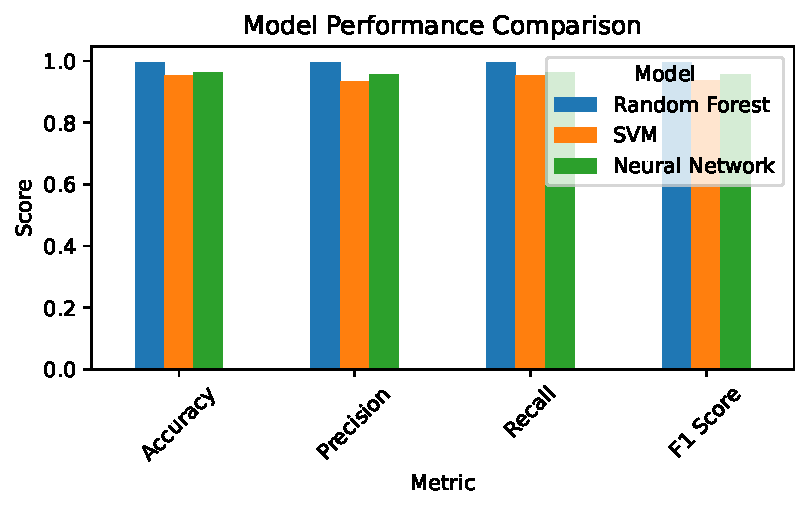
\includegraphics[keepaspectratio]{detecting_bots_on_reddit_code_files/figure-pdf/cell-22-output-4.pdf}}

\pandocbounded{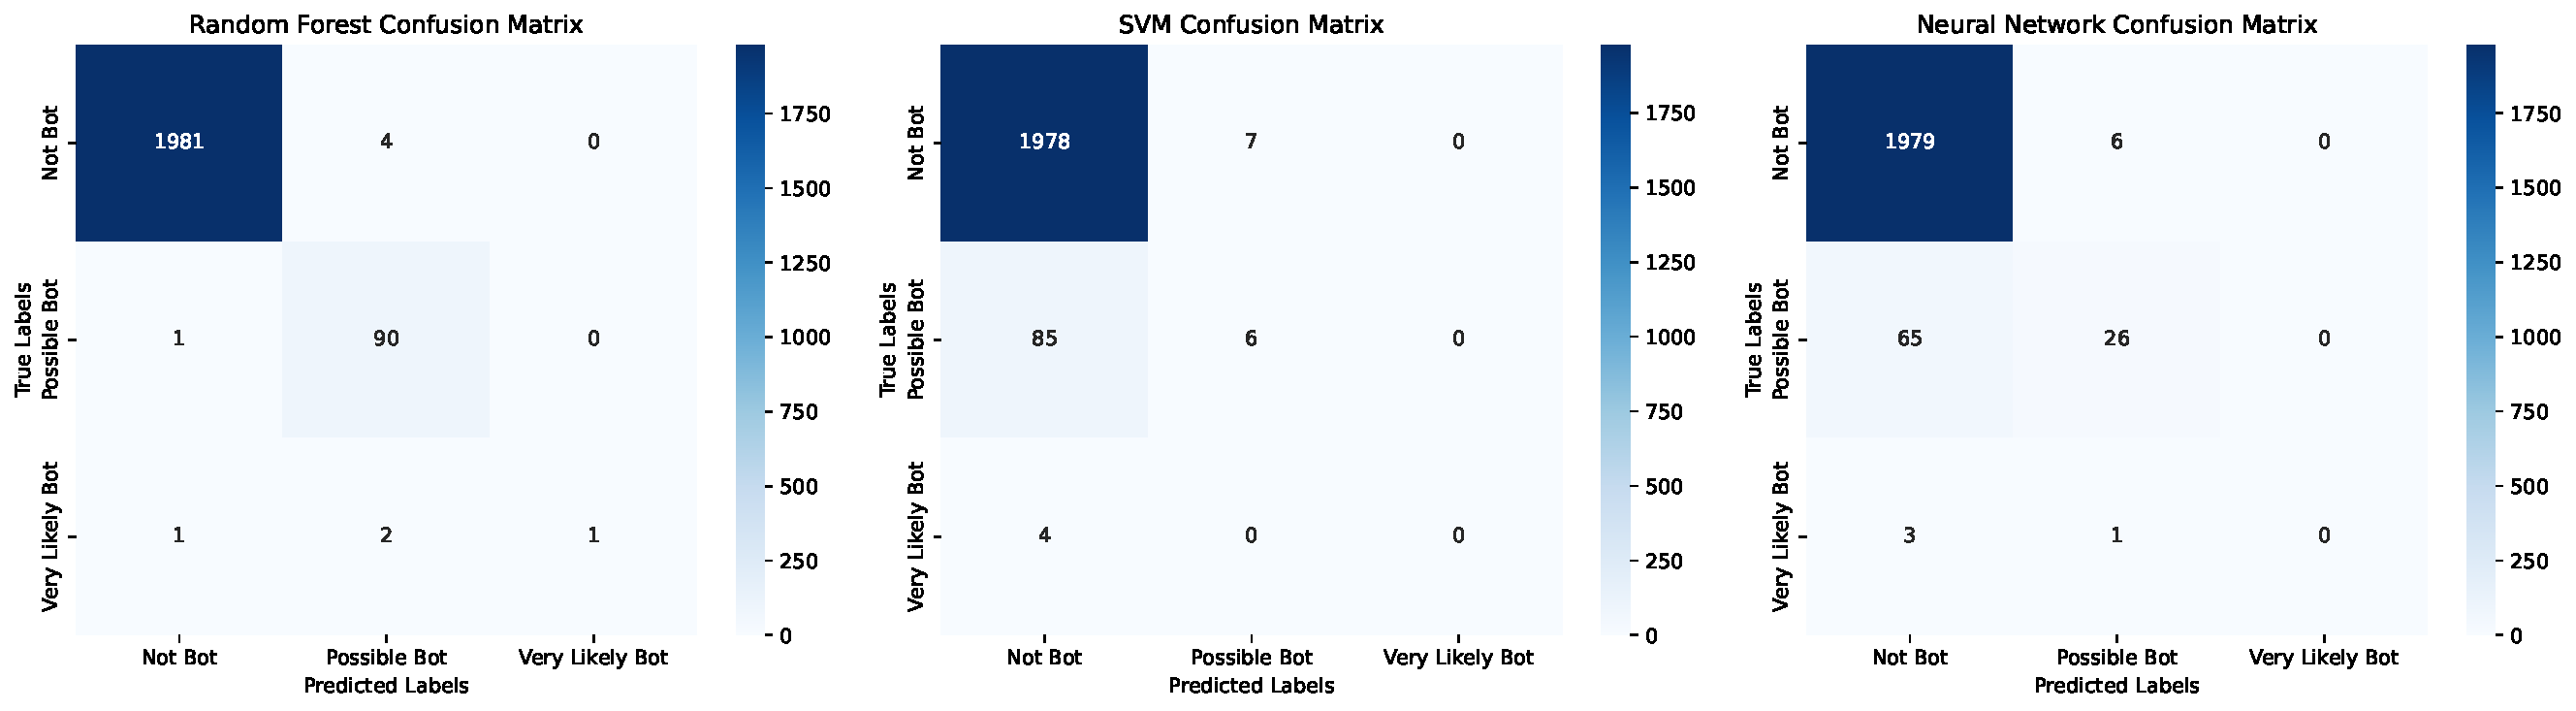
\includegraphics[keepaspectratio]{detecting_bots_on_reddit_code_files/figure-pdf/cell-22-output-5.pdf}}

\pandocbounded{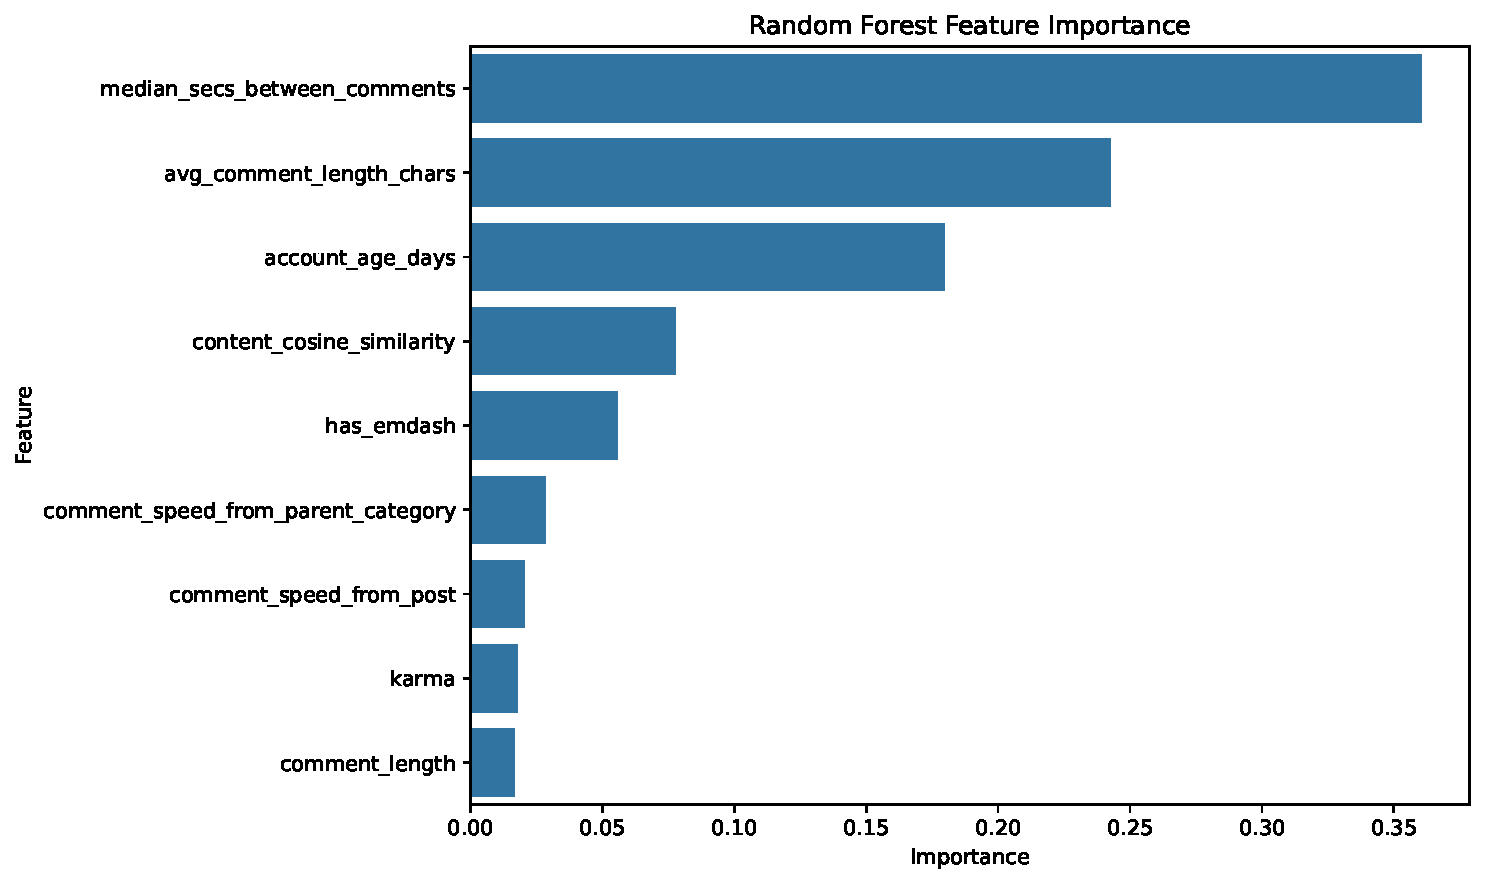
\includegraphics[keepaspectratio]{detecting_bots_on_reddit_code_files/figure-pdf/cell-22-output-6.pdf}}

\begin{Shaded}
\begin{Highlighting}[]
\ImportTok{from}\NormalTok{ sklearn.decomposition }\ImportTok{import}\NormalTok{ PCA}
\ImportTok{from}\NormalTok{ sklearn.cluster }\ImportTok{import}\NormalTok{ KMeans, DBSCAN}
\ImportTok{from}\NormalTok{ sklearn.metrics }\ImportTok{import}\NormalTok{ silhouette\_score}

\CommentTok{\# Prepare features}
\NormalTok{X }\OperatorTok{=}\NormalTok{ user\_level\_data.drop([}\StringTok{\textquotesingle{}comment\_author\textquotesingle{}}\NormalTok{, }\StringTok{\textquotesingle{}bot\_category\textquotesingle{}}\NormalTok{], axis}\OperatorTok{=}\DecValTok{1}\NormalTok{)}

\CommentTok{\# Scale the features}
\NormalTok{scaler }\OperatorTok{=}\NormalTok{ StandardScaler()}
\NormalTok{X\_scaled }\OperatorTok{=}\NormalTok{ scaler.fit\_transform(X)}

\CommentTok{\# Apply PCA for dimensionality reduction}
\NormalTok{pca }\OperatorTok{=}\NormalTok{ PCA(n\_components}\OperatorTok{=}\DecValTok{2}\NormalTok{)  }\CommentTok{\# Reduce to 2 components for easy plotting}
\NormalTok{X\_pca }\OperatorTok{=}\NormalTok{ pca.fit\_transform(X\_scaled)}

\CommentTok{\# Determine optimal number of clusters for K{-}means using Silhouette Score}
\NormalTok{silhouette\_scores }\OperatorTok{=}\NormalTok{ []}
\ControlFlowTok{for}\NormalTok{ n\_clusters }\KeywordTok{in} \BuiltInTok{range}\NormalTok{(}\DecValTok{2}\NormalTok{, }\DecValTok{6}\NormalTok{):  }\CommentTok{\# Try different numbers of clusters}
\NormalTok{    kmeans }\OperatorTok{=}\NormalTok{ KMeans(n\_clusters}\OperatorTok{=}\NormalTok{n\_clusters, random\_state}\OperatorTok{=}\DecValTok{42}\NormalTok{, n\_init}\OperatorTok{=}\DecValTok{10}\NormalTok{)}
\NormalTok{    cluster\_labels }\OperatorTok{=}\NormalTok{ kmeans.fit\_predict(X\_pca)}
\NormalTok{    silhouette\_avg }\OperatorTok{=}\NormalTok{ silhouette\_score(X\_pca, cluster\_labels)}
\NormalTok{    silhouette\_scores.append(silhouette\_avg)}

\CommentTok{\# Select the number of clusters with the highest Silhouette Score}
\NormalTok{optimal\_n\_clusters }\OperatorTok{=} \BuiltInTok{range}\NormalTok{(}\DecValTok{2}\NormalTok{, }\DecValTok{6}\NormalTok{)[silhouette\_scores.index(}\BuiltInTok{max}\NormalTok{(silhouette\_scores))]}

\CommentTok{\# Perform K{-}means clustering with optimal number of clusters}
\NormalTok{kmeans }\OperatorTok{=}\NormalTok{ KMeans(n\_clusters}\OperatorTok{=}\NormalTok{optimal\_n\_clusters, random\_state}\OperatorTok{=}\DecValTok{42}\NormalTok{, n\_init}\OperatorTok{=}\DecValTok{10}\NormalTok{)}
\NormalTok{kmeans\_clusters }\OperatorTok{=}\NormalTok{ kmeans.fit\_predict(X\_pca)}

\CommentTok{\# Determine optimal DBSCAN parameters using Silhouette Score}
\NormalTok{best\_dbscan\_score }\OperatorTok{=} \OperatorTok{{-}}\DecValTok{1}
\NormalTok{optimal\_eps }\OperatorTok{=} \VariableTok{None}
\NormalTok{optimal\_min\_samples }\OperatorTok{=} \VariableTok{None}

\ControlFlowTok{for}\NormalTok{ eps }\KeywordTok{in}\NormalTok{ [}\FloatTok{0.1}\NormalTok{, }\FloatTok{0.5}\NormalTok{, }\FloatTok{1.0}\NormalTok{, }\FloatTok{1.5}\NormalTok{]:}
    \ControlFlowTok{for}\NormalTok{ min\_samples }\KeywordTok{in}\NormalTok{ [}\DecValTok{5}\NormalTok{, }\DecValTok{10}\NormalTok{, }\DecValTok{15}\NormalTok{]:}
\NormalTok{        dbscan }\OperatorTok{=}\NormalTok{ DBSCAN(eps}\OperatorTok{=}\NormalTok{eps, min\_samples}\OperatorTok{=}\NormalTok{min\_samples)}
\NormalTok{        dbscan\_clusters }\OperatorTok{=}\NormalTok{ dbscan.fit\_predict(X\_pca)}
        
        \CommentTok{\# DBSCAN may result in all points being noise (cluster {-}1).  Need at least 2 clusters to calculate silhouette score}
        \ControlFlowTok{if} \BuiltInTok{len}\NormalTok{(}\BuiltInTok{set}\NormalTok{(dbscan\_clusters)) }\OperatorTok{\textgreater{}} \DecValTok{1}\NormalTok{:}
\NormalTok{            dbscan\_score }\OperatorTok{=}\NormalTok{ silhouette\_score(X\_pca, dbscan\_clusters)}
            \ControlFlowTok{if}\NormalTok{ dbscan\_score }\OperatorTok{\textgreater{}}\NormalTok{ best\_dbscan\_score:}
\NormalTok{                best\_dbscan\_score }\OperatorTok{=}\NormalTok{ dbscan\_score}
\NormalTok{                optimal\_eps }\OperatorTok{=}\NormalTok{ eps}
\NormalTok{                optimal\_min\_samples }\OperatorTok{=}\NormalTok{ min\_samples}

\CommentTok{\# Perform DBSCAN clustering with optimal parameters}
\NormalTok{dbscan }\OperatorTok{=}\NormalTok{ DBSCAN(eps}\OperatorTok{=}\NormalTok{optimal\_eps, min\_samples}\OperatorTok{=}\NormalTok{optimal\_min\_samples)  }\CommentTok{\# Adjust eps and min\_samples as needed}
\NormalTok{dbscan\_clusters }\OperatorTok{=}\NormalTok{ dbscan.fit\_predict(X\_pca)}

\CommentTok{\# Create a DataFrame for plotting}
\NormalTok{pca\_df }\OperatorTok{=}\NormalTok{ pd.DataFrame(data}\OperatorTok{=}\NormalTok{X\_pca, columns}\OperatorTok{=}\NormalTok{[}\StringTok{\textquotesingle{}PCA1\textquotesingle{}}\NormalTok{, }\StringTok{\textquotesingle{}PCA2\textquotesingle{}}\NormalTok{])}
\NormalTok{pca\_df[}\StringTok{\textquotesingle{}KMeans Cluster\textquotesingle{}}\NormalTok{] }\OperatorTok{=}\NormalTok{ kmeans\_clusters}
\NormalTok{pca\_df[}\StringTok{\textquotesingle{}DBSCAN Cluster\textquotesingle{}}\NormalTok{] }\OperatorTok{=}\NormalTok{ dbscan\_clusters}
\NormalTok{pca\_df[}\StringTok{\textquotesingle{}Bot Category\textquotesingle{}}\NormalTok{] }\OperatorTok{=}\NormalTok{ y.}\BuiltInTok{map}\NormalTok{(\{}\DecValTok{0}\NormalTok{: }\StringTok{\textquotesingle{}Likely Human\textquotesingle{}}\NormalTok{, }\DecValTok{1}\NormalTok{: }\StringTok{\textquotesingle{}Possible Bot\textquotesingle{}}\NormalTok{, }\DecValTok{2}\NormalTok{: }\StringTok{\textquotesingle{}Likely Bot\textquotesingle{}}\NormalTok{\}).values  }\CommentTok{\# Add actual bot categories for comparison}

\CommentTok{\# Get the loading vectors}
\NormalTok{loadings }\OperatorTok{=}\NormalTok{ pca.components\_}

\CommentTok{\# Determine the most important features for each component}
\NormalTok{feature\_names }\OperatorTok{=}\NormalTok{ X.columns}
\NormalTok{pc1\_loadings }\OperatorTok{=}\NormalTok{ pd.Series(loadings[}\DecValTok{0}\NormalTok{], index}\OperatorTok{=}\NormalTok{feature\_names)}
\NormalTok{pc2\_loadings }\OperatorTok{=}\NormalTok{ pd.Series(loadings[}\DecValTok{1}\NormalTok{], index}\OperatorTok{=}\NormalTok{feature\_names)}

\CommentTok{\# Identify top features for each component}
\NormalTok{pc1\_top\_features }\OperatorTok{=}\NormalTok{ pc1\_loadings.}\BuiltInTok{abs}\NormalTok{().nlargest(}\DecValTok{3}\NormalTok{).index.tolist()}
\NormalTok{pc2\_top\_features }\OperatorTok{=}\NormalTok{ pc2\_loadings.}\BuiltInTok{abs}\NormalTok{().nlargest(}\DecValTok{3}\NormalTok{).index.tolist()}

\CommentTok{\# Label the principal components}
\NormalTok{pc1\_label }\OperatorTok{=} \SpecialStringTok{f"PC1 (}\SpecialCharTok{\{}\StringTok{\textquotesingle{}, \textquotesingle{}}\SpecialCharTok{.}\NormalTok{join(pc1\_top\_features)}\SpecialCharTok{\}}\SpecialStringTok{)"}
\NormalTok{pc2\_label }\OperatorTok{=} \SpecialStringTok{f"PC2 (}\SpecialCharTok{\{}\StringTok{\textquotesingle{}, \textquotesingle{}}\SpecialCharTok{.}\NormalTok{join(pc2\_top\_features)}\SpecialCharTok{\}}\SpecialStringTok{)"}
\end{Highlighting}
\end{Shaded}

\begin{Shaded}
\begin{Highlighting}[]
\CommentTok{\# Visualize the KMeans clusters}
\NormalTok{plt.figure(figsize}\OperatorTok{=}\NormalTok{(}\DecValTok{12}\NormalTok{, }\DecValTok{10}\NormalTok{))}
\NormalTok{plt.subplot(}\DecValTok{2}\NormalTok{, }\DecValTok{1}\NormalTok{, }\DecValTok{1}\NormalTok{)}
\NormalTok{sns.scatterplot(x}\OperatorTok{=}\StringTok{\textquotesingle{}PCA1\textquotesingle{}}\NormalTok{, y}\OperatorTok{=}\StringTok{\textquotesingle{}PCA2\textquotesingle{}}\NormalTok{, hue}\OperatorTok{=}\StringTok{\textquotesingle{}KMeans Cluster\textquotesingle{}}\NormalTok{, style}\OperatorTok{=}\StringTok{\textquotesingle{}Bot Category\textquotesingle{}}\NormalTok{, data}\OperatorTok{=}\NormalTok{pca\_df, palette}\OperatorTok{=}\StringTok{\textquotesingle{}viridis\textquotesingle{}}\NormalTok{, alpha}\OperatorTok{=}\FloatTok{0.7}\NormalTok{, s}\OperatorTok{=}\DecValTok{100}\NormalTok{)}
\NormalTok{plt.title(}\StringTok{\textquotesingle{}K{-}Means Clustering of User Features\textquotesingle{}}\NormalTok{)}
\NormalTok{plt.xlabel(pc1\_label)}
\NormalTok{plt.ylabel(pc2\_label)}

\CommentTok{\# Visualize the DBSCAN clusters}
\NormalTok{plt.subplot(}\DecValTok{2}\NormalTok{, }\DecValTok{1}\NormalTok{, }\DecValTok{2}\NormalTok{)}
\NormalTok{sns.scatterplot(x}\OperatorTok{=}\StringTok{\textquotesingle{}PCA1\textquotesingle{}}\NormalTok{, y}\OperatorTok{=}\StringTok{\textquotesingle{}PCA2\textquotesingle{}}\NormalTok{, hue}\OperatorTok{=}\StringTok{\textquotesingle{}DBSCAN Cluster\textquotesingle{}}\NormalTok{, style}\OperatorTok{=}\StringTok{\textquotesingle{}Bot Category\textquotesingle{}}\NormalTok{, data}\OperatorTok{=}\NormalTok{pca\_df, palette}\OperatorTok{=}\StringTok{\textquotesingle{}viridis\textquotesingle{}}\NormalTok{, alpha}\OperatorTok{=}\FloatTok{0.7}\NormalTok{, s}\OperatorTok{=}\DecValTok{100}\NormalTok{)}
\NormalTok{plt.title(}\StringTok{\textquotesingle{}DBSCAN Clustering of User Features\textquotesingle{}}\NormalTok{)}
\NormalTok{plt.xlabel(pc1\_label)}
\NormalTok{plt.ylabel(pc2\_label)}

\NormalTok{plt.tight\_layout()}
\NormalTok{plt.show()}
\end{Highlighting}
\end{Shaded}

\pandocbounded{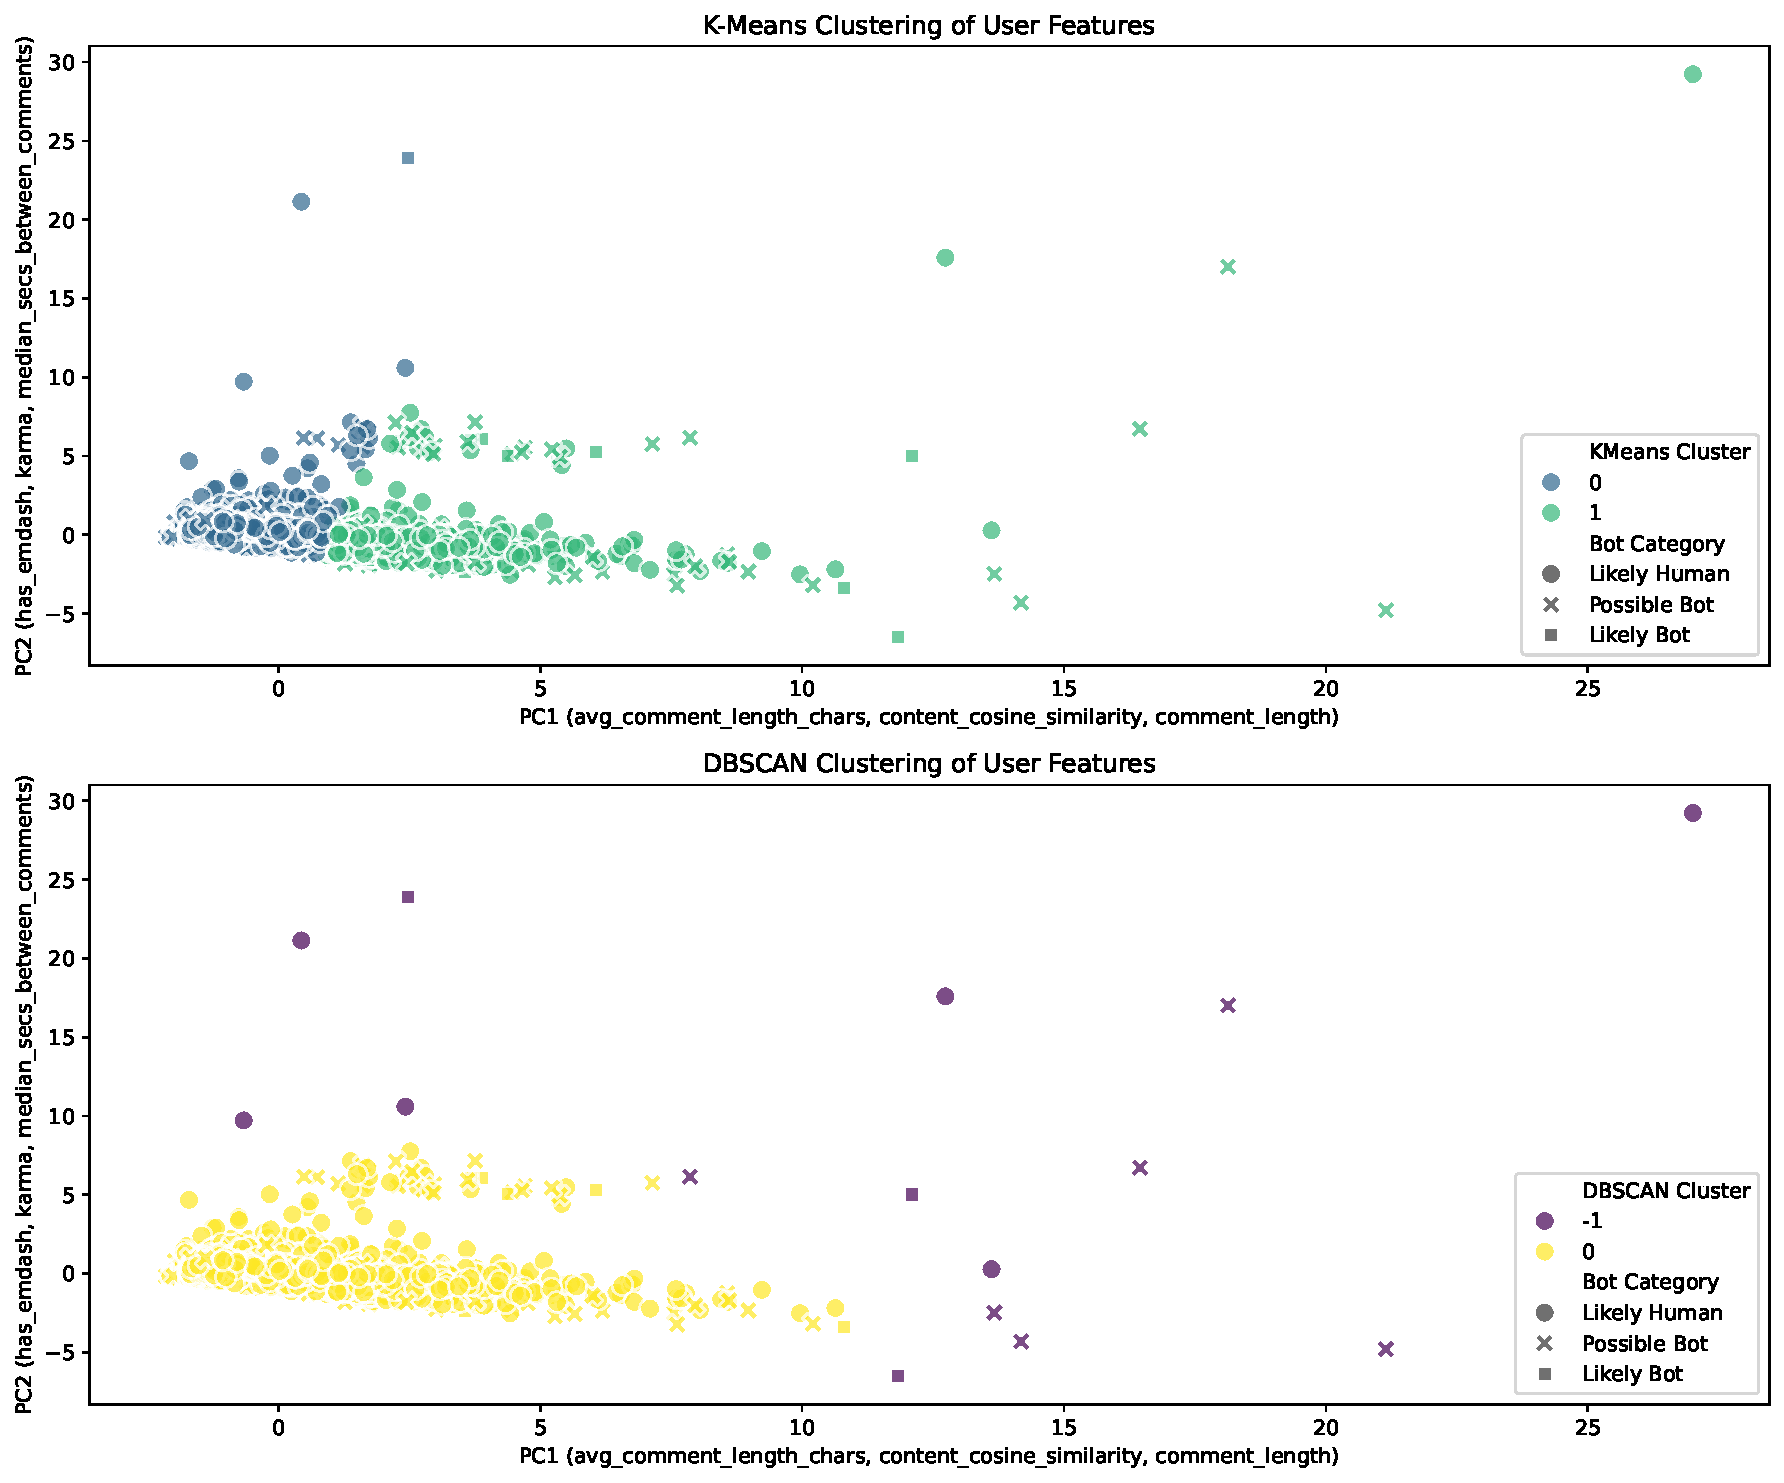
\includegraphics[keepaspectratio]{detecting_bots_on_reddit_code_files/figure-pdf/cell-24-output-1.pdf}}

\begin{Shaded}
\begin{Highlighting}[]
\ImportTok{import}\NormalTok{ pandas }\ImportTok{as}\NormalTok{ pd}
\ImportTok{import}\NormalTok{ numpy }\ImportTok{as}\NormalTok{ np}
\ImportTok{import}\NormalTok{ seaborn }\ImportTok{as}\NormalTok{ sns}
\ImportTok{from}\NormalTok{ nltk.sentiment }\ImportTok{import}\NormalTok{ SentimentIntensityAnalyzer}
\ImportTok{from}\NormalTok{ textblob }\ImportTok{import}\NormalTok{ TextBlob}
\ImportTok{import}\NormalTok{ re}
\ImportTok{from}\NormalTok{ collections }\ImportTok{import}\NormalTok{ Counter}
\ImportTok{from}\NormalTok{ wordcloud }\ImportTok{import}\NormalTok{ WordCloud}
\ImportTok{import}\NormalTok{ nltk}
\ImportTok{from}\NormalTok{ nltk.tokenize }\ImportTok{import}\NormalTok{ word\_tokenize}
\ImportTok{from}\NormalTok{ nltk.corpus }\ImportTok{import}\NormalTok{ stopwords}
\ImportTok{import}\NormalTok{ string}
\ImportTok{from}\NormalTok{ sklearn.feature\_extraction.text }\ImportTok{import}\NormalTok{ CountVectorizer, TfidfVectorizer}
\ImportTok{import}\NormalTok{ textstat}
\ImportTok{from}\NormalTok{ nrclex }\ImportTok{import}\NormalTok{ NRCLex}

\CommentTok{\# Import necessary libraries}
\ImportTok{import}\NormalTok{ matplotlib.pyplot }\ImportTok{as}\NormalTok{ plt}

\CommentTok{\# Download necessary NLTK resources}
\NormalTok{nltk.download(}\StringTok{\textquotesingle{}punkt\textquotesingle{}}\NormalTok{, quiet}\OperatorTok{=}\VariableTok{True}\NormalTok{)}
\NormalTok{nltk.download(}\StringTok{\textquotesingle{}stopwords\textquotesingle{}}\NormalTok{, quiet}\OperatorTok{=}\VariableTok{True}\NormalTok{)}
\NormalTok{nltk.download(}\StringTok{\textquotesingle{}vader\_lexicon\textquotesingle{}}\NormalTok{, quiet}\OperatorTok{=}\VariableTok{True}\NormalTok{)}

\CommentTok{\# Create a filter removing AutoModerator and separating humans from bots}
\NormalTok{ml\_features\_filtered }\OperatorTok{=}\NormalTok{ ml\_features[ml\_features[}\StringTok{\textquotesingle{}comment\_author\textquotesingle{}}\NormalTok{] }\OperatorTok{!=} \StringTok{\textquotesingle{}AutoModerator\textquotesingle{}}\NormalTok{].copy()}

\CommentTok{\# Add a \textquotesingle{}user\_type\textquotesingle{} column}
\NormalTok{ml\_features\_filtered[}\StringTok{\textquotesingle{}user\_type\textquotesingle{}}\NormalTok{] }\OperatorTok{=} \StringTok{\textquotesingle{}Human\textquotesingle{}}
\NormalTok{ml\_features\_filtered.loc[ml\_features\_filtered[}\StringTok{\textquotesingle{}possible\_bot\textquotesingle{}}\NormalTok{] }\OperatorTok{==} \DecValTok{1}\NormalTok{, }\StringTok{\textquotesingle{}user\_type\textquotesingle{}}\NormalTok{] }\OperatorTok{=} \StringTok{\textquotesingle{}Bot\textquotesingle{}}
\NormalTok{ml\_features\_filtered.loc[ml\_features\_filtered[}\StringTok{\textquotesingle{}very\_likely\_bot\textquotesingle{}}\NormalTok{] }\OperatorTok{==} \DecValTok{1}\NormalTok{, }\StringTok{\textquotesingle{}user\_type\textquotesingle{}}\NormalTok{] }\OperatorTok{=} \StringTok{\textquotesingle{}Bot\textquotesingle{}}

\CommentTok{\# VADER Sentiment Analysis}
\NormalTok{analyzer }\OperatorTok{=}\NormalTok{ SentimentIntensityAnalyzer()}

\CommentTok{\# Add sentiment scores}
\NormalTok{ml\_features\_filtered[}\StringTok{\textquotesingle{}vader\_compound\textquotesingle{}}\NormalTok{] }\OperatorTok{=}\NormalTok{ ml\_features\_filtered[}\StringTok{\textquotesingle{}comment\_body\textquotesingle{}}\NormalTok{].}\BuiltInTok{apply}\NormalTok{(}\KeywordTok{lambda}\NormalTok{ x: analyzer.polarity\_scores(x)[}\StringTok{\textquotesingle{}compound\textquotesingle{}}\NormalTok{])}
\NormalTok{ml\_features\_filtered[}\StringTok{\textquotesingle{}vader\_pos\textquotesingle{}}\NormalTok{] }\OperatorTok{=}\NormalTok{ ml\_features\_filtered[}\StringTok{\textquotesingle{}comment\_body\textquotesingle{}}\NormalTok{].}\BuiltInTok{apply}\NormalTok{(}\KeywordTok{lambda}\NormalTok{ x: analyzer.polarity\_scores(x)[}\StringTok{\textquotesingle{}pos\textquotesingle{}}\NormalTok{])}
\NormalTok{ml\_features\_filtered[}\StringTok{\textquotesingle{}vader\_neg\textquotesingle{}}\NormalTok{] }\OperatorTok{=}\NormalTok{ ml\_features\_filtered[}\StringTok{\textquotesingle{}comment\_body\textquotesingle{}}\NormalTok{].}\BuiltInTok{apply}\NormalTok{(}\KeywordTok{lambda}\NormalTok{ x: analyzer.polarity\_scores(x)[}\StringTok{\textquotesingle{}neg\textquotesingle{}}\NormalTok{])}
\NormalTok{ml\_features\_filtered[}\StringTok{\textquotesingle{}vader\_neu\textquotesingle{}}\NormalTok{] }\OperatorTok{=}\NormalTok{ ml\_features\_filtered[}\StringTok{\textquotesingle{}comment\_body\textquotesingle{}}\NormalTok{].}\BuiltInTok{apply}\NormalTok{(}\KeywordTok{lambda}\NormalTok{ x: analyzer.polarity\_scores(x)[}\StringTok{\textquotesingle{}neu\textquotesingle{}}\NormalTok{])}

\CommentTok{\# Calculate text complexity metrics}
\NormalTok{ml\_features\_filtered[}\StringTok{\textquotesingle{}readability\_score\textquotesingle{}}\NormalTok{] }\OperatorTok{=}\NormalTok{ ml\_features\_filtered[}\StringTok{\textquotesingle{}comment\_body\textquotesingle{}}\NormalTok{].}\BuiltInTok{apply}\NormalTok{(}\KeywordTok{lambda}\NormalTok{ x: textstat.flesch\_reading\_ease(x))}
\NormalTok{ml\_features\_filtered[}\StringTok{\textquotesingle{}complexity\_score\textquotesingle{}}\NormalTok{] }\OperatorTok{=}\NormalTok{ ml\_features\_filtered[}\StringTok{\textquotesingle{}comment\_body\textquotesingle{}}\NormalTok{].}\BuiltInTok{apply}\NormalTok{(}\KeywordTok{lambda}\NormalTok{ x: textstat.gunning\_fog(x))}

\CommentTok{\# Function to detect slang or informal language}
\KeywordTok{def}\NormalTok{ contains\_slang(text):}
    \CommentTok{\# Simple slang detection based on common patterns}
\NormalTok{    slang\_patterns }\OperatorTok{=}\NormalTok{ [}\VerbatimStringTok{r\textquotesingle{}\textbackslash{}blol\textbackslash{}b\textquotesingle{}}\NormalTok{, }\VerbatimStringTok{r\textquotesingle{}\textbackslash{}bomg\textbackslash{}b\textquotesingle{}}\NormalTok{, }\VerbatimStringTok{r\textquotesingle{}\textbackslash{}bbtw\textbackslash{}b\textquotesingle{}}\NormalTok{, }\VerbatimStringTok{r\textquotesingle{}\textbackslash{}bidk\textbackslash{}b\textquotesingle{}}\NormalTok{, }\VerbatimStringTok{r\textquotesingle{}\textbackslash{}bimo\textbackslash{}b\textquotesingle{}}\NormalTok{, }\VerbatimStringTok{r\textquotesingle{}\textbackslash{}bfyi\textbackslash{}b\textquotesingle{}}\NormalTok{, }
                      \VerbatimStringTok{r\textquotesingle{}\textbackslash{}bsmh\textbackslash{}b\textquotesingle{}}\NormalTok{, }\VerbatimStringTok{r\textquotesingle{}\textbackslash{}bwtf\textbackslash{}b\textquotesingle{}}\NormalTok{, }\VerbatimStringTok{r\textquotesingle{}\textbackslash{}baf\textbackslash{}b\textquotesingle{}}\NormalTok{, }\VerbatimStringTok{r\textquotesingle{}\textbackslash{}bfr\textbackslash{}b\textquotesingle{}}\NormalTok{, }\VerbatimStringTok{r\textquotesingle{}\textbackslash{}byolo\textbackslash{}b\textquotesingle{}}\NormalTok{, }\VerbatimStringTok{r\textquotesingle{}\textbackslash{}btbh\textbackslash{}b\textquotesingle{}}\NormalTok{,}
                      \VerbatimStringTok{r\textquotesingle{}\textbackslash{}brofl\textbackslash{}b\textquotesingle{}}\NormalTok{, }\VerbatimStringTok{r\textquotesingle{}\textbackslash{}blmao\textbackslash{}b\textquotesingle{}}\NormalTok{, }\VerbatimStringTok{r\textquotesingle{}\textbackslash{}blmfao\textbackslash{}b\textquotesingle{}}\NormalTok{, }\VerbatimStringTok{r\textquotesingle{}\textbackslash{}bbrb\textbackslash{}b\textquotesingle{}}\NormalTok{, }\VerbatimStringTok{r\textquotesingle{}\textbackslash{}bafaik\textbackslash{}b\textquotesingle{}}\NormalTok{,}
                      \VerbatimStringTok{r\textquotesingle{}\textbackslash{}bftw\textbackslash{}b\textquotesingle{}}\NormalTok{, }\VerbatimStringTok{r\textquotesingle{}\textbackslash{}bfml\textbackslash{}b\textquotesingle{}}\NormalTok{, }\VerbatimStringTok{r\textquotesingle{}\textbackslash{}bomfg\textbackslash{}b\textquotesingle{}}\NormalTok{, }\VerbatimStringTok{r\textquotesingle{}\textbackslash{}bidc\textbackslash{}b\textquotesingle{}}\NormalTok{, }\VerbatimStringTok{r\textquotesingle{}\textbackslash{}bimho\textbackslash{}b\textquotesingle{}}\NormalTok{]}
    
    \ControlFlowTok{for}\NormalTok{ pattern }\KeywordTok{in}\NormalTok{ slang\_patterns:}
        \ControlFlowTok{if}\NormalTok{ re.search(pattern, text.lower()):}
            \ControlFlowTok{return} \DecValTok{1}
    \ControlFlowTok{return} \DecValTok{0}

\CommentTok{\# Function to count exclamation and question marks}
\KeywordTok{def}\NormalTok{ count\_punctuation(text):}
\NormalTok{    exclamation\_count }\OperatorTok{=}\NormalTok{ text.count(}\StringTok{\textquotesingle{}!\textquotesingle{}}\NormalTok{)}
\NormalTok{    question\_count }\OperatorTok{=}\NormalTok{ text.count(}\StringTok{\textquotesingle{}?\textquotesingle{}}\NormalTok{)}
    \ControlFlowTok{return}\NormalTok{ exclamation\_count, question\_count}

\CommentTok{\# Apply the slang detection and punctuation counting}
\NormalTok{ml\_features\_filtered[}\StringTok{\textquotesingle{}contains\_slang\textquotesingle{}}\NormalTok{] }\OperatorTok{=}\NormalTok{ ml\_features\_filtered[}\StringTok{\textquotesingle{}comment\_body\textquotesingle{}}\NormalTok{].}\BuiltInTok{apply}\NormalTok{(contains\_slang)}
\NormalTok{ml\_features\_filtered[}\StringTok{\textquotesingle{}exclamation\_count\textquotesingle{}}\NormalTok{] }\OperatorTok{=}\NormalTok{ ml\_features\_filtered[}\StringTok{\textquotesingle{}comment\_body\textquotesingle{}}\NormalTok{].}\BuiltInTok{apply}\NormalTok{(}\KeywordTok{lambda}\NormalTok{ x: count\_punctuation(x)[}\DecValTok{0}\NormalTok{])}
\NormalTok{ml\_features\_filtered[}\StringTok{\textquotesingle{}question\_count\textquotesingle{}}\NormalTok{] }\OperatorTok{=}\NormalTok{ ml\_features\_filtered[}\StringTok{\textquotesingle{}comment\_body\textquotesingle{}}\NormalTok{].}\BuiltInTok{apply}\NormalTok{(}\KeywordTok{lambda}\NormalTok{ x: count\_punctuation(x)[}\DecValTok{1}\NormalTok{])}

\CommentTok{\# Emotion Detection using NRCLex}
\KeywordTok{def}\NormalTok{ extract\_emotions(text):}
\NormalTok{    emotion\_scores }\OperatorTok{=}\NormalTok{ NRCLex(text).affect\_frequencies}
    \ControlFlowTok{return}\NormalTok{ emotion\_scores}

\CommentTok{\# Extract a sample due to computational constraints}
\NormalTok{sample\_size }\OperatorTok{=} \BuiltInTok{min}\NormalTok{(}\DecValTok{1000}\NormalTok{, }\BuiltInTok{len}\NormalTok{(ml\_features\_filtered))}
\NormalTok{emotions\_sample }\OperatorTok{=}\NormalTok{ ml\_features\_filtered.sample(sample\_size, random\_state}\OperatorTok{=}\DecValTok{42}\NormalTok{)}

\CommentTok{\# Apply emotion extraction}
\NormalTok{emotions\_df }\OperatorTok{=}\NormalTok{ pd.DataFrame([extract\_emotions(text) }\ControlFlowTok{for}\NormalTok{ text }\KeywordTok{in}\NormalTok{ emotions\_sample[}\StringTok{\textquotesingle{}comment\_body\textquotesingle{}}\NormalTok{]])}
\NormalTok{emotions\_sample }\OperatorTok{=}\NormalTok{ pd.concat([emotions\_sample.reset\_index(drop}\OperatorTok{=}\VariableTok{True}\NormalTok{), emotions\_df.reset\_index(drop}\OperatorTok{=}\VariableTok{True}\NormalTok{)], axis}\OperatorTok{=}\DecValTok{1}\NormalTok{)}

\CommentTok{\# Create visualization for sentiment comparison}
\NormalTok{plt.figure(figsize}\OperatorTok{=}\NormalTok{(}\DecValTok{16}\NormalTok{, }\DecValTok{12}\NormalTok{))}

\CommentTok{\# 1. VADER Sentiment Distribution}
\NormalTok{plt.subplot(}\DecValTok{2}\NormalTok{, }\DecValTok{2}\NormalTok{, }\DecValTok{1}\NormalTok{)}
\NormalTok{sns.boxplot(x}\OperatorTok{=}\StringTok{\textquotesingle{}user\_type\textquotesingle{}}\NormalTok{, y}\OperatorTok{=}\StringTok{\textquotesingle{}vader\_compound\textquotesingle{}}\NormalTok{, data}\OperatorTok{=}\NormalTok{ml\_features\_filtered)}
\NormalTok{plt.title(}\StringTok{\textquotesingle{}VADER Sentiment Scores by User Type\textquotesingle{}}\NormalTok{)}
\NormalTok{plt.xlabel(}\StringTok{\textquotesingle{}User Type\textquotesingle{}}\NormalTok{)}
\NormalTok{plt.ylabel(}\StringTok{\textquotesingle{}Compound Sentiment Score\textquotesingle{}}\NormalTok{)}

\CommentTok{\# 2. Emotion Comparison}
\NormalTok{plt.subplot(}\DecValTok{2}\NormalTok{, }\DecValTok{2}\NormalTok{, }\DecValTok{2}\NormalTok{)}
\NormalTok{emotion\_cols }\OperatorTok{=}\NormalTok{ [}\StringTok{\textquotesingle{}fear\textquotesingle{}}\NormalTok{, }\StringTok{\textquotesingle{}anger\textquotesingle{}}\NormalTok{, }\StringTok{\textquotesingle{}anticipation\textquotesingle{}}\NormalTok{, }\StringTok{\textquotesingle{}trust\textquotesingle{}}\NormalTok{, }\StringTok{\textquotesingle{}surprise\textquotesingle{}}\NormalTok{, }\StringTok{\textquotesingle{}sadness\textquotesingle{}}\NormalTok{, }\StringTok{\textquotesingle{}disgust\textquotesingle{}}\NormalTok{, }\StringTok{\textquotesingle{}joy\textquotesingle{}}\NormalTok{]}
\NormalTok{emotions\_by\_type }\OperatorTok{=}\NormalTok{ emotions\_sample.groupby(}\StringTok{\textquotesingle{}user\_type\textquotesingle{}}\NormalTok{)[emotion\_cols].mean()}
\NormalTok{emotions\_by\_type.T.plot(kind}\OperatorTok{=}\StringTok{\textquotesingle{}bar\textquotesingle{}}\NormalTok{, ax}\OperatorTok{=}\NormalTok{plt.gca())}
\NormalTok{plt.title(}\StringTok{\textquotesingle{}Average Emotion Intensity by User Type\textquotesingle{}}\NormalTok{)}
\NormalTok{plt.xlabel(}\StringTok{\textquotesingle{}Emotion\textquotesingle{}}\NormalTok{)}
\NormalTok{plt.ylabel(}\StringTok{\textquotesingle{}Average Intensity\textquotesingle{}}\NormalTok{)}
\NormalTok{plt.xticks(rotation}\OperatorTok{=}\DecValTok{45}\NormalTok{)}
\NormalTok{plt.legend(title}\OperatorTok{=}\StringTok{\textquotesingle{}User Type\textquotesingle{}}\NormalTok{)}

\CommentTok{\# 3. Text Complexity}
\NormalTok{plt.subplot(}\DecValTok{2}\NormalTok{, }\DecValTok{2}\NormalTok{, }\DecValTok{3}\NormalTok{)}
\NormalTok{sns.boxplot(x}\OperatorTok{=}\StringTok{\textquotesingle{}user\_type\textquotesingle{}}\NormalTok{, y}\OperatorTok{=}\StringTok{\textquotesingle{}readability\_score\textquotesingle{}}\NormalTok{, data}\OperatorTok{=}\NormalTok{ml\_features\_filtered)}
\NormalTok{plt.title(}\StringTok{\textquotesingle{}Text Readability by User Type\textquotesingle{}}\NormalTok{)}
\NormalTok{plt.xlabel(}\StringTok{\textquotesingle{}User Type\textquotesingle{}}\NormalTok{)}
\NormalTok{plt.ylabel(}\StringTok{\textquotesingle{}Flesch Reading Ease Score\textquotesingle{}}\NormalTok{)}

\CommentTok{\# 4. Slang Usage}
\NormalTok{plt.subplot(}\DecValTok{2}\NormalTok{, }\DecValTok{2}\NormalTok{, }\DecValTok{4}\NormalTok{)}
\NormalTok{slang\_by\_type }\OperatorTok{=}\NormalTok{ ml\_features\_filtered.groupby(}\StringTok{\textquotesingle{}user\_type\textquotesingle{}}\NormalTok{)[}\StringTok{\textquotesingle{}contains\_slang\textquotesingle{}}\NormalTok{].mean()}
\NormalTok{slang\_by\_type.plot(kind}\OperatorTok{=}\StringTok{\textquotesingle{}bar\textquotesingle{}}\NormalTok{, ax}\OperatorTok{=}\NormalTok{plt.gca())}
\NormalTok{plt.title(}\StringTok{\textquotesingle{}Slang Usage by User Type\textquotesingle{}}\NormalTok{)}
\NormalTok{plt.xlabel(}\StringTok{\textquotesingle{}User Type\textquotesingle{}}\NormalTok{)}
\NormalTok{plt.ylabel(}\StringTok{\textquotesingle{}Proportion of Comments with Slang\textquotesingle{}}\NormalTok{)}

\NormalTok{plt.tight\_layout()}
\NormalTok{plt.show()}

\CommentTok{\# Extract common words by user type}
\KeywordTok{def}\NormalTok{ get\_common\_words(texts, n}\OperatorTok{=}\DecValTok{20}\NormalTok{):}
    \CommentTok{\# Tokenize and clean}
\NormalTok{    stop\_words }\OperatorTok{=} \BuiltInTok{set}\NormalTok{(stopwords.words(}\StringTok{\textquotesingle{}english\textquotesingle{}}\NormalTok{))}
\NormalTok{    stop\_words.update([}\StringTok{\textquotesingle{}would\textquotesingle{}}\NormalTok{, }\StringTok{\textquotesingle{}could\textquotesingle{}}\NormalTok{, }\StringTok{\textquotesingle{}also\textquotesingle{}}\NormalTok{, }\StringTok{\textquotesingle{}one\textquotesingle{}}\NormalTok{, }\StringTok{\textquotesingle{}like\textquotesingle{}}\NormalTok{, }\StringTok{\textquotesingle{}get\textquotesingle{}}\NormalTok{, }\StringTok{\textquotesingle{}even\textquotesingle{}}\NormalTok{, }\StringTok{\textquotesingle{}say\textquotesingle{}}\NormalTok{, }\StringTok{\textquotesingle{}said\textquotesingle{}}\NormalTok{, }\StringTok{\textquotesingle{}make\textquotesingle{}}\NormalTok{, }\StringTok{\textquotesingle{}think\textquotesingle{}}\NormalTok{, }\StringTok{\textquotesingle{}know\textquotesingle{}}\NormalTok{])}
    
\NormalTok{    words }\OperatorTok{=}\NormalTok{ []}
    \ControlFlowTok{for}\NormalTok{ text }\KeywordTok{in}\NormalTok{ texts:}
\NormalTok{        tokens }\OperatorTok{=}\NormalTok{ word\_tokenize(text.lower())}
        \CommentTok{\# Remove stopwords, punctuation, and non{-}alphabetic tokens}
\NormalTok{        words.extend([word }\ControlFlowTok{for}\NormalTok{ word }\KeywordTok{in}\NormalTok{ tokens }\ControlFlowTok{if}\NormalTok{ word }\KeywordTok{not} \KeywordTok{in}\NormalTok{ stop\_words }
                     \KeywordTok{and}\NormalTok{ word }\KeywordTok{not} \KeywordTok{in}\NormalTok{ string.punctuation }
                     \KeywordTok{and}\NormalTok{ word.isalpha() }
                     \KeywordTok{and} \BuiltInTok{len}\NormalTok{(word) }\OperatorTok{\textgreater{}} \DecValTok{2}\NormalTok{]) }\CommentTok{\#this line filters out words of length 3 or more}
    
    \ControlFlowTok{return}\NormalTok{ Counter(words).most\_common(n)}

\CommentTok{\# Get most common words for humans and bots}
\NormalTok{human\_texts }\OperatorTok{=}\NormalTok{ ml\_features\_filtered[ml\_features\_filtered[}\StringTok{\textquotesingle{}user\_type\textquotesingle{}}\NormalTok{] }\OperatorTok{==} \StringTok{\textquotesingle{}Human\textquotesingle{}}\NormalTok{][}\StringTok{\textquotesingle{}comment\_body\textquotesingle{}}\NormalTok{].tolist()}
\NormalTok{bot\_texts }\OperatorTok{=}\NormalTok{ ml\_features\_filtered[ml\_features\_filtered[}\StringTok{\textquotesingle{}user\_type\textquotesingle{}}\NormalTok{] }\OperatorTok{==} \StringTok{\textquotesingle{}Bot\textquotesingle{}}\NormalTok{][}\StringTok{\textquotesingle{}comment\_body\textquotesingle{}}\NormalTok{].tolist()}

\NormalTok{human\_common\_words }\OperatorTok{=}\NormalTok{ get\_common\_words(human\_texts)}
\NormalTok{bot\_common\_words }\OperatorTok{=}\NormalTok{ get\_common\_words(bot\_texts)}

\CommentTok{\# Create word clouds}
\NormalTok{plt.figure(figsize}\OperatorTok{=}\NormalTok{(}\DecValTok{16}\NormalTok{, }\DecValTok{8}\NormalTok{))}

\CommentTok{\# Word cloud for humans}
\NormalTok{plt.subplot(}\DecValTok{1}\NormalTok{, }\DecValTok{2}\NormalTok{, }\DecValTok{1}\NormalTok{)}
\NormalTok{human\_wordcloud }\OperatorTok{=}\NormalTok{ WordCloud(width}\OperatorTok{=}\DecValTok{800}\NormalTok{, height}\OperatorTok{=}\DecValTok{400}\NormalTok{, background\_color}\OperatorTok{=}\StringTok{\textquotesingle{}white\textquotesingle{}}\NormalTok{, }
\NormalTok{                           max\_words}\OperatorTok{=}\DecValTok{100}\NormalTok{, colormap}\OperatorTok{=}\StringTok{\textquotesingle{}viridis\textquotesingle{}}\NormalTok{, min\_word\_length}\OperatorTok{=}\DecValTok{3}\NormalTok{).generate(}\StringTok{\textquotesingle{} \textquotesingle{}}\NormalTok{.join(human\_texts))}
\NormalTok{plt.imshow(human\_wordcloud, interpolation}\OperatorTok{=}\StringTok{\textquotesingle{}bilinear\textquotesingle{}}\NormalTok{)}
\NormalTok{plt.title(}\StringTok{\textquotesingle{}Word Cloud for Human Comments\textquotesingle{}}\NormalTok{)}
\NormalTok{plt.axis(}\StringTok{\textquotesingle{}off\textquotesingle{}}\NormalTok{)}

\CommentTok{\# Word cloud for bots}
\NormalTok{plt.subplot(}\DecValTok{1}\NormalTok{, }\DecValTok{2}\NormalTok{, }\DecValTok{2}\NormalTok{)}
\NormalTok{bot\_wordcloud }\OperatorTok{=}\NormalTok{ WordCloud(width}\OperatorTok{=}\DecValTok{800}\NormalTok{, height}\OperatorTok{=}\DecValTok{400}\NormalTok{, background\_color}\OperatorTok{=}\StringTok{\textquotesingle{}white\textquotesingle{}}\NormalTok{, }
\NormalTok{                         max\_words}\OperatorTok{=}\DecValTok{100}\NormalTok{, colormap}\OperatorTok{=}\StringTok{\textquotesingle{}plasma\textquotesingle{}}\NormalTok{, min\_word\_length}\OperatorTok{=}\DecValTok{3}\NormalTok{).generate(}\StringTok{\textquotesingle{} \textquotesingle{}}\NormalTok{.join(bot\_texts))}
\NormalTok{plt.imshow(bot\_wordcloud, interpolation}\OperatorTok{=}\StringTok{\textquotesingle{}bilinear\textquotesingle{}}\NormalTok{)}
\NormalTok{plt.title(}\StringTok{\textquotesingle{}Word Cloud for Bot Comments\textquotesingle{}}\NormalTok{)}
\NormalTok{plt.axis(}\StringTok{\textquotesingle{}off\textquotesingle{}}\NormalTok{)}

\NormalTok{plt.tight\_layout()}
\NormalTok{plt.show()}

\CommentTok{\# Compare linguistic style metrics}
\NormalTok{plt.figure(figsize}\OperatorTok{=}\NormalTok{(}\DecValTok{16}\NormalTok{, }\DecValTok{12}\NormalTok{))}

\CommentTok{\# 1. Comment Length Comparison}
\NormalTok{plt.subplot(}\DecValTok{2}\NormalTok{, }\DecValTok{2}\NormalTok{, }\DecValTok{1}\NormalTok{)}
\NormalTok{sns.boxplot(x}\OperatorTok{=}\StringTok{\textquotesingle{}user\_type\textquotesingle{}}\NormalTok{, y}\OperatorTok{=}\StringTok{\textquotesingle{}comment\_length\textquotesingle{}}\NormalTok{, data}\OperatorTok{=}\NormalTok{ml\_features\_filtered)}
\NormalTok{plt.title(}\StringTok{\textquotesingle{}Comment Length by User Type\textquotesingle{}}\NormalTok{)}
\NormalTok{plt.xlabel(}\StringTok{\textquotesingle{}User Type\textquotesingle{}}\NormalTok{)}
\NormalTok{plt.ylabel(}\StringTok{\textquotesingle{}Comment Length (Characters)\textquotesingle{}}\NormalTok{)}

\CommentTok{\# 2. Complexity Score Comparison}
\NormalTok{plt.subplot(}\DecValTok{2}\NormalTok{, }\DecValTok{2}\NormalTok{, }\DecValTok{2}\NormalTok{)}
\NormalTok{sns.boxplot(x}\OperatorTok{=}\StringTok{\textquotesingle{}user\_type\textquotesingle{}}\NormalTok{, y}\OperatorTok{=}\StringTok{\textquotesingle{}complexity\_score\textquotesingle{}}\NormalTok{, data}\OperatorTok{=}\NormalTok{ml\_features\_filtered)}
\NormalTok{plt.title(}\StringTok{\textquotesingle{}Text Complexity by User Type\textquotesingle{}}\NormalTok{)}
\NormalTok{plt.xlabel(}\StringTok{\textquotesingle{}User Type\textquotesingle{}}\NormalTok{)}
\NormalTok{plt.ylabel(}\StringTok{\textquotesingle{}Gunning Fog Index\textquotesingle{}}\NormalTok{)}

\CommentTok{\# 3. Exclamation Mark Usage}
\NormalTok{plt.subplot(}\DecValTok{2}\NormalTok{, }\DecValTok{2}\NormalTok{, }\DecValTok{3}\NormalTok{)}
\NormalTok{sns.boxplot(x}\OperatorTok{=}\StringTok{\textquotesingle{}user\_type\textquotesingle{}}\NormalTok{, y}\OperatorTok{=}\StringTok{\textquotesingle{}exclamation\_count\textquotesingle{}}\NormalTok{, data}\OperatorTok{=}\NormalTok{ml\_features\_filtered)}
\NormalTok{plt.title(}\StringTok{\textquotesingle{}Exclamation Mark Usage by User Type\textquotesingle{}}\NormalTok{)}
\NormalTok{plt.xlabel(}\StringTok{\textquotesingle{}User Type\textquotesingle{}}\NormalTok{)}
\NormalTok{plt.ylabel(}\StringTok{\textquotesingle{}Number of Exclamation Marks\textquotesingle{}}\NormalTok{)}

\CommentTok{\# 4. Question Mark Usage}
\NormalTok{plt.subplot(}\DecValTok{2}\NormalTok{, }\DecValTok{2}\NormalTok{, }\DecValTok{4}\NormalTok{)}
\NormalTok{sns.boxplot(x}\OperatorTok{=}\StringTok{\textquotesingle{}user\_type\textquotesingle{}}\NormalTok{, y}\OperatorTok{=}\StringTok{\textquotesingle{}question\_count\textquotesingle{}}\NormalTok{, data}\OperatorTok{=}\NormalTok{ml\_features\_filtered)}
\NormalTok{plt.title(}\StringTok{\textquotesingle{}Question Mark Usage by User Type\textquotesingle{}}\NormalTok{)}
\NormalTok{plt.xlabel(}\StringTok{\textquotesingle{}User Type\textquotesingle{}}\NormalTok{)}
\NormalTok{plt.ylabel(}\StringTok{\textquotesingle{}Number of Question Marks\textquotesingle{}}\NormalTok{)}

\NormalTok{plt.tight\_layout()}
\NormalTok{plt.show()}

\CommentTok{\# Generate summary report}
\NormalTok{human\_sentiment }\OperatorTok{=}\NormalTok{ ml\_features\_filtered[ml\_features\_filtered[}\StringTok{\textquotesingle{}user\_type\textquotesingle{}}\NormalTok{] }\OperatorTok{==} \StringTok{\textquotesingle{}Human\textquotesingle{}}\NormalTok{][}\StringTok{\textquotesingle{}vader\_compound\textquotesingle{}}\NormalTok{].mean()}
\NormalTok{bot\_sentiment }\OperatorTok{=}\NormalTok{ ml\_features\_filtered[ml\_features\_filtered[}\StringTok{\textquotesingle{}user\_type\textquotesingle{}}\NormalTok{] }\OperatorTok{==} \StringTok{\textquotesingle{}Bot\textquotesingle{}}\NormalTok{][}\StringTok{\textquotesingle{}vader\_compound\textquotesingle{}}\NormalTok{].mean()}

\NormalTok{human\_emotions }\OperatorTok{=}\NormalTok{ emotions\_sample[emotions\_sample[}\StringTok{\textquotesingle{}user\_type\textquotesingle{}}\NormalTok{] }\OperatorTok{==} \StringTok{\textquotesingle{}Human\textquotesingle{}}\NormalTok{][emotion\_cols].mean()}
\NormalTok{bot\_emotions }\OperatorTok{=}\NormalTok{ emotions\_sample[emotions\_sample[}\StringTok{\textquotesingle{}user\_type\textquotesingle{}}\NormalTok{] }\OperatorTok{==} \StringTok{\textquotesingle{}Bot\textquotesingle{}}\NormalTok{][emotion\_cols].mean()}

\CommentTok{\# Print human top emotions}
\NormalTok{human\_top\_emotions }\OperatorTok{=}\NormalTok{ human\_emotions.sort\_values(ascending}\OperatorTok{=}\VariableTok{False}\NormalTok{).head(}\DecValTok{3}\NormalTok{)}
\NormalTok{bot\_top\_emotions }\OperatorTok{=}\NormalTok{ bot\_emotions.sort\_values(ascending}\OperatorTok{=}\VariableTok{False}\NormalTok{).head(}\DecValTok{3}\NormalTok{)}

\BuiltInTok{print}\NormalTok{(}\StringTok{"}\CharTok{\textbackslash{}n}\StringTok{=== SENTIMENT ANALYSIS SUMMARY ===}\CharTok{\textbackslash{}n}\StringTok{"}\NormalTok{)}
\BuiltInTok{print}\NormalTok{(}\SpecialStringTok{f"Human Average Sentiment: }\SpecialCharTok{\{}\NormalTok{human\_sentiment}\SpecialCharTok{:.4f\}}\SpecialStringTok{"}\NormalTok{)}
\BuiltInTok{print}\NormalTok{(}\SpecialStringTok{f"Bot Average Sentiment: }\SpecialCharTok{\{}\NormalTok{bot\_sentiment}\SpecialCharTok{:.4f\}}\SpecialStringTok{"}\NormalTok{)}
\BuiltInTok{print}\NormalTok{(}\StringTok{"}\CharTok{\textbackslash{}n}\StringTok{Dominant Human Emotions:"}\NormalTok{)}
\ControlFlowTok{for}\NormalTok{ emotion, score }\KeywordTok{in}\NormalTok{ human\_top\_emotions.items():}
    \BuiltInTok{print}\NormalTok{(}\SpecialStringTok{f"{-} }\SpecialCharTok{\{}\NormalTok{emotion}\SpecialCharTok{.}\NormalTok{capitalize()}\SpecialCharTok{\}}\SpecialStringTok{: }\SpecialCharTok{\{}\NormalTok{score}\SpecialCharTok{:.4f\}}\SpecialStringTok{"}\NormalTok{)}
\BuiltInTok{print}\NormalTok{(}\StringTok{"}\CharTok{\textbackslash{}n}\StringTok{Dominant Bot Emotions:"}\NormalTok{)}
\ControlFlowTok{for}\NormalTok{ emotion, score }\KeywordTok{in}\NormalTok{ bot\_top\_emotions.items():}
    \BuiltInTok{print}\NormalTok{(}\SpecialStringTok{f"{-} }\SpecialCharTok{\{}\NormalTok{emotion}\SpecialCharTok{.}\NormalTok{capitalize()}\SpecialCharTok{\}}\SpecialStringTok{: }\SpecialCharTok{\{}\NormalTok{score}\SpecialCharTok{:.4f\}}\SpecialStringTok{"}\NormalTok{)}

\BuiltInTok{print}\NormalTok{(}\StringTok{"}\CharTok{\textbackslash{}n}\StringTok{Top 10 Common Words in Human Comments:"}\NormalTok{)}
\ControlFlowTok{for}\NormalTok{ word, count }\KeywordTok{in}\NormalTok{ human\_common\_words[:}\DecValTok{10}\NormalTok{]:}
    \BuiltInTok{print}\NormalTok{(}\SpecialStringTok{f"{-} }\SpecialCharTok{\{}\NormalTok{word}\SpecialCharTok{\}}\SpecialStringTok{: }\SpecialCharTok{\{}\NormalTok{count}\SpecialCharTok{\}}\SpecialStringTok{"}\NormalTok{)}

\BuiltInTok{print}\NormalTok{(}\StringTok{"}\CharTok{\textbackslash{}n}\StringTok{Top 10 Common Words in Bot Comments:"}\NormalTok{)}
\ControlFlowTok{for}\NormalTok{ word, count }\KeywordTok{in}\NormalTok{ bot\_common\_words[:}\DecValTok{10}\NormalTok{]:}
    \BuiltInTok{print}\NormalTok{(}\SpecialStringTok{f"{-} }\SpecialCharTok{\{}\NormalTok{word}\SpecialCharTok{\}}\SpecialStringTok{: }\SpecialCharTok{\{}\NormalTok{count}\SpecialCharTok{\}}\SpecialStringTok{"}\NormalTok{)}

\BuiltInTok{print}\NormalTok{(}\StringTok{"}\CharTok{\textbackslash{}n}\StringTok{Linguistic Style Comparison:"}\NormalTok{)}
\BuiltInTok{print}\NormalTok{(}\SpecialStringTok{f"Human Average Readability Score: }\SpecialCharTok{\{}\NormalTok{ml\_features\_filtered[ml\_features\_filtered[}\StringTok{\textquotesingle{}user\_type\textquotesingle{}}\NormalTok{] }\OperatorTok{==} \StringTok{\textquotesingle{}Human\textquotesingle{}}\NormalTok{][}\StringTok{\textquotesingle{}readability\_score\textquotesingle{}}\NormalTok{]}\SpecialCharTok{.}\NormalTok{mean()}\SpecialCharTok{:.2f\}}\SpecialStringTok{"}\NormalTok{)}
\BuiltInTok{print}\NormalTok{(}\SpecialStringTok{f"Bot Average Readability Score: }\SpecialCharTok{\{}\NormalTok{ml\_features\_filtered[ml\_features\_filtered[}\StringTok{\textquotesingle{}user\_type\textquotesingle{}}\NormalTok{] }\OperatorTok{==} \StringTok{\textquotesingle{}Bot\textquotesingle{}}\NormalTok{][}\StringTok{\textquotesingle{}readability\_score\textquotesingle{}}\NormalTok{]}\SpecialCharTok{.}\NormalTok{mean()}\SpecialCharTok{:.2f\}}\SpecialStringTok{"}\NormalTok{)}
\BuiltInTok{print}\NormalTok{(}\SpecialStringTok{f"Human Average Complexity Score: }\SpecialCharTok{\{}\NormalTok{ml\_features\_filtered[ml\_features\_filtered[}\StringTok{\textquotesingle{}user\_type\textquotesingle{}}\NormalTok{] }\OperatorTok{==} \StringTok{\textquotesingle{}Human\textquotesingle{}}\NormalTok{][}\StringTok{\textquotesingle{}complexity\_score\textquotesingle{}}\NormalTok{]}\SpecialCharTok{.}\NormalTok{mean()}\SpecialCharTok{:.2f\}}\SpecialStringTok{"}\NormalTok{)}
\BuiltInTok{print}\NormalTok{(}\SpecialStringTok{f"Bot Average Complexity Score: }\SpecialCharTok{\{}\NormalTok{ml\_features\_filtered[ml\_features\_filtered[}\StringTok{\textquotesingle{}user\_type\textquotesingle{}}\NormalTok{] }\OperatorTok{==} \StringTok{\textquotesingle{}Bot\textquotesingle{}}\NormalTok{][}\StringTok{\textquotesingle{}complexity\_score\textquotesingle{}}\NormalTok{]}\SpecialCharTok{.}\NormalTok{mean()}\SpecialCharTok{:.2f\}}\SpecialStringTok{"}\NormalTok{)}
\BuiltInTok{print}\NormalTok{(}\SpecialStringTok{f"Human Slang Usage Rate: }\SpecialCharTok{\{}\NormalTok{ml\_features\_filtered[ml\_features\_filtered[}\StringTok{\textquotesingle{}user\_type\textquotesingle{}}\NormalTok{] }\OperatorTok{==} \StringTok{\textquotesingle{}Human\textquotesingle{}}\NormalTok{][}\StringTok{\textquotesingle{}contains\_slang\textquotesingle{}}\NormalTok{]}\SpecialCharTok{.}\NormalTok{mean()}\SpecialCharTok{:.2\%\}}\SpecialStringTok{"}\NormalTok{)}
\BuiltInTok{print}\NormalTok{(}\SpecialStringTok{f"Bot Slang Usage Rate: }\SpecialCharTok{\{}\NormalTok{ml\_features\_filtered[ml\_features\_filtered[}\StringTok{\textquotesingle{}user\_type\textquotesingle{}}\NormalTok{] }\OperatorTok{==} \StringTok{\textquotesingle{}Bot\textquotesingle{}}\NormalTok{][}\StringTok{\textquotesingle{}contains\_slang\textquotesingle{}}\NormalTok{]}\SpecialCharTok{.}\NormalTok{mean()}\SpecialCharTok{:.2\%\}}\SpecialStringTok{"}\NormalTok{)}
\end{Highlighting}
\end{Shaded}

\pandocbounded{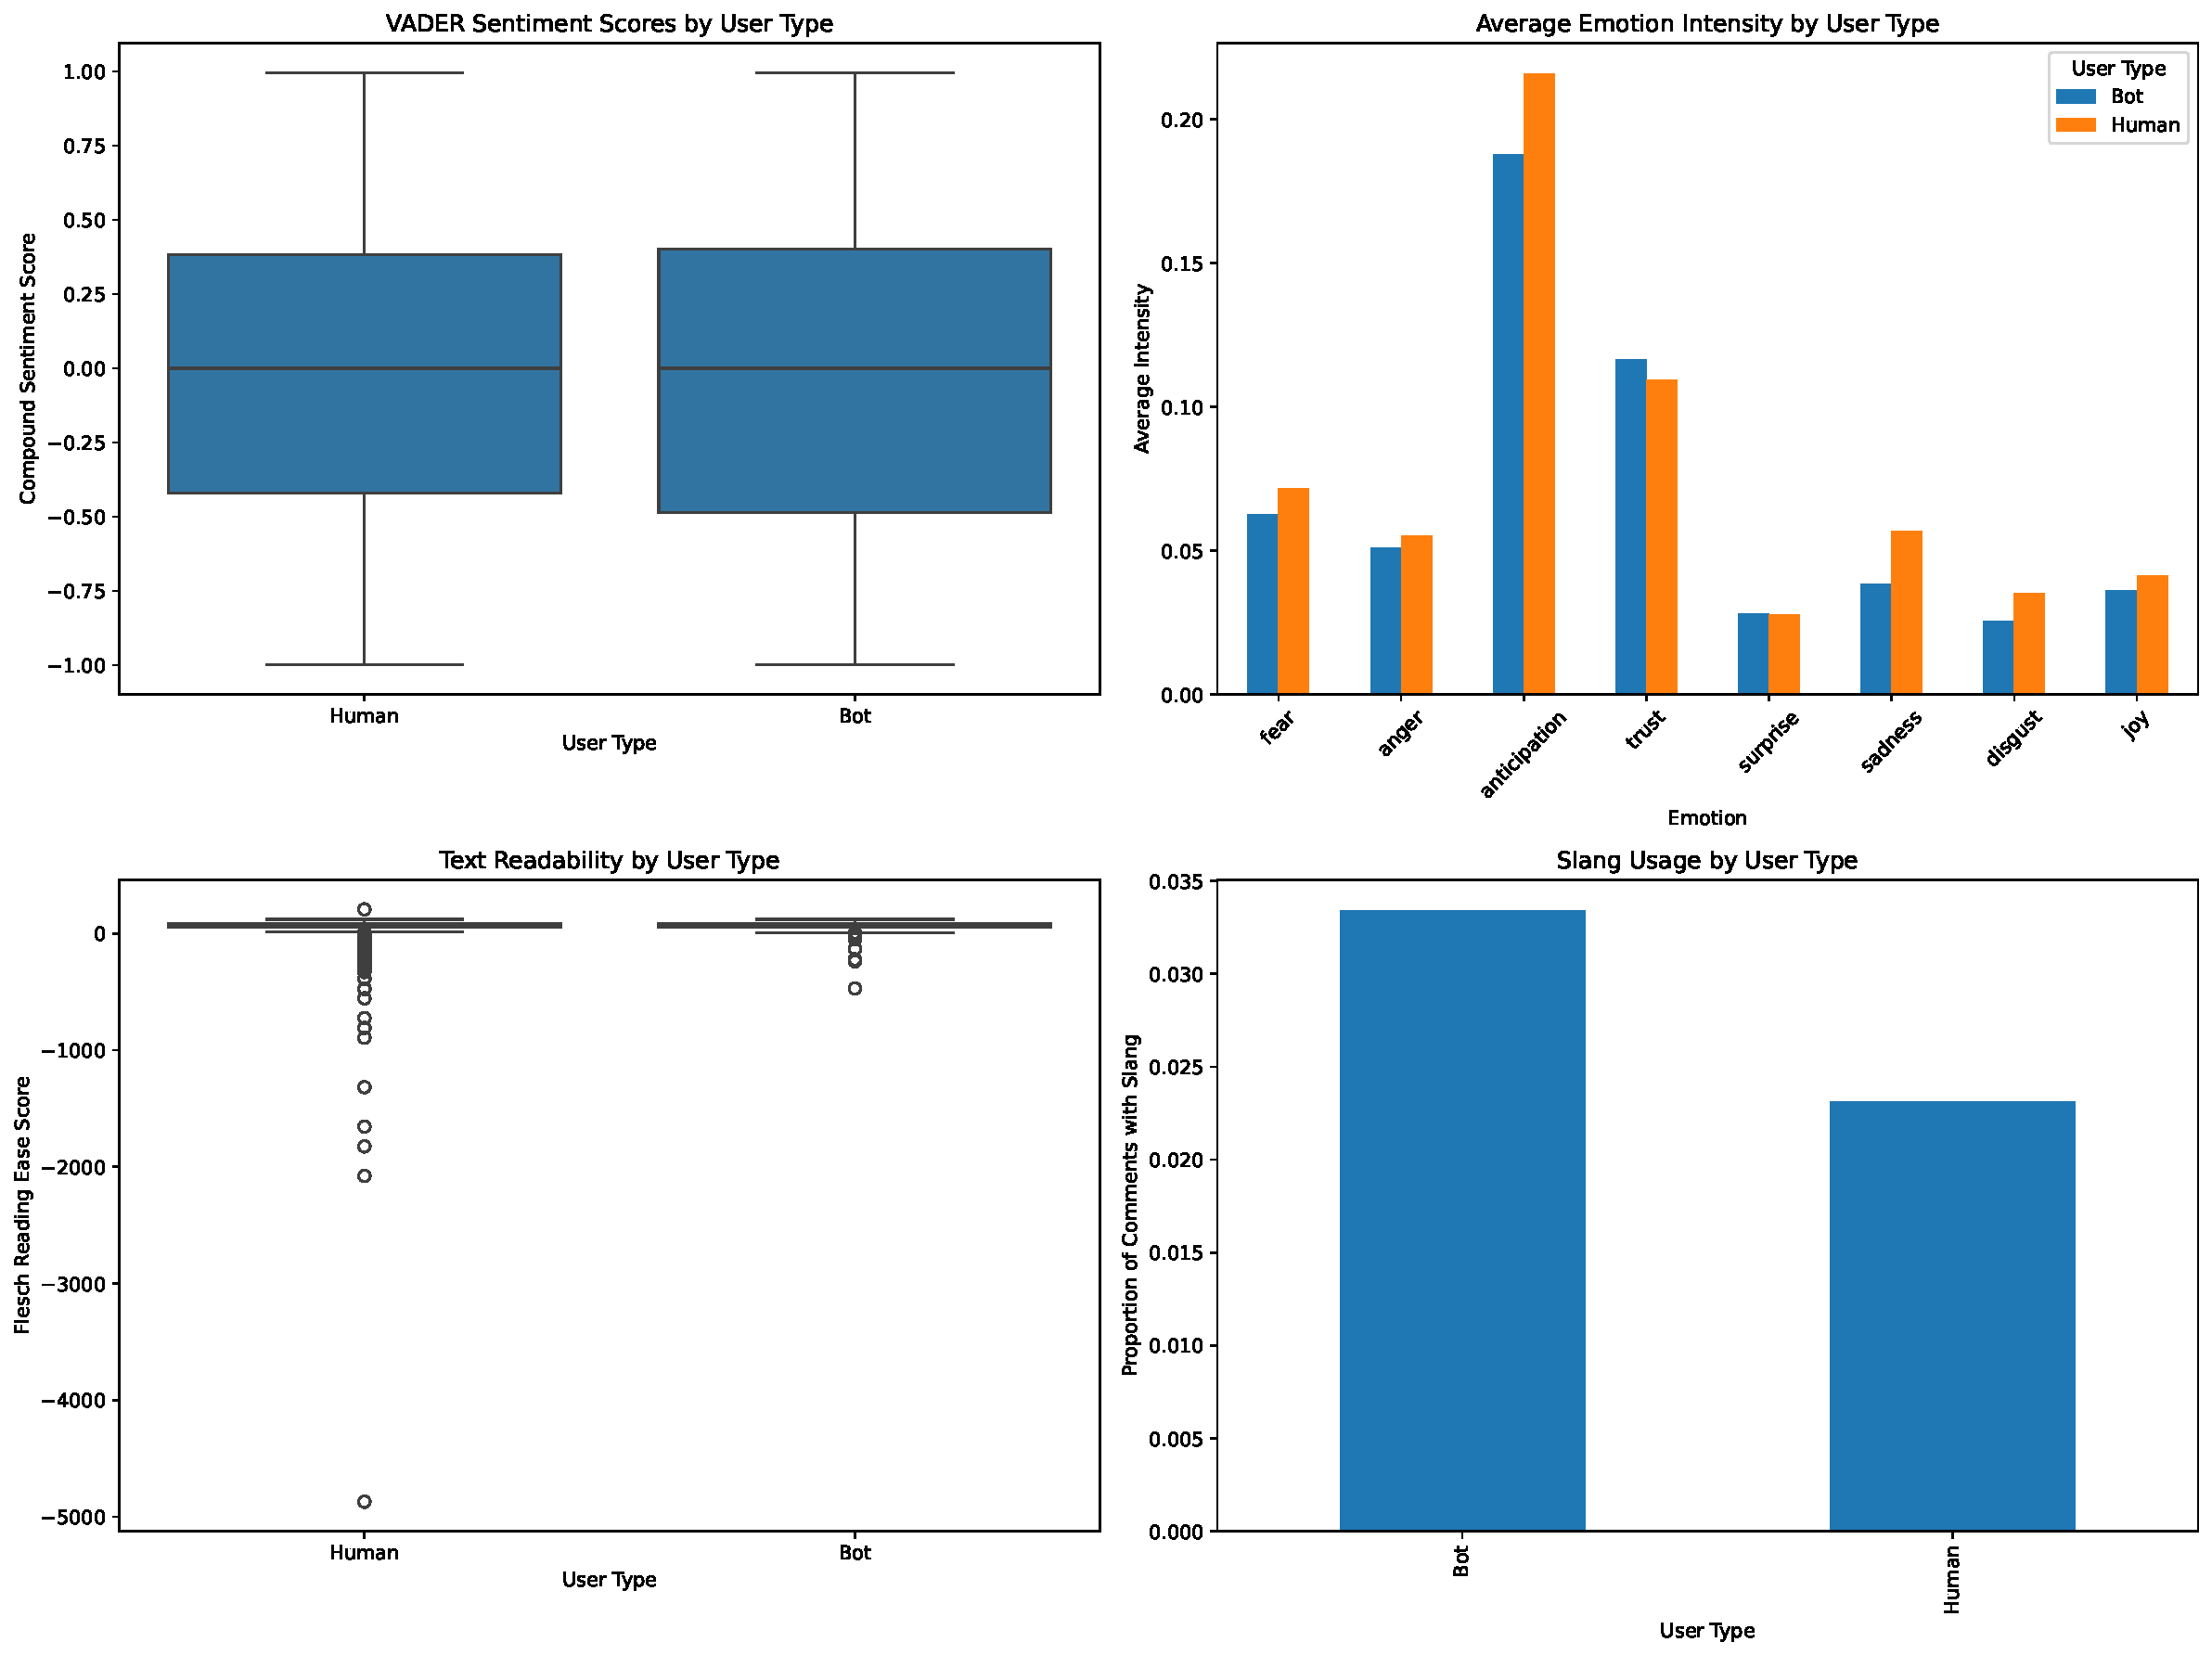
\includegraphics[keepaspectratio]{detecting_bots_on_reddit_code_files/figure-pdf/cell-25-output-1.pdf}}

\pandocbounded{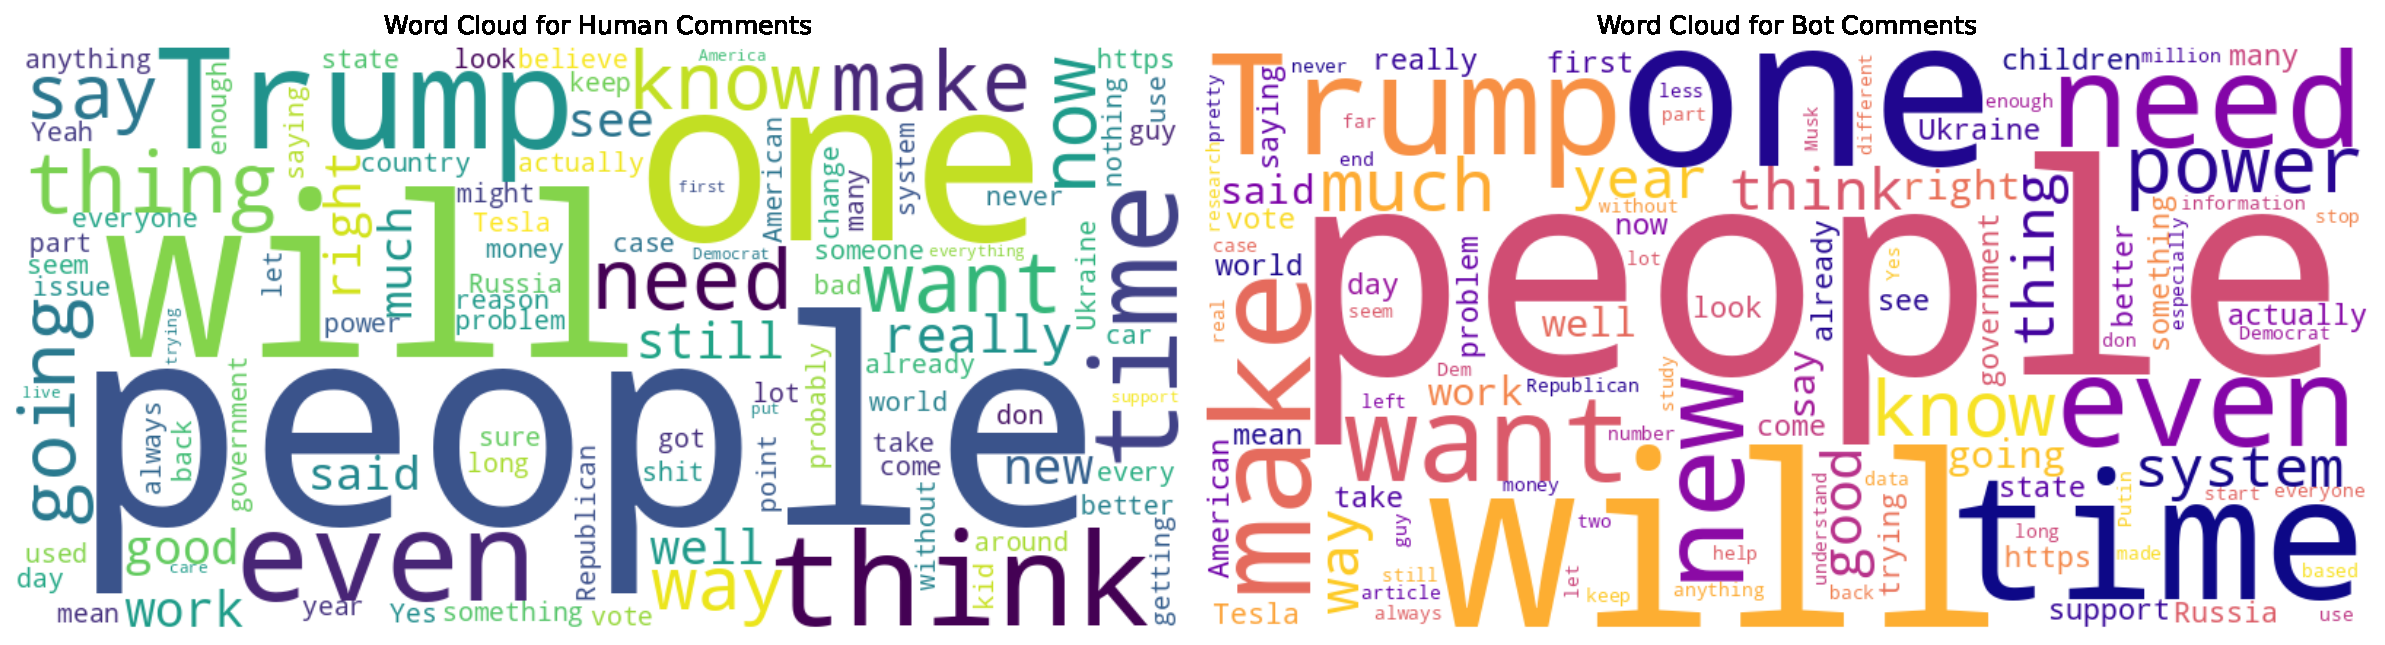
\includegraphics[keepaspectratio]{detecting_bots_on_reddit_code_files/figure-pdf/cell-25-output-2.pdf}}

\pandocbounded{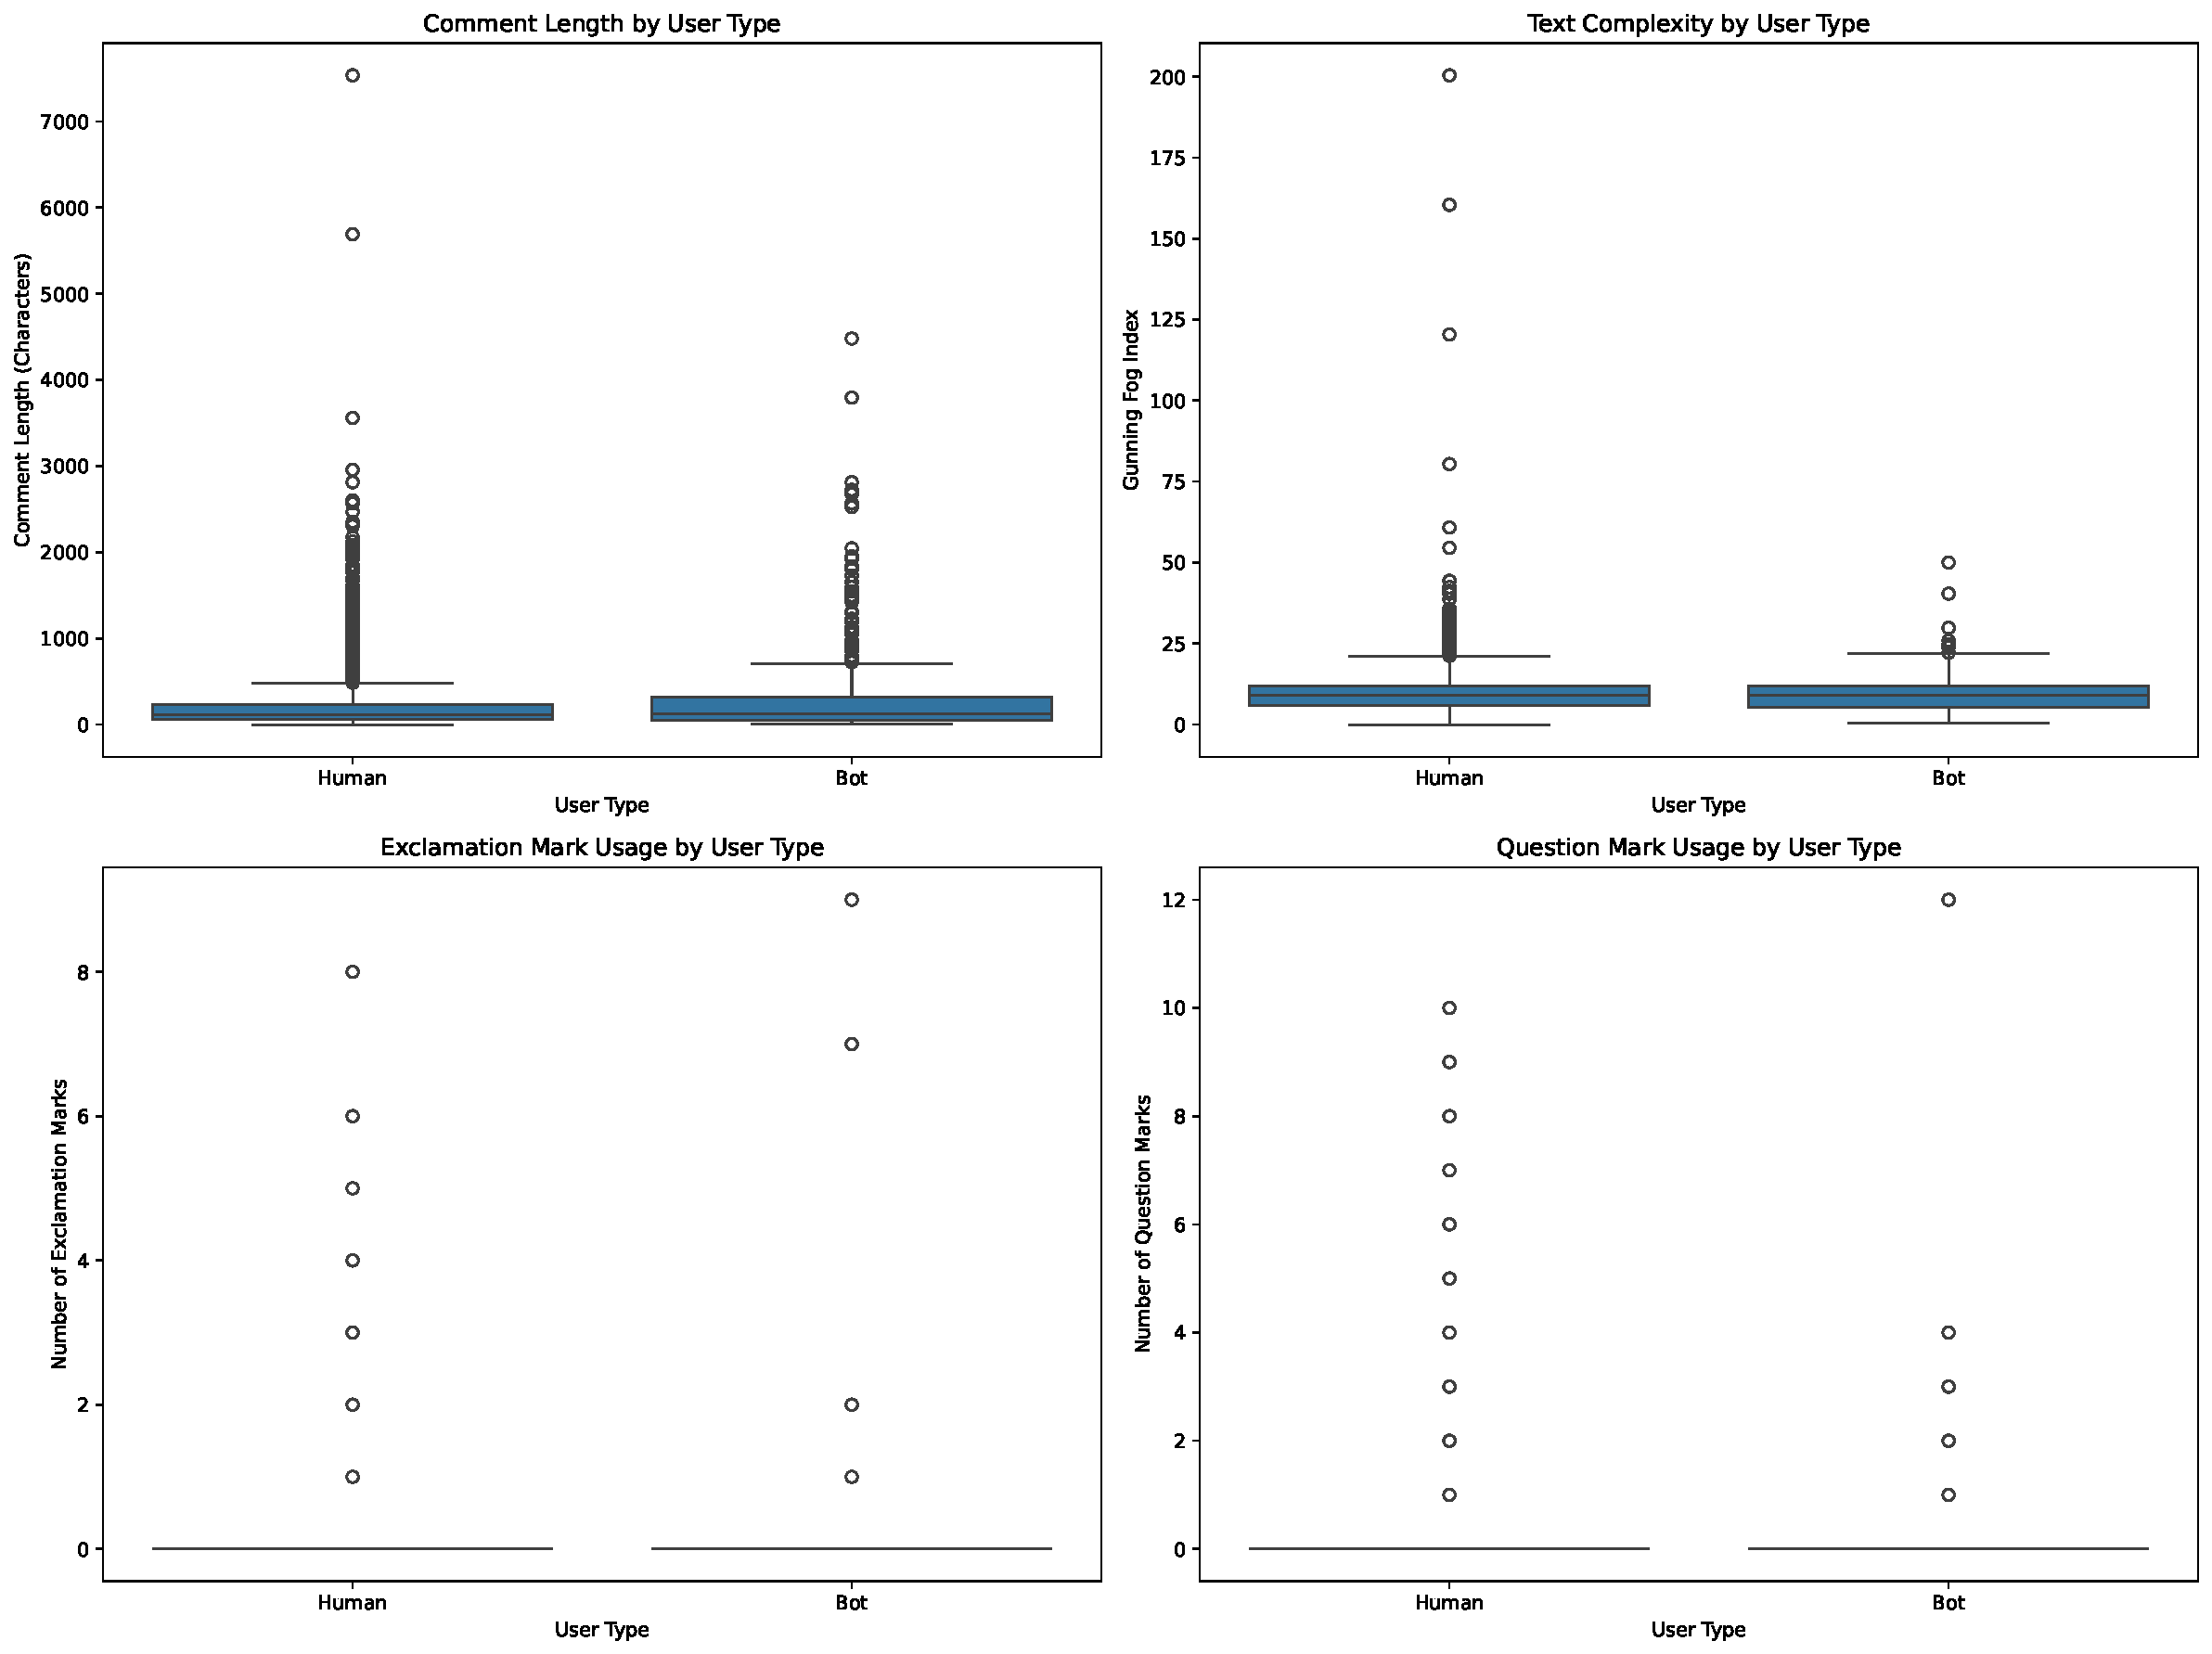
\includegraphics[keepaspectratio]{detecting_bots_on_reddit_code_files/figure-pdf/cell-25-output-3.pdf}}

\begin{verbatim}

=== SENTIMENT ANALYSIS SUMMARY ===

Human Average Sentiment: -0.0173
Bot Average Sentiment: -0.0075

Dominant Human Emotions:
- Anticipation: 0.2158
- Trust: 0.1093
- Fear: 0.0718

Dominant Bot Emotions:
- Anticipation: 0.1877
- Trust: 0.1164
- Fear: 0.0625

Top 10 Common Words in Human Comments:
- people: 1394
- trump: 668
- time: 496
- going: 441
- right: 439
- really: 419
- want: 417
- much: 392
- need: 390
- way: 371

Top 10 Common Words in Bot Comments:
- people: 130
- trump: 59
- time: 46
- power: 43
- much: 42
- right: 41
- need: 40
- want: 38
- many: 37
- way: 37

Linguistic Style Comparison:
Human Average Readability Score: 62.31
Bot Average Readability Score: 63.36
Human Average Complexity Score: 9.55
Bot Average Complexity Score: 9.21
Human Slang Usage Rate: 2.31%
Bot Slang Usage Rate: 3.34%
\end{verbatim}

\begin{Shaded}
\begin{Highlighting}[]
\ImportTok{import}\NormalTok{ pandas }\ImportTok{as}\NormalTok{ pd}
\ImportTok{import}\NormalTok{ numpy }\ImportTok{as}\NormalTok{ np}
\ImportTok{import}\NormalTok{ seaborn }\ImportTok{as}\NormalTok{ sns}
\ImportTok{from}\NormalTok{ nltk.sentiment }\ImportTok{import}\NormalTok{ SentimentIntensityAnalyzer}
\ImportTok{from}\NormalTok{ textblob }\ImportTok{import}\NormalTok{ TextBlob}
\ImportTok{import}\NormalTok{ re}
\ImportTok{from}\NormalTok{ collections }\ImportTok{import}\NormalTok{ Counter}
\ImportTok{from}\NormalTok{ wordcloud }\ImportTok{import}\NormalTok{ WordCloud}
\ImportTok{import}\NormalTok{ nltk}
\ImportTok{from}\NormalTok{ nltk.tokenize }\ImportTok{import}\NormalTok{ word\_tokenize}
\ImportTok{from}\NormalTok{ nltk.corpus }\ImportTok{import}\NormalTok{ stopwords}
\ImportTok{import}\NormalTok{ string}
\ImportTok{from}\NormalTok{ sklearn.feature\_extraction.text }\ImportTok{import}\NormalTok{ CountVectorizer, TfidfVectorizer}
\ImportTok{import}\NormalTok{ textstat}
\ImportTok{from}\NormalTok{ nrclex }\ImportTok{import}\NormalTok{ NRCLex}

\CommentTok{\# Import necessary libraries}
\ImportTok{import}\NormalTok{ matplotlib.pyplot }\ImportTok{as}\NormalTok{ plt}

\CommentTok{\# Download necessary NLTK resources}
\NormalTok{nltk.download(}\StringTok{\textquotesingle{}punkt\textquotesingle{}}\NormalTok{, quiet}\OperatorTok{=}\VariableTok{True}\NormalTok{)}
\NormalTok{nltk.download(}\StringTok{\textquotesingle{}stopwords\textquotesingle{}}\NormalTok{, quiet}\OperatorTok{=}\VariableTok{True}\NormalTok{)}
\NormalTok{nltk.download(}\StringTok{\textquotesingle{}vader\_lexicon\textquotesingle{}}\NormalTok{, quiet}\OperatorTok{=}\VariableTok{True}\NormalTok{)}

\CommentTok{\# Create a filter removing AutoModerator first}
\NormalTok{recent\_user\_comments\_filtered }\OperatorTok{=}\NormalTok{ recent\_user\_comments[recent\_user\_comments[}\StringTok{\textquotesingle{}author\textquotesingle{}}\NormalTok{] }\OperatorTok{!=} \StringTok{\textquotesingle{}AutoModerator\textquotesingle{}}\NormalTok{].copy()}

\CommentTok{\# Create a new column \textquotesingle{}user\_type\textquotesingle{} in recent\_user\_comments\_filtered}
\NormalTok{recent\_user\_comments\_filtered[}\StringTok{\textquotesingle{}user\_type\textquotesingle{}}\NormalTok{] }\OperatorTok{=} \StringTok{\textquotesingle{}Human\textquotesingle{}}  \CommentTok{\# Default to Human}

\CommentTok{\# Merge ml\_features with recent\_user\_comments\_filtered on \textquotesingle{}author\textquotesingle{} to identify bots}
\NormalTok{recent\_user\_comments\_filtered }\OperatorTok{=}\NormalTok{ pd.merge(}
\NormalTok{    recent\_user\_comments\_filtered,}
\NormalTok{    ml\_features[[}\StringTok{\textquotesingle{}comment\_author\textquotesingle{}}\NormalTok{, }\StringTok{\textquotesingle{}possible\_bot\textquotesingle{}}\NormalTok{, }\StringTok{\textquotesingle{}very\_likely\_bot\textquotesingle{}}\NormalTok{]],}
\NormalTok{    left\_on}\OperatorTok{=}\StringTok{\textquotesingle{}author\textquotesingle{}}\NormalTok{,}
\NormalTok{    right\_on}\OperatorTok{=}\StringTok{\textquotesingle{}comment\_author\textquotesingle{}}\NormalTok{,}
\NormalTok{    how}\OperatorTok{=}\StringTok{\textquotesingle{}left\textquotesingle{}}
\NormalTok{)}

\CommentTok{\# Remove duplicate rows based on \textquotesingle{}comment\_id\textquotesingle{}, keeping only the first occurrence}
\NormalTok{recent\_user\_comments\_filtered }\OperatorTok{=}\NormalTok{ recent\_user\_comments\_filtered.drop\_duplicates(subset}\OperatorTok{=}\StringTok{\textquotesingle{}comment\_id\textquotesingle{}}\NormalTok{, keep}\OperatorTok{=}\StringTok{\textquotesingle{}first\textquotesingle{}}\NormalTok{)}

\CommentTok{\# Fill NaN values in \textquotesingle{}possible\_bot\textquotesingle{} and \textquotesingle{}very\_likely\_bot\textquotesingle{} with 0 (not a bot)}
\NormalTok{recent\_user\_comments\_filtered[}\StringTok{\textquotesingle{}possible\_bot\textquotesingle{}}\NormalTok{] }\OperatorTok{=}\NormalTok{ recent\_user\_comments\_filtered[}\StringTok{\textquotesingle{}possible\_bot\textquotesingle{}}\NormalTok{].fillna(}\DecValTok{0}\NormalTok{).astype(}\BuiltInTok{int}\NormalTok{)}
\NormalTok{recent\_user\_comments\_filtered[}\StringTok{\textquotesingle{}very\_likely\_bot\textquotesingle{}}\NormalTok{] }\OperatorTok{=}\NormalTok{ recent\_user\_comments\_filtered[}\StringTok{\textquotesingle{}very\_likely\_bot\textquotesingle{}}\NormalTok{].fillna(}\DecValTok{0}\NormalTok{).astype(}\BuiltInTok{int}\NormalTok{)}

\CommentTok{\# Update \textquotesingle{}user\_type\textquotesingle{} based on bot classifications}
\NormalTok{recent\_user\_comments\_filtered.loc[recent\_user\_comments\_filtered[}\StringTok{\textquotesingle{}possible\_bot\textquotesingle{}}\NormalTok{] }\OperatorTok{==} \DecValTok{1}\NormalTok{, }\StringTok{\textquotesingle{}user\_type\textquotesingle{}}\NormalTok{] }\OperatorTok{=} \StringTok{\textquotesingle{}Bot\textquotesingle{}}
\NormalTok{recent\_user\_comments\_filtered.loc[recent\_user\_comments\_filtered[}\StringTok{\textquotesingle{}very\_likely\_bot\textquotesingle{}}\NormalTok{] }\OperatorTok{==} \DecValTok{1}\NormalTok{, }\StringTok{\textquotesingle{}user\_type\textquotesingle{}}\NormalTok{] }\OperatorTok{=} \StringTok{\textquotesingle{}Bot\textquotesingle{}}

\CommentTok{\# Drop unnecessary columns after the merge}
\NormalTok{recent\_user\_comments\_filtered }\OperatorTok{=}\NormalTok{ recent\_user\_comments\_filtered.drop([}\StringTok{\textquotesingle{}comment\_author\textquotesingle{}}\NormalTok{, }\StringTok{\textquotesingle{}possible\_bot\textquotesingle{}}\NormalTok{, }\StringTok{\textquotesingle{}very\_likely\_bot\textquotesingle{}}\NormalTok{], axis}\OperatorTok{=}\DecValTok{1}\NormalTok{)}

\CommentTok{\# VADER Sentiment Analysis}
\NormalTok{analyzer }\OperatorTok{=}\NormalTok{ SentimentIntensityAnalyzer()}

\CommentTok{\# Add sentiment scores}
\NormalTok{recent\_user\_comments\_filtered[}\StringTok{\textquotesingle{}vader\_compound\textquotesingle{}}\NormalTok{] }\OperatorTok{=}\NormalTok{ recent\_user\_comments\_filtered[}\StringTok{\textquotesingle{}body\textquotesingle{}}\NormalTok{].}\BuiltInTok{apply}\NormalTok{(}\KeywordTok{lambda}\NormalTok{ x: analyzer.polarity\_scores(x)[}\StringTok{\textquotesingle{}compound\textquotesingle{}}\NormalTok{])}
\NormalTok{recent\_user\_comments\_filtered[}\StringTok{\textquotesingle{}vader\_pos\textquotesingle{}}\NormalTok{] }\OperatorTok{=}\NormalTok{ recent\_user\_comments\_filtered[}\StringTok{\textquotesingle{}body\textquotesingle{}}\NormalTok{].}\BuiltInTok{apply}\NormalTok{(}\KeywordTok{lambda}\NormalTok{ x: analyzer.polarity\_scores(x)[}\StringTok{\textquotesingle{}pos\textquotesingle{}}\NormalTok{])}
\NormalTok{recent\_user\_comments\_filtered[}\StringTok{\textquotesingle{}vader\_neg\textquotesingle{}}\NormalTok{] }\OperatorTok{=}\NormalTok{ recent\_user\_comments\_filtered[}\StringTok{\textquotesingle{}body\textquotesingle{}}\NormalTok{].}\BuiltInTok{apply}\NormalTok{(}\KeywordTok{lambda}\NormalTok{ x: analyzer.polarity\_scores(x)[}\StringTok{\textquotesingle{}neg\textquotesingle{}}\NormalTok{])}
\NormalTok{recent\_user\_comments\_filtered[}\StringTok{\textquotesingle{}vader\_neu\textquotesingle{}}\NormalTok{] }\OperatorTok{=}\NormalTok{ recent\_user\_comments\_filtered[}\StringTok{\textquotesingle{}body\textquotesingle{}}\NormalTok{].}\BuiltInTok{apply}\NormalTok{(}\KeywordTok{lambda}\NormalTok{ x: analyzer.polarity\_scores(x)[}\StringTok{\textquotesingle{}neu\textquotesingle{}}\NormalTok{])}

\CommentTok{\# Calculate text complexity metrics}
\NormalTok{recent\_user\_comments\_filtered[}\StringTok{\textquotesingle{}comment\_length\textquotesingle{}}\NormalTok{] }\OperatorTok{=}\NormalTok{ recent\_user\_comments\_filtered[}\StringTok{\textquotesingle{}body\textquotesingle{}}\NormalTok{].}\BuiltInTok{apply}\NormalTok{(}\BuiltInTok{len}\NormalTok{)}
\NormalTok{recent\_user\_comments\_filtered[}\StringTok{\textquotesingle{}readability\_score\textquotesingle{}}\NormalTok{] }\OperatorTok{=}\NormalTok{ recent\_user\_comments\_filtered[}\StringTok{\textquotesingle{}body\textquotesingle{}}\NormalTok{].}\BuiltInTok{apply}\NormalTok{(}\KeywordTok{lambda}\NormalTok{ x: textstat.flesch\_reading\_ease(x))}
\NormalTok{recent\_user\_comments\_filtered[}\StringTok{\textquotesingle{}complexity\_score\textquotesingle{}}\NormalTok{] }\OperatorTok{=}\NormalTok{ recent\_user\_comments\_filtered[}\StringTok{\textquotesingle{}body\textquotesingle{}}\NormalTok{].}\BuiltInTok{apply}\NormalTok{(}\KeywordTok{lambda}\NormalTok{ x: textstat.gunning\_fog(x))}

\CommentTok{\# Function to detect slang or informal language}
\KeywordTok{def}\NormalTok{ contains\_slang(text):}
    \CommentTok{\# Simple slang detection based on common patterns}
\NormalTok{    slang\_patterns }\OperatorTok{=}\NormalTok{ [}\VerbatimStringTok{r\textquotesingle{}\textbackslash{}blol\textbackslash{}b\textquotesingle{}}\NormalTok{, }\VerbatimStringTok{r\textquotesingle{}\textbackslash{}bomg\textbackslash{}b\textquotesingle{}}\NormalTok{, }\VerbatimStringTok{r\textquotesingle{}\textbackslash{}bbtw\textbackslash{}b\textquotesingle{}}\NormalTok{, }\VerbatimStringTok{r\textquotesingle{}\textbackslash{}bidk\textbackslash{}b\textquotesingle{}}\NormalTok{, }\VerbatimStringTok{r\textquotesingle{}\textbackslash{}bimo\textbackslash{}b\textquotesingle{}}\NormalTok{, }\VerbatimStringTok{r\textquotesingle{}\textbackslash{}bfyi\textbackslash{}b\textquotesingle{}}\NormalTok{, }
                      \VerbatimStringTok{r\textquotesingle{}\textbackslash{}bsmh\textbackslash{}b\textquotesingle{}}\NormalTok{, }\VerbatimStringTok{r\textquotesingle{}\textbackslash{}bwtf\textbackslash{}b\textquotesingle{}}\NormalTok{, }\VerbatimStringTok{r\textquotesingle{}\textbackslash{}baf\textbackslash{}b\textquotesingle{}}\NormalTok{, }\VerbatimStringTok{r\textquotesingle{}\textbackslash{}bfr\textbackslash{}b\textquotesingle{}}\NormalTok{, }\VerbatimStringTok{r\textquotesingle{}\textbackslash{}byolo\textbackslash{}b\textquotesingle{}}\NormalTok{, }\VerbatimStringTok{r\textquotesingle{}\textbackslash{}btbh\textbackslash{}b\textquotesingle{}}\NormalTok{,}
                      \VerbatimStringTok{r\textquotesingle{}\textbackslash{}brofl\textbackslash{}b\textquotesingle{}}\NormalTok{, }\VerbatimStringTok{r\textquotesingle{}\textbackslash{}blmao\textbackslash{}b\textquotesingle{}}\NormalTok{, }\VerbatimStringTok{r\textquotesingle{}\textbackslash{}blmfao\textbackslash{}b\textquotesingle{}}\NormalTok{, }\VerbatimStringTok{r\textquotesingle{}\textbackslash{}bbrb\textbackslash{}b\textquotesingle{}}\NormalTok{, }\VerbatimStringTok{r\textquotesingle{}\textbackslash{}bafaik\textbackslash{}b\textquotesingle{}}\NormalTok{,}
                      \VerbatimStringTok{r\textquotesingle{}\textbackslash{}bftw\textbackslash{}b\textquotesingle{}}\NormalTok{, }\VerbatimStringTok{r\textquotesingle{}\textbackslash{}bfml\textbackslash{}b\textquotesingle{}}\NormalTok{, }\VerbatimStringTok{r\textquotesingle{}\textbackslash{}bomfg\textbackslash{}b\textquotesingle{}}\NormalTok{, }\VerbatimStringTok{r\textquotesingle{}\textbackslash{}bidc\textbackslash{}b\textquotesingle{}}\NormalTok{, }\VerbatimStringTok{r\textquotesingle{}\textbackslash{}bimho\textbackslash{}b\textquotesingle{}}\NormalTok{]}
    
    \ControlFlowTok{for}\NormalTok{ pattern }\KeywordTok{in}\NormalTok{ slang\_patterns:}
        \ControlFlowTok{if}\NormalTok{ re.search(pattern, text.lower()):}
            \ControlFlowTok{return} \DecValTok{1}
    \ControlFlowTok{return} \DecValTok{0}

\CommentTok{\# Function to count exclamation and question marks}
\KeywordTok{def}\NormalTok{ count\_punctuation(text):}
\NormalTok{    exclamation\_count }\OperatorTok{=}\NormalTok{ text.count(}\StringTok{\textquotesingle{}!\textquotesingle{}}\NormalTok{)}
\NormalTok{    question\_count }\OperatorTok{=}\NormalTok{ text.count(}\StringTok{\textquotesingle{}?\textquotesingle{}}\NormalTok{)}
    \ControlFlowTok{return}\NormalTok{ exclamation\_count, question\_count}

\CommentTok{\# Apply the slang detection and punctuation counting}
\NormalTok{recent\_user\_comments\_filtered[}\StringTok{\textquotesingle{}contains\_slang\textquotesingle{}}\NormalTok{] }\OperatorTok{=}\NormalTok{ recent\_user\_comments\_filtered[}\StringTok{\textquotesingle{}body\textquotesingle{}}\NormalTok{].}\BuiltInTok{apply}\NormalTok{(contains\_slang)}
\NormalTok{recent\_user\_comments\_filtered[}\StringTok{\textquotesingle{}exclamation\_count\textquotesingle{}}\NormalTok{] }\OperatorTok{=}\NormalTok{ recent\_user\_comments\_filtered[}\StringTok{\textquotesingle{}body\textquotesingle{}}\NormalTok{].}\BuiltInTok{apply}\NormalTok{(}\KeywordTok{lambda}\NormalTok{ x: count\_punctuation(x)[}\DecValTok{0}\NormalTok{])}
\NormalTok{recent\_user\_comments\_filtered[}\StringTok{\textquotesingle{}question\_count\textquotesingle{}}\NormalTok{] }\OperatorTok{=}\NormalTok{ recent\_user\_comments\_filtered[}\StringTok{\textquotesingle{}body\textquotesingle{}}\NormalTok{].}\BuiltInTok{apply}\NormalTok{(}\KeywordTok{lambda}\NormalTok{ x: count\_punctuation(x)[}\DecValTok{1}\NormalTok{])}

\CommentTok{\# Emotion Detection using NRCLex}
\KeywordTok{def}\NormalTok{ extract\_emotions(text):}
\NormalTok{    emotion\_scores }\OperatorTok{=}\NormalTok{ NRCLex(text).affect\_frequencies}
    \ControlFlowTok{return}\NormalTok{ emotion\_scores}

\CommentTok{\# Extract a sample due to computational constraints}
\NormalTok{sample\_size }\OperatorTok{=} \BuiltInTok{min}\NormalTok{(}\DecValTok{1000}\NormalTok{, }\BuiltInTok{len}\NormalTok{(recent\_user\_comments\_filtered))}
\NormalTok{emotions\_sample }\OperatorTok{=}\NormalTok{ recent\_user\_comments\_filtered.sample(sample\_size, random\_state}\OperatorTok{=}\DecValTok{42}\NormalTok{)}

\CommentTok{\# Apply emotion extraction}
\NormalTok{emotions\_df }\OperatorTok{=}\NormalTok{ pd.DataFrame([extract\_emotions(text) }\ControlFlowTok{for}\NormalTok{ text }\KeywordTok{in}\NormalTok{ emotions\_sample[}\StringTok{\textquotesingle{}body\textquotesingle{}}\NormalTok{]])}
\NormalTok{emotions\_sample }\OperatorTok{=}\NormalTok{ pd.concat([emotions\_sample.reset\_index(drop}\OperatorTok{=}\VariableTok{True}\NormalTok{), emotions\_df.reset\_index(drop}\OperatorTok{=}\VariableTok{True}\NormalTok{)], axis}\OperatorTok{=}\DecValTok{1}\NormalTok{)}

\CommentTok{\# Create visualization for sentiment comparison}
\NormalTok{plt.figure(figsize}\OperatorTok{=}\NormalTok{(}\DecValTok{16}\NormalTok{, }\DecValTok{12}\NormalTok{))}

\CommentTok{\# 1. VADER Sentiment Distribution}
\NormalTok{plt.subplot(}\DecValTok{2}\NormalTok{, }\DecValTok{2}\NormalTok{, }\DecValTok{1}\NormalTok{)}
\NormalTok{sns.boxplot(x}\OperatorTok{=}\StringTok{\textquotesingle{}user\_type\textquotesingle{}}\NormalTok{, y}\OperatorTok{=}\StringTok{\textquotesingle{}vader\_compound\textquotesingle{}}\NormalTok{, data}\OperatorTok{=}\NormalTok{recent\_user\_comments\_filtered)}
\NormalTok{plt.title(}\StringTok{\textquotesingle{}VADER Sentiment Scores by User Type\textquotesingle{}}\NormalTok{)}
\NormalTok{plt.xlabel(}\StringTok{\textquotesingle{}User Type\textquotesingle{}}\NormalTok{)}
\NormalTok{plt.ylabel(}\StringTok{\textquotesingle{}Compound Sentiment Score\textquotesingle{}}\NormalTok{)}

\CommentTok{\# 2. Emotion Comparison}
\NormalTok{plt.subplot(}\DecValTok{2}\NormalTok{, }\DecValTok{2}\NormalTok{, }\DecValTok{2}\NormalTok{)}
\NormalTok{emotion\_cols }\OperatorTok{=}\NormalTok{ [}\StringTok{\textquotesingle{}fear\textquotesingle{}}\NormalTok{, }\StringTok{\textquotesingle{}anger\textquotesingle{}}\NormalTok{, }\StringTok{\textquotesingle{}anticipation\textquotesingle{}}\NormalTok{, }\StringTok{\textquotesingle{}trust\textquotesingle{}}\NormalTok{, }\StringTok{\textquotesingle{}surprise\textquotesingle{}}\NormalTok{, }\StringTok{\textquotesingle{}sadness\textquotesingle{}}\NormalTok{, }\StringTok{\textquotesingle{}disgust\textquotesingle{}}\NormalTok{, }\StringTok{\textquotesingle{}joy\textquotesingle{}}\NormalTok{]}
\NormalTok{emotions\_by\_type }\OperatorTok{=}\NormalTok{ emotions\_sample.groupby(}\StringTok{\textquotesingle{}user\_type\textquotesingle{}}\NormalTok{)[emotion\_cols].mean()}
\NormalTok{emotions\_by\_type.T.plot(kind}\OperatorTok{=}\StringTok{\textquotesingle{}bar\textquotesingle{}}\NormalTok{, ax}\OperatorTok{=}\NormalTok{plt.gca())}
\NormalTok{plt.title(}\StringTok{\textquotesingle{}Average Emotion Intensity by User Type\textquotesingle{}}\NormalTok{)}
\NormalTok{plt.xlabel(}\StringTok{\textquotesingle{}Emotion\textquotesingle{}}\NormalTok{)}
\NormalTok{plt.ylabel(}\StringTok{\textquotesingle{}Average Intensity\textquotesingle{}}\NormalTok{)}
\NormalTok{plt.xticks(rotation}\OperatorTok{=}\DecValTok{45}\NormalTok{)}
\NormalTok{plt.legend(title}\OperatorTok{=}\StringTok{\textquotesingle{}User Type\textquotesingle{}}\NormalTok{)}

\CommentTok{\# 3. Text Complexity}
\NormalTok{plt.subplot(}\DecValTok{2}\NormalTok{, }\DecValTok{2}\NormalTok{, }\DecValTok{3}\NormalTok{)}
\NormalTok{sns.boxplot(x}\OperatorTok{=}\StringTok{\textquotesingle{}user\_type\textquotesingle{}}\NormalTok{, y}\OperatorTok{=}\StringTok{\textquotesingle{}readability\_score\textquotesingle{}}\NormalTok{, data}\OperatorTok{=}\NormalTok{recent\_user\_comments\_filtered)}
\NormalTok{plt.title(}\StringTok{\textquotesingle{}Text Readability by User Type\textquotesingle{}}\NormalTok{)}
\NormalTok{plt.xlabel(}\StringTok{\textquotesingle{}User Type\textquotesingle{}}\NormalTok{)}
\NormalTok{plt.ylabel(}\StringTok{\textquotesingle{}Flesch Reading Ease Score\textquotesingle{}}\NormalTok{)}

\CommentTok{\# 4. Slang Usage}
\NormalTok{plt.subplot(}\DecValTok{2}\NormalTok{, }\DecValTok{2}\NormalTok{, }\DecValTok{4}\NormalTok{)}
\NormalTok{slang\_by\_type }\OperatorTok{=}\NormalTok{ recent\_user\_comments\_filtered.groupby(}\StringTok{\textquotesingle{}user\_type\textquotesingle{}}\NormalTok{)[}\StringTok{\textquotesingle{}contains\_slang\textquotesingle{}}\NormalTok{].mean()}
\NormalTok{slang\_by\_type.plot(kind}\OperatorTok{=}\StringTok{\textquotesingle{}bar\textquotesingle{}}\NormalTok{, ax}\OperatorTok{=}\NormalTok{plt.gca())}
\NormalTok{plt.title(}\StringTok{\textquotesingle{}Slang Usage by User Type\textquotesingle{}}\NormalTok{)}
\NormalTok{plt.xlabel(}\StringTok{\textquotesingle{}User Type\textquotesingle{}}\NormalTok{)}
\NormalTok{plt.ylabel(}\StringTok{\textquotesingle{}Proportion of Comments with Slang\textquotesingle{}}\NormalTok{)}

\NormalTok{plt.tight\_layout()}
\NormalTok{plt.show()}

\CommentTok{\# Extract common words by user type}
\KeywordTok{def}\NormalTok{ get\_common\_words(texts, n}\OperatorTok{=}\DecValTok{20}\NormalTok{):}
    \CommentTok{\# Tokenize and clean}
\NormalTok{    stop\_words }\OperatorTok{=} \BuiltInTok{set}\NormalTok{(stopwords.words(}\StringTok{\textquotesingle{}english\textquotesingle{}}\NormalTok{))}
\NormalTok{    stop\_words.update([}\StringTok{\textquotesingle{}would\textquotesingle{}}\NormalTok{, }\StringTok{\textquotesingle{}could\textquotesingle{}}\NormalTok{, }\StringTok{\textquotesingle{}also\textquotesingle{}}\NormalTok{, }\StringTok{\textquotesingle{}one\textquotesingle{}}\NormalTok{, }\StringTok{\textquotesingle{}like\textquotesingle{}}\NormalTok{, }\StringTok{\textquotesingle{}get\textquotesingle{}}\NormalTok{, }\StringTok{\textquotesingle{}even\textquotesingle{}}\NormalTok{, }\StringTok{\textquotesingle{}say\textquotesingle{}}\NormalTok{, }\StringTok{\textquotesingle{}said\textquotesingle{}}\NormalTok{, }\StringTok{\textquotesingle{}make\textquotesingle{}}\NormalTok{, }\StringTok{\textquotesingle{}think\textquotesingle{}}\NormalTok{, }\StringTok{\textquotesingle{}know\textquotesingle{}}\NormalTok{])}
    
\NormalTok{    words }\OperatorTok{=}\NormalTok{ []}
    \ControlFlowTok{for}\NormalTok{ text }\KeywordTok{in}\NormalTok{ texts:}
\NormalTok{        tokens }\OperatorTok{=}\NormalTok{ word\_tokenize(text.lower())}
        \CommentTok{\# Remove stopwords, punctuation, and non{-}alphabetic tokens}
\NormalTok{        words.extend([word }\ControlFlowTok{for}\NormalTok{ word }\KeywordTok{in}\NormalTok{ tokens }\ControlFlowTok{if}\NormalTok{ word }\KeywordTok{not} \KeywordTok{in}\NormalTok{ stop\_words }
                     \KeywordTok{and}\NormalTok{ word }\KeywordTok{not} \KeywordTok{in}\NormalTok{ string.punctuation }
                     \KeywordTok{and}\NormalTok{ word.isalpha() }
                     \KeywordTok{and} \BuiltInTok{len}\NormalTok{(word) }\OperatorTok{\textgreater{}} \DecValTok{2}\NormalTok{])}
    
    \ControlFlowTok{return}\NormalTok{ Counter(words).most\_common(n)}

\CommentTok{\# Get most common words for humans and bots}
\NormalTok{human\_texts }\OperatorTok{=}\NormalTok{ recent\_user\_comments\_filtered[recent\_user\_comments\_filtered[}\StringTok{\textquotesingle{}user\_type\textquotesingle{}}\NormalTok{] }\OperatorTok{==} \StringTok{\textquotesingle{}Human\textquotesingle{}}\NormalTok{][}\StringTok{\textquotesingle{}body\textquotesingle{}}\NormalTok{].tolist()}
\NormalTok{bot\_texts }\OperatorTok{=}\NormalTok{ recent\_user\_comments\_filtered[recent\_user\_comments\_filtered[}\StringTok{\textquotesingle{}user\_type\textquotesingle{}}\NormalTok{] }\OperatorTok{==} \StringTok{\textquotesingle{}Bot\textquotesingle{}}\NormalTok{][}\StringTok{\textquotesingle{}body\textquotesingle{}}\NormalTok{].tolist()}

\NormalTok{human\_common\_words }\OperatorTok{=}\NormalTok{ get\_common\_words(human\_texts)}
\NormalTok{bot\_common\_words }\OperatorTok{=}\NormalTok{ get\_common\_words(bot\_texts)}

\CommentTok{\# Create word clouds}
\NormalTok{plt.figure(figsize}\OperatorTok{=}\NormalTok{(}\DecValTok{16}\NormalTok{, }\DecValTok{8}\NormalTok{))}

\CommentTok{\# Word cloud for humans}
\NormalTok{plt.subplot(}\DecValTok{1}\NormalTok{, }\DecValTok{2}\NormalTok{, }\DecValTok{1}\NormalTok{)}
\NormalTok{human\_wordcloud }\OperatorTok{=}\NormalTok{ WordCloud(width}\OperatorTok{=}\DecValTok{800}\NormalTok{, height}\OperatorTok{=}\DecValTok{400}\NormalTok{, background\_color}\OperatorTok{=}\StringTok{\textquotesingle{}white\textquotesingle{}}\NormalTok{, }
\NormalTok{                           max\_words}\OperatorTok{=}\DecValTok{100}\NormalTok{, colormap}\OperatorTok{=}\StringTok{\textquotesingle{}viridis\textquotesingle{}}\NormalTok{, min\_word\_length}\OperatorTok{=}\DecValTok{3}\NormalTok{).generate(}\StringTok{\textquotesingle{} \textquotesingle{}}\NormalTok{.join(human\_texts))}
\NormalTok{plt.imshow(human\_wordcloud, interpolation}\OperatorTok{=}\StringTok{\textquotesingle{}bilinear\textquotesingle{}}\NormalTok{)}
\NormalTok{plt.title(}\StringTok{\textquotesingle{}Word Cloud for Human Comments\textquotesingle{}}\NormalTok{)}
\NormalTok{plt.axis(}\StringTok{\textquotesingle{}off\textquotesingle{}}\NormalTok{)}

\CommentTok{\# Word cloud for bots}
\NormalTok{plt.subplot(}\DecValTok{1}\NormalTok{, }\DecValTok{2}\NormalTok{, }\DecValTok{2}\NormalTok{)}
\NormalTok{bot\_wordcloud }\OperatorTok{=}\NormalTok{ WordCloud(width}\OperatorTok{=}\DecValTok{800}\NormalTok{, height}\OperatorTok{=}\DecValTok{400}\NormalTok{, background\_color}\OperatorTok{=}\StringTok{\textquotesingle{}white\textquotesingle{}}\NormalTok{, }
\NormalTok{                         max\_words}\OperatorTok{=}\DecValTok{100}\NormalTok{, colormap}\OperatorTok{=}\StringTok{\textquotesingle{}plasma\textquotesingle{}}\NormalTok{, min\_word\_length}\OperatorTok{=}\DecValTok{3}\NormalTok{).generate(}\StringTok{\textquotesingle{} \textquotesingle{}}\NormalTok{.join(bot\_texts))}
\NormalTok{plt.imshow(bot\_wordcloud, interpolation}\OperatorTok{=}\StringTok{\textquotesingle{}bilinear\textquotesingle{}}\NormalTok{)}
\NormalTok{plt.title(}\StringTok{\textquotesingle{}Word Cloud for Bot Comments\textquotesingle{}}\NormalTok{)}
\NormalTok{plt.axis(}\StringTok{\textquotesingle{}off\textquotesingle{}}\NormalTok{)}

\NormalTok{plt.tight\_layout()}
\NormalTok{plt.show()}

\CommentTok{\# Compare linguistic style metrics}
\NormalTok{plt.figure(figsize}\OperatorTok{=}\NormalTok{(}\DecValTok{16}\NormalTok{, }\DecValTok{12}\NormalTok{))}

\CommentTok{\# 1. Comment Length Comparison}
\NormalTok{plt.subplot(}\DecValTok{2}\NormalTok{, }\DecValTok{2}\NormalTok{, }\DecValTok{1}\NormalTok{)}
\NormalTok{sns.boxplot(x}\OperatorTok{=}\StringTok{\textquotesingle{}user\_type\textquotesingle{}}\NormalTok{, y}\OperatorTok{=}\StringTok{\textquotesingle{}comment\_length\textquotesingle{}}\NormalTok{, data}\OperatorTok{=}\NormalTok{recent\_user\_comments\_filtered)}
\NormalTok{plt.title(}\StringTok{\textquotesingle{}Comment Length by User Type\textquotesingle{}}\NormalTok{)}
\NormalTok{plt.xlabel(}\StringTok{\textquotesingle{}User Type\textquotesingle{}}\NormalTok{)}
\NormalTok{plt.ylabel(}\StringTok{\textquotesingle{}Comment Length (Characters)\textquotesingle{}}\NormalTok{)}

\CommentTok{\# 2. Complexity Score Comparison}
\NormalTok{plt.subplot(}\DecValTok{2}\NormalTok{, }\DecValTok{2}\NormalTok{, }\DecValTok{2}\NormalTok{)}
\NormalTok{sns.boxplot(x}\OperatorTok{=}\StringTok{\textquotesingle{}user\_type\textquotesingle{}}\NormalTok{, y}\OperatorTok{=}\StringTok{\textquotesingle{}complexity\_score\textquotesingle{}}\NormalTok{, data}\OperatorTok{=}\NormalTok{recent\_user\_comments\_filtered)}
\NormalTok{plt.title(}\StringTok{\textquotesingle{}Text Complexity by User Type\textquotesingle{}}\NormalTok{)}
\NormalTok{plt.xlabel(}\StringTok{\textquotesingle{}User Type\textquotesingle{}}\NormalTok{)}
\NormalTok{plt.ylabel(}\StringTok{\textquotesingle{}Gunning Fog Index\textquotesingle{}}\NormalTok{)}

\CommentTok{\# 3. Exclamation Mark Usage}
\NormalTok{plt.subplot(}\DecValTok{2}\NormalTok{, }\DecValTok{2}\NormalTok{, }\DecValTok{3}\NormalTok{)}
\NormalTok{sns.boxplot(x}\OperatorTok{=}\StringTok{\textquotesingle{}user\_type\textquotesingle{}}\NormalTok{, y}\OperatorTok{=}\StringTok{\textquotesingle{}exclamation\_count\textquotesingle{}}\NormalTok{, data}\OperatorTok{=}\NormalTok{recent\_user\_comments\_filtered)}
\NormalTok{plt.title(}\StringTok{\textquotesingle{}Exclamation Mark Usage by User Type\textquotesingle{}}\NormalTok{)}
\NormalTok{plt.xlabel(}\StringTok{\textquotesingle{}User Type\textquotesingle{}}\NormalTok{)}
\NormalTok{plt.ylabel(}\StringTok{\textquotesingle{}Number of Exclamation Marks\textquotesingle{}}\NormalTok{)}

\CommentTok{\# 4. Question Mark Usage}
\NormalTok{plt.subplot(}\DecValTok{2}\NormalTok{, }\DecValTok{2}\NormalTok{, }\DecValTok{4}\NormalTok{)}
\NormalTok{sns.boxplot(x}\OperatorTok{=}\StringTok{\textquotesingle{}user\_type\textquotesingle{}}\NormalTok{, y}\OperatorTok{=}\StringTok{\textquotesingle{}question\_count\textquotesingle{}}\NormalTok{, data}\OperatorTok{=}\NormalTok{recent\_user\_comments\_filtered)}
\NormalTok{plt.title(}\StringTok{\textquotesingle{}Question Mark Usage by User Type\textquotesingle{}}\NormalTok{)}
\NormalTok{plt.xlabel(}\StringTok{\textquotesingle{}User Type\textquotesingle{}}\NormalTok{)}
\NormalTok{plt.ylabel(}\StringTok{\textquotesingle{}Number of Question Marks\textquotesingle{}}\NormalTok{)}

\NormalTok{plt.tight\_layout()}
\NormalTok{plt.show()}

\CommentTok{\# Generate summary report}
\NormalTok{human\_sentiment }\OperatorTok{=}\NormalTok{ recent\_user\_comments\_filtered[recent\_user\_comments\_filtered[}\StringTok{\textquotesingle{}user\_type\textquotesingle{}}\NormalTok{] }\OperatorTok{==} \StringTok{\textquotesingle{}Human\textquotesingle{}}\NormalTok{][}\StringTok{\textquotesingle{}vader\_compound\textquotesingle{}}\NormalTok{].mean()}
\NormalTok{bot\_sentiment }\OperatorTok{=}\NormalTok{ recent\_user\_comments\_filtered[recent\_user\_comments\_filtered[}\StringTok{\textquotesingle{}user\_type\textquotesingle{}}\NormalTok{] }\OperatorTok{==} \StringTok{\textquotesingle{}Bot\textquotesingle{}}\NormalTok{][}\StringTok{\textquotesingle{}vader\_compound\textquotesingle{}}\NormalTok{].mean()}

\NormalTok{human\_emotions }\OperatorTok{=}\NormalTok{ emotions\_sample[emotions\_sample[}\StringTok{\textquotesingle{}user\_type\textquotesingle{}}\NormalTok{] }\OperatorTok{==} \StringTok{\textquotesingle{}Human\textquotesingle{}}\NormalTok{][emotion\_cols].mean()}
\NormalTok{bot\_emotions }\OperatorTok{=}\NormalTok{ emotions\_sample[emotions\_sample[}\StringTok{\textquotesingle{}user\_type\textquotesingle{}}\NormalTok{] }\OperatorTok{==} \StringTok{\textquotesingle{}Bot\textquotesingle{}}\NormalTok{][emotion\_cols].mean()}

\CommentTok{\# Print human top emotions}
\NormalTok{human\_top\_emotions }\OperatorTok{=}\NormalTok{ human\_emotions.sort\_values(ascending}\OperatorTok{=}\VariableTok{False}\NormalTok{).head(}\DecValTok{3}\NormalTok{)}
\NormalTok{bot\_top\_emotions }\OperatorTok{=}\NormalTok{ bot\_emotions.sort\_values(ascending}\OperatorTok{=}\VariableTok{False}\NormalTok{).head(}\DecValTok{3}\NormalTok{)}

\BuiltInTok{print}\NormalTok{(}\StringTok{"}\CharTok{\textbackslash{}n}\StringTok{=== SENTIMENT ANALYSIS SUMMARY ===}\CharTok{\textbackslash{}n}\StringTok{"}\NormalTok{)}
\BuiltInTok{print}\NormalTok{(}\SpecialStringTok{f"Human Average Sentiment: }\SpecialCharTok{\{}\NormalTok{human\_sentiment}\SpecialCharTok{:.4f\}}\SpecialStringTok{"}\NormalTok{)}
\BuiltInTok{print}\NormalTok{(}\SpecialStringTok{f"Bot Average Sentiment: }\SpecialCharTok{\{}\NormalTok{bot\_sentiment}\SpecialCharTok{:.4f\}}\SpecialStringTok{"}\NormalTok{)}
\BuiltInTok{print}\NormalTok{(}\StringTok{"}\CharTok{\textbackslash{}n}\StringTok{Dominant Human Emotions:"}\NormalTok{)}
\ControlFlowTok{for}\NormalTok{ emotion, score }\KeywordTok{in}\NormalTok{ human\_top\_emotions.items():}
    \BuiltInTok{print}\NormalTok{(}\SpecialStringTok{f"{-} }\SpecialCharTok{\{}\NormalTok{emotion}\SpecialCharTok{.}\NormalTok{capitalize()}\SpecialCharTok{\}}\SpecialStringTok{: }\SpecialCharTok{\{}\NormalTok{score}\SpecialCharTok{:.4f\}}\SpecialStringTok{"}\NormalTok{)}
\BuiltInTok{print}\NormalTok{(}\StringTok{"}\CharTok{\textbackslash{}n}\StringTok{Dominant Bot Emotions:"}\NormalTok{)}
\ControlFlowTok{for}\NormalTok{ emotion, score }\KeywordTok{in}\NormalTok{ bot\_top\_emotions.items():}
    \BuiltInTok{print}\NormalTok{(}\SpecialStringTok{f"{-} }\SpecialCharTok{\{}\NormalTok{emotion}\SpecialCharTok{.}\NormalTok{capitalize()}\SpecialCharTok{\}}\SpecialStringTok{: }\SpecialCharTok{\{}\NormalTok{score}\SpecialCharTok{:.4f\}}\SpecialStringTok{"}\NormalTok{)}

\BuiltInTok{print}\NormalTok{(}\StringTok{"}\CharTok{\textbackslash{}n}\StringTok{Top 10 Common Words in Human Comments:"}\NormalTok{)}
\ControlFlowTok{for}\NormalTok{ word, count }\KeywordTok{in}\NormalTok{ human\_common\_words[:}\DecValTok{10}\NormalTok{]:}
    \BuiltInTok{print}\NormalTok{(}\SpecialStringTok{f"{-} }\SpecialCharTok{\{}\NormalTok{word}\SpecialCharTok{\}}\SpecialStringTok{: }\SpecialCharTok{\{}\NormalTok{count}\SpecialCharTok{\}}\SpecialStringTok{"}\NormalTok{)}

\BuiltInTok{print}\NormalTok{(}\StringTok{"}\CharTok{\textbackslash{}n}\StringTok{Top 10 Common Words in Bot Comments:"}\NormalTok{)}
\ControlFlowTok{for}\NormalTok{ word, count }\KeywordTok{in}\NormalTok{ bot\_common\_words[:}\DecValTok{10}\NormalTok{]:}
    \BuiltInTok{print}\NormalTok{(}\SpecialStringTok{f"{-} }\SpecialCharTok{\{}\NormalTok{word}\SpecialCharTok{\}}\SpecialStringTok{: }\SpecialCharTok{\{}\NormalTok{count}\SpecialCharTok{\}}\SpecialStringTok{"}\NormalTok{)}

\BuiltInTok{print}\NormalTok{(}\StringTok{"}\CharTok{\textbackslash{}n}\StringTok{Linguistic Style Comparison:"}\NormalTok{)}
\BuiltInTok{print}\NormalTok{(}\SpecialStringTok{f"Human Average Readability Score: }\SpecialCharTok{\{}\NormalTok{recent\_user\_comments\_filtered[recent\_user\_comments\_filtered[}\StringTok{\textquotesingle{}user\_type\textquotesingle{}}\NormalTok{] }\OperatorTok{==} \StringTok{\textquotesingle{}Human\textquotesingle{}}\NormalTok{][}\StringTok{\textquotesingle{}readability\_score\textquotesingle{}}\NormalTok{]}\SpecialCharTok{.}\NormalTok{mean()}\SpecialCharTok{:.2f\}}\SpecialStringTok{"}\NormalTok{)}
\BuiltInTok{print}\NormalTok{(}\SpecialStringTok{f"Bot Average Readability Score: }\SpecialCharTok{\{}\NormalTok{recent\_user\_comments\_filtered[recent\_user\_comments\_filtered[}\StringTok{\textquotesingle{}user\_type\textquotesingle{}}\NormalTok{] }\OperatorTok{==} \StringTok{\textquotesingle{}Bot\textquotesingle{}}\NormalTok{][}\StringTok{\textquotesingle{}readability\_score\textquotesingle{}}\NormalTok{]}\SpecialCharTok{.}\NormalTok{mean()}\SpecialCharTok{:.2f\}}\SpecialStringTok{"}\NormalTok{)}
\BuiltInTok{print}\NormalTok{(}\SpecialStringTok{f"Human Average Complexity Score: }\SpecialCharTok{\{}\NormalTok{recent\_user\_comments\_filtered[recent\_user\_comments\_filtered[}\StringTok{\textquotesingle{}user\_type\textquotesingle{}}\NormalTok{] }\OperatorTok{==} \StringTok{\textquotesingle{}Human\textquotesingle{}}\NormalTok{][}\StringTok{\textquotesingle{}complexity\_score\textquotesingle{}}\NormalTok{]}\SpecialCharTok{.}\NormalTok{mean()}\SpecialCharTok{:.2f\}}\SpecialStringTok{"}\NormalTok{)}
\BuiltInTok{print}\NormalTok{(}\SpecialStringTok{f"Bot Average Complexity Score: }\SpecialCharTok{\{}\NormalTok{recent\_user\_comments\_filtered[recent\_user\_comments\_filtered[}\StringTok{\textquotesingle{}user\_type\textquotesingle{}}\NormalTok{] }\OperatorTok{==} \StringTok{\textquotesingle{}Bot\textquotesingle{}}\NormalTok{][}\StringTok{\textquotesingle{}complexity\_score\textquotesingle{}}\NormalTok{]}\SpecialCharTok{.}\NormalTok{mean()}\SpecialCharTok{:.2f\}}\SpecialStringTok{"}\NormalTok{)}
\BuiltInTok{print}\NormalTok{(}\SpecialStringTok{f"Human Slang Usage Rate: }\SpecialCharTok{\{}\NormalTok{recent\_user\_comments\_filtered[recent\_user\_comments\_filtered[}\StringTok{\textquotesingle{}user\_type\textquotesingle{}}\NormalTok{] }\OperatorTok{==} \StringTok{\textquotesingle{}Human\textquotesingle{}}\NormalTok{][}\StringTok{\textquotesingle{}contains\_slang\textquotesingle{}}\NormalTok{]}\SpecialCharTok{.}\NormalTok{mean()}\SpecialCharTok{:.2\%\}}\SpecialStringTok{"}\NormalTok{)}
\BuiltInTok{print}\NormalTok{(}\SpecialStringTok{f"Bot Slang Usage Rate: }\SpecialCharTok{\{}\NormalTok{recent\_user\_comments\_filtered[recent\_user\_comments\_filtered[}\StringTok{\textquotesingle{}user\_type\textquotesingle{}}\NormalTok{] }\OperatorTok{==} \StringTok{\textquotesingle{}Bot\textquotesingle{}}\NormalTok{][}\StringTok{\textquotesingle{}contains\_slang\textquotesingle{}}\NormalTok{]}\SpecialCharTok{.}\NormalTok{mean()}\SpecialCharTok{:.2\%\}}\SpecialStringTok{"}\NormalTok{)}
\end{Highlighting}
\end{Shaded}

\pandocbounded{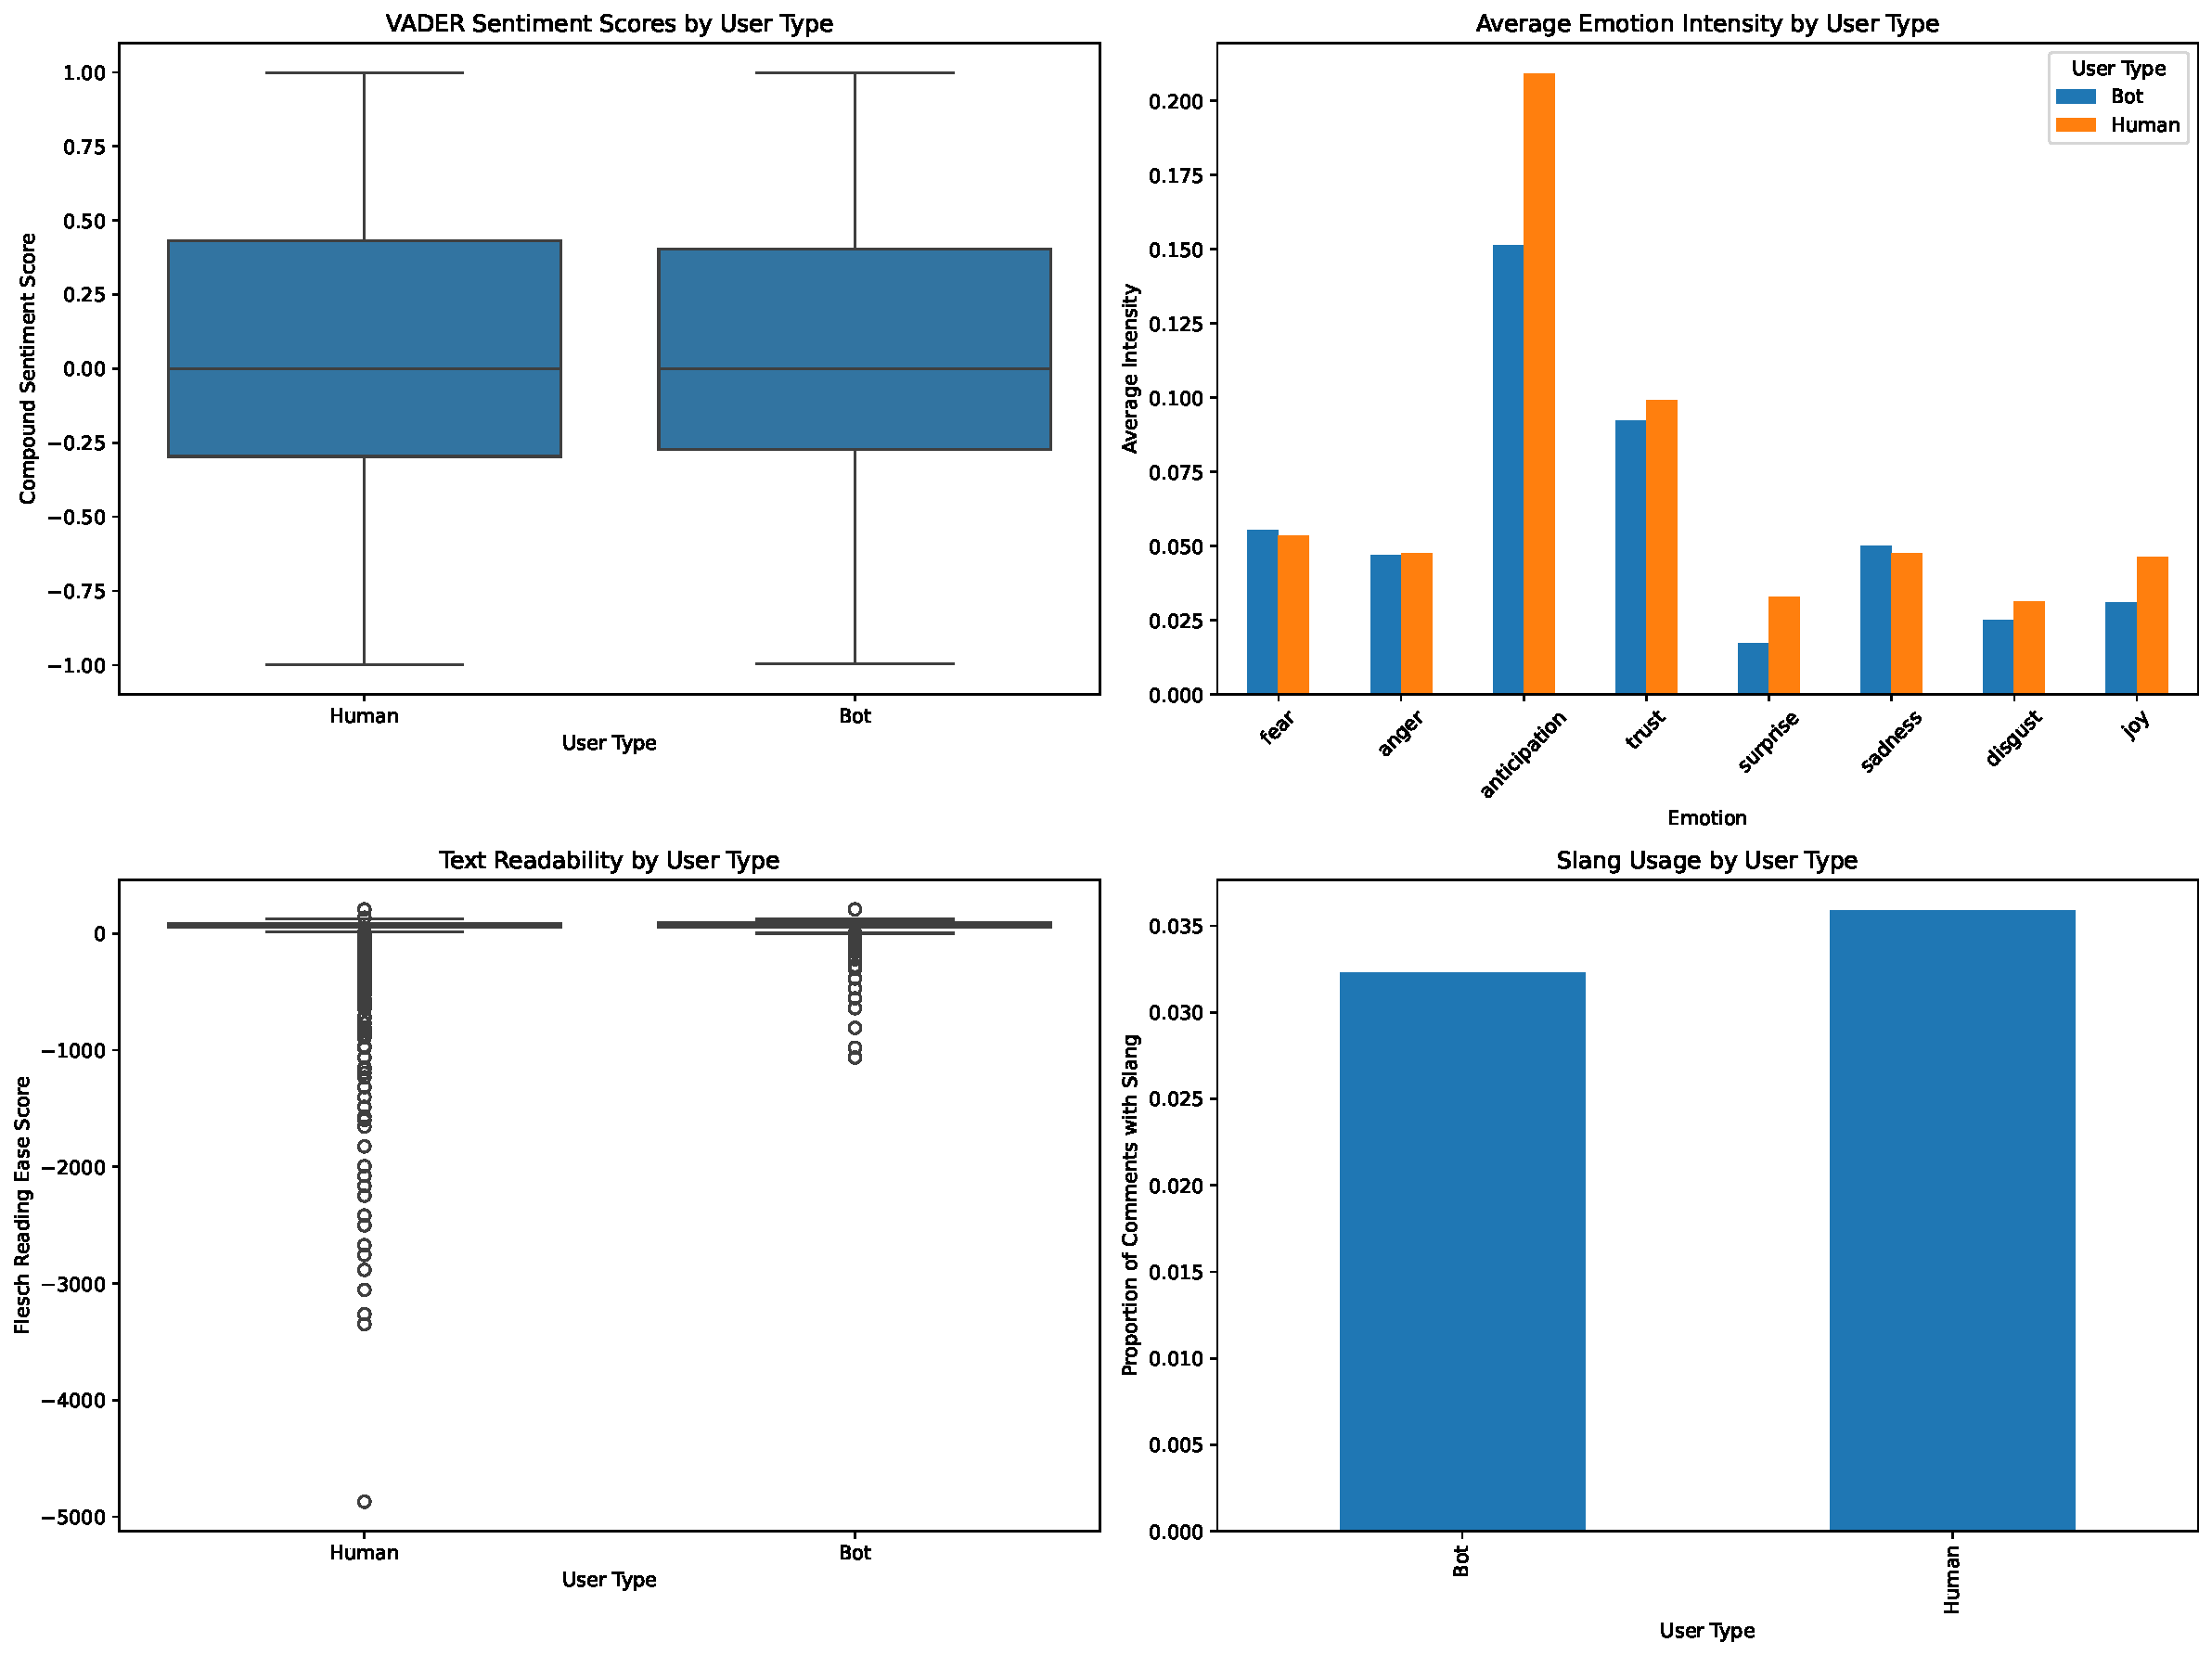
\includegraphics[keepaspectratio]{detecting_bots_on_reddit_code_files/figure-pdf/cell-26-output-1.pdf}}

\pandocbounded{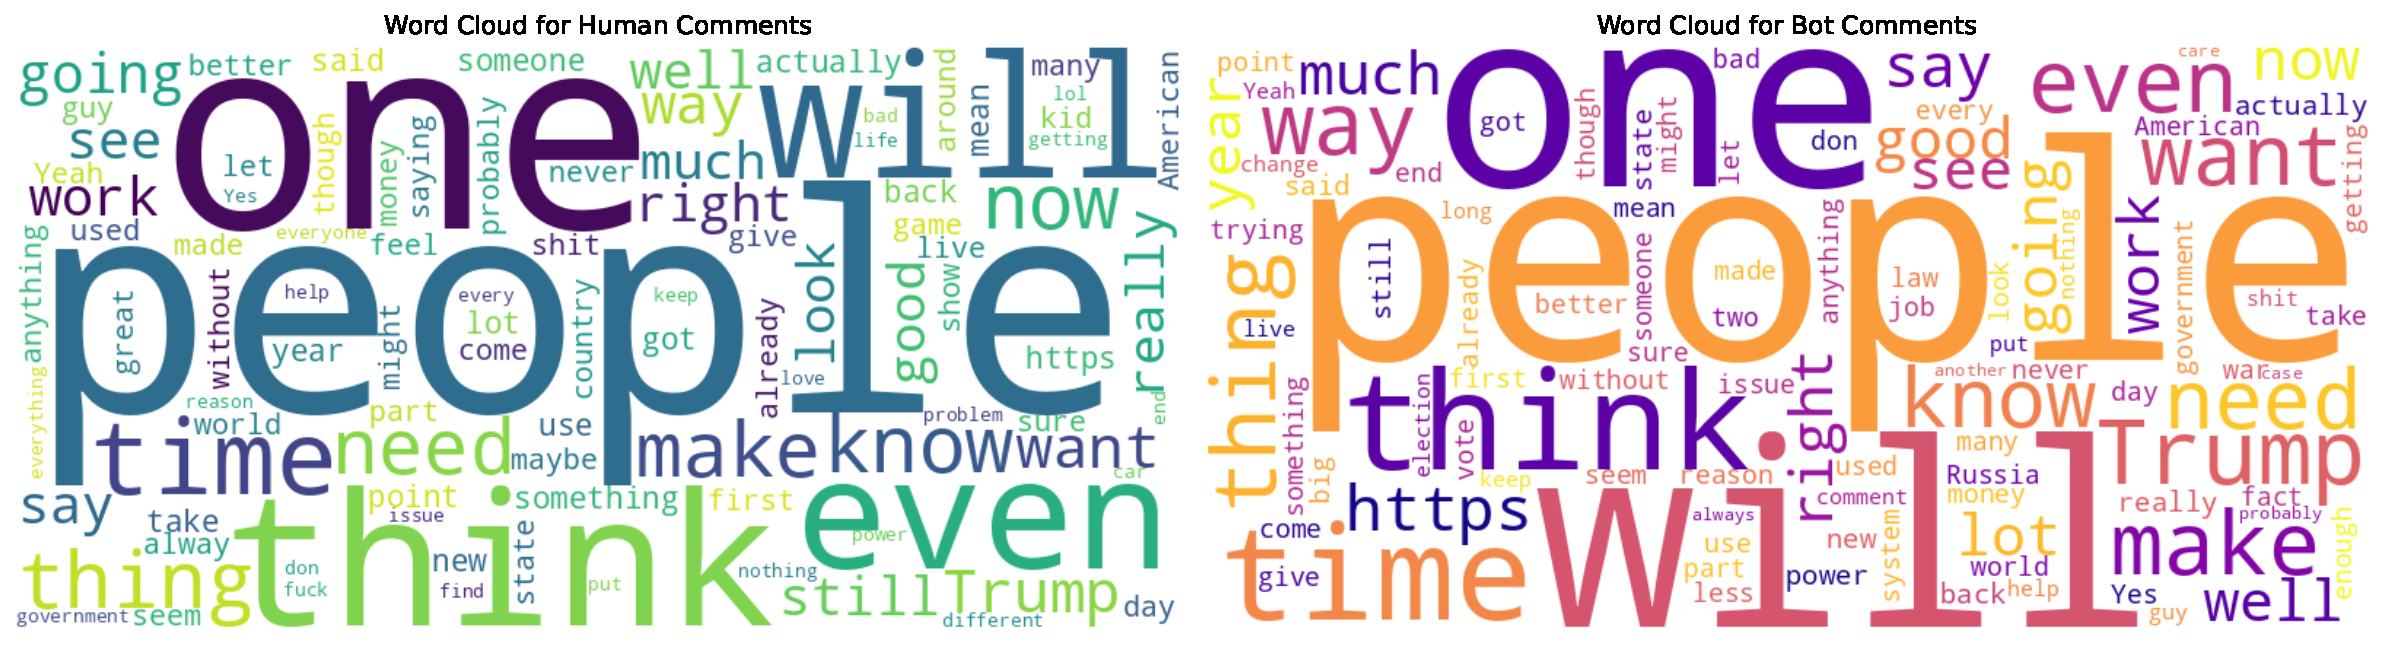
\includegraphics[keepaspectratio]{detecting_bots_on_reddit_code_files/figure-pdf/cell-26-output-2.pdf}}

\pandocbounded{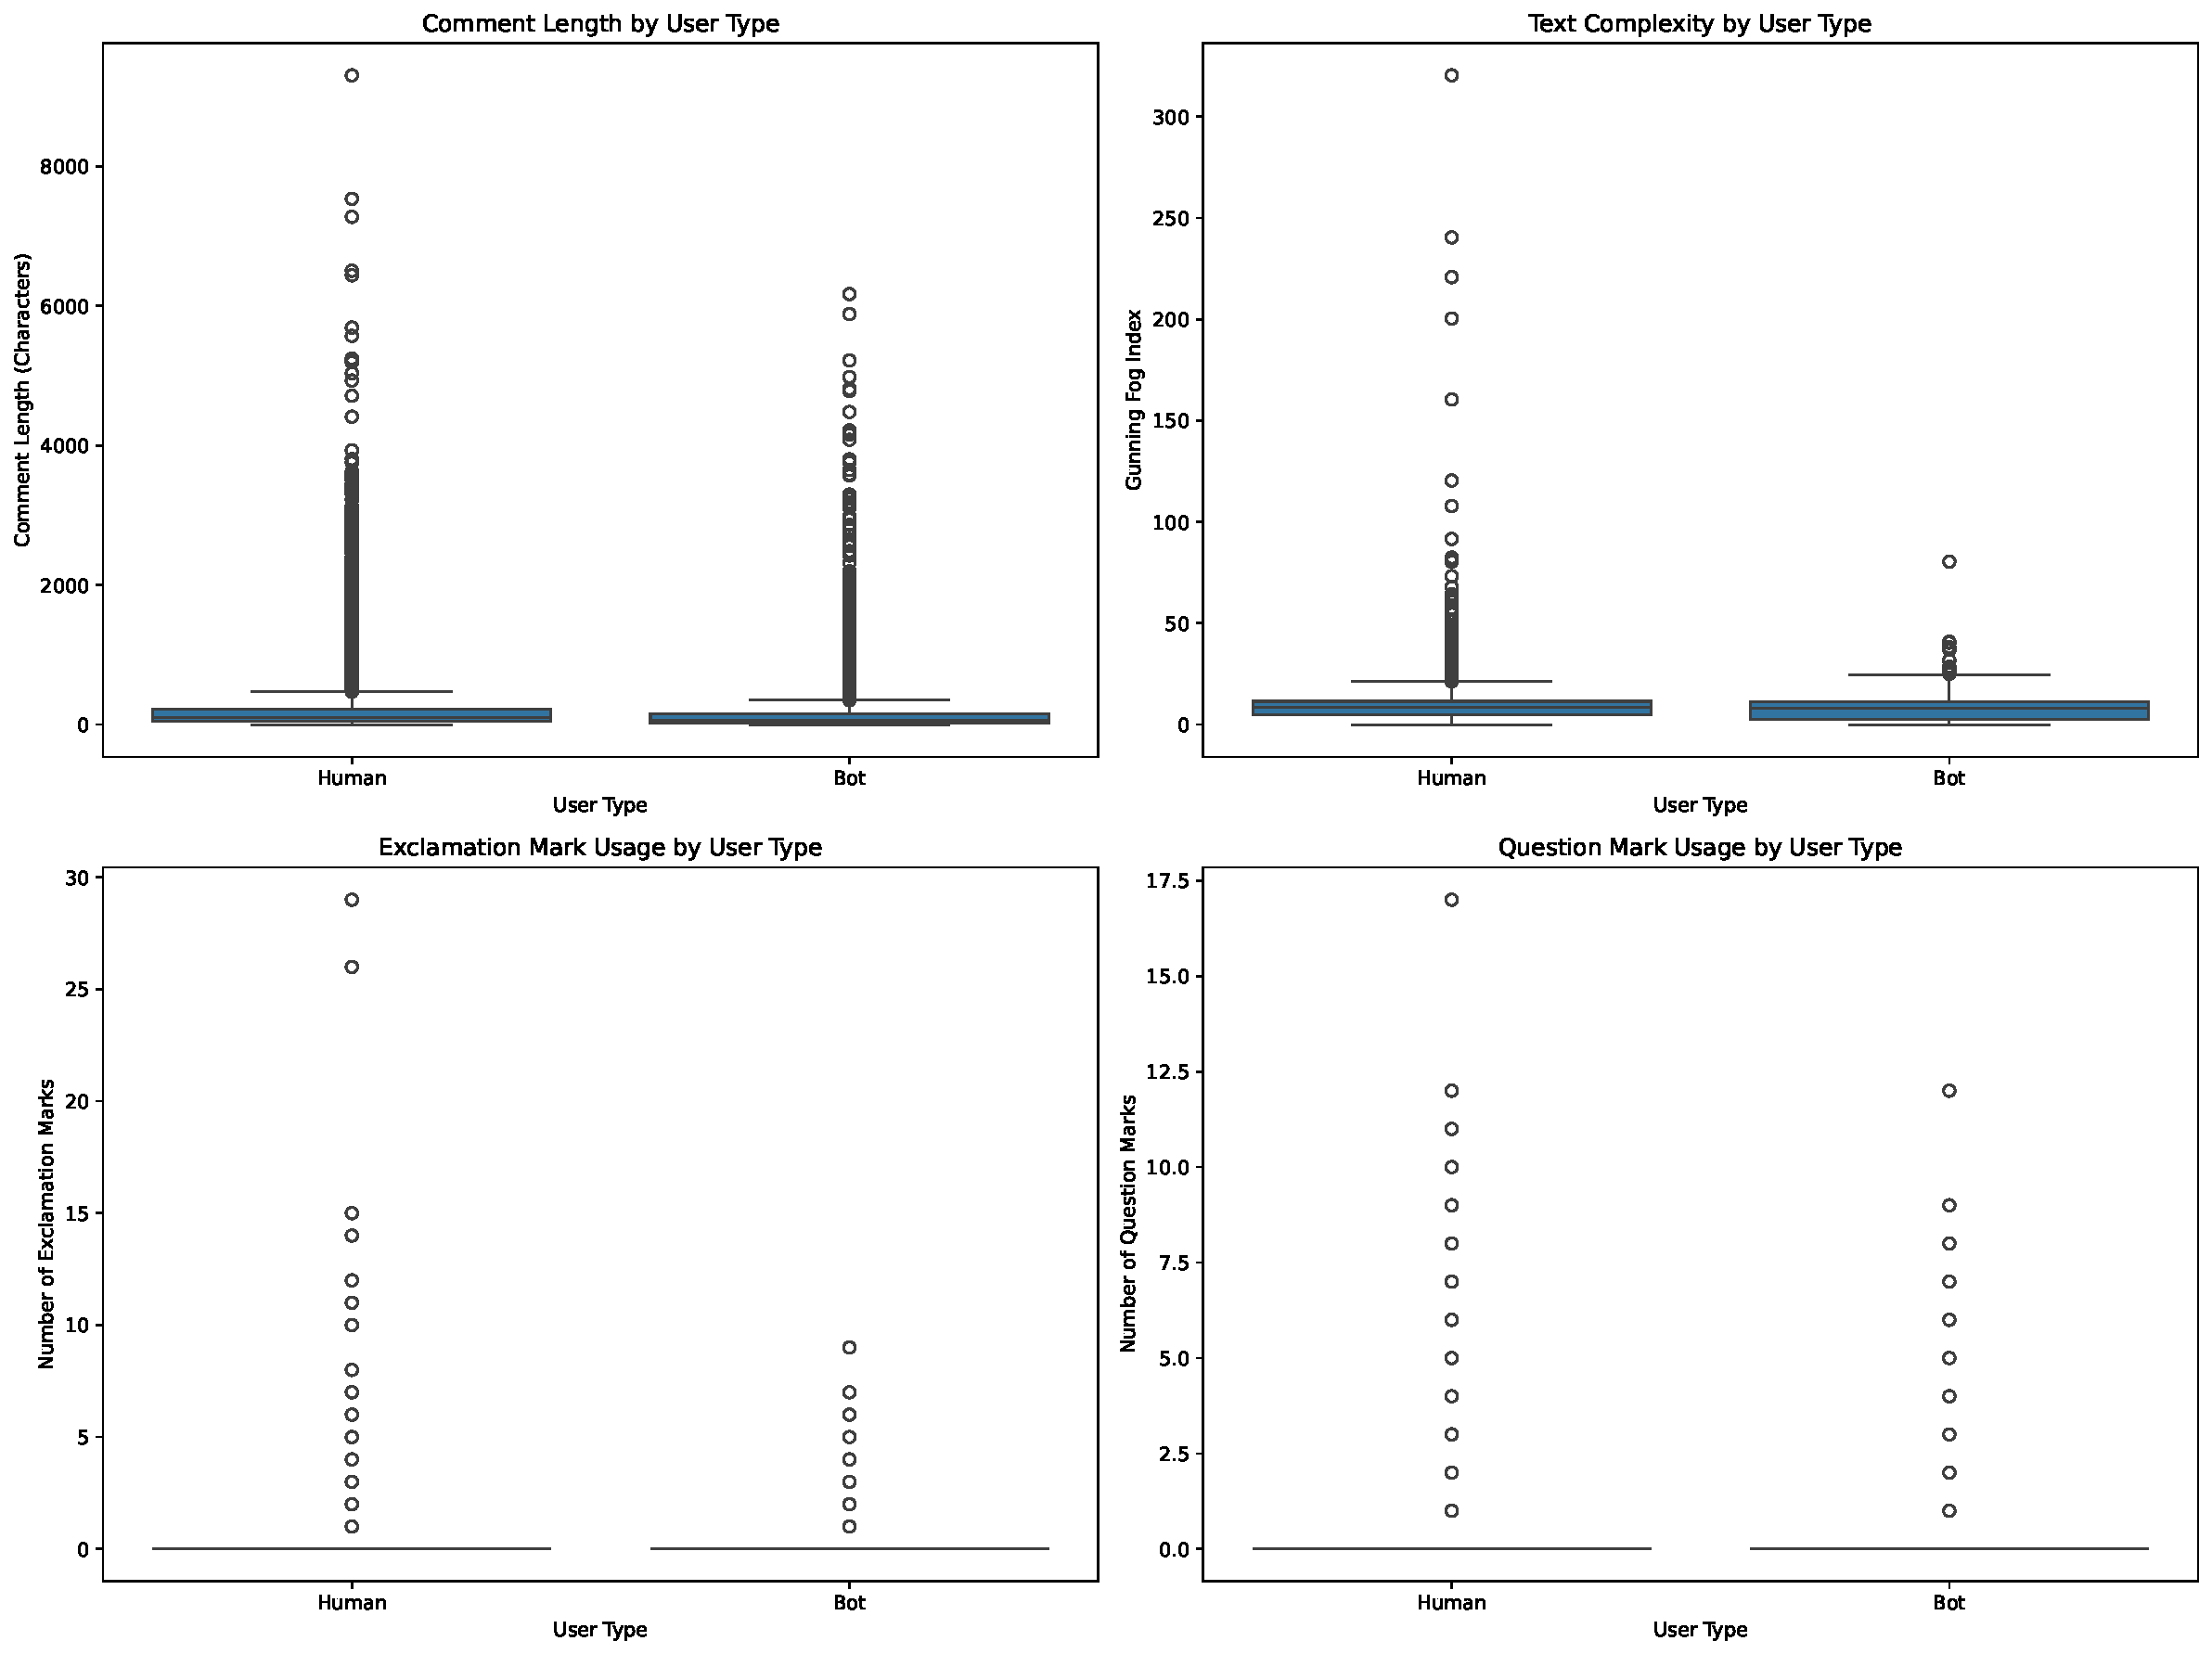
\includegraphics[keepaspectratio]{detecting_bots_on_reddit_code_files/figure-pdf/cell-26-output-3.pdf}}

\begin{verbatim}

=== SENTIMENT ANALYSIS SUMMARY ===

Human Average Sentiment: 0.0441
Bot Average Sentiment: 0.0419

Dominant Human Emotions:
- Anticipation: 0.2091
- Trust: 0.0991
- Fear: 0.0536

Dominant Bot Emotions:
- Anticipation: 0.1513
- Trust: 0.0924
- Fear: 0.0555

Top 10 Common Words in Human Comments:
- people: 8105
- time: 3823
- trump: 3117
- good: 3081
- really: 3058
- going: 2943
- want: 2852
- much: 2819
- way: 2809
- https: 2793

Top 10 Common Words in Bot Comments:
- people: 467
- trump: 204
- https: 188
- time: 185
- right: 162
- way: 161
- want: 146
- going: 144
- much: 144
- good: 138

Linguistic Style Comparison:
Human Average Readability Score: 64.40
Bot Average Readability Score: 67.72
Human Average Complexity Score: 8.89
Bot Average Complexity Score: 7.90
Human Slang Usage Rate: 3.59%
Bot Slang Usage Rate: 3.23%
\end{verbatim}

\begin{Shaded}
\begin{Highlighting}[]
\ImportTok{import}\NormalTok{ pandas }\ImportTok{as}\NormalTok{ pd}
\ImportTok{import}\NormalTok{ numpy }\ImportTok{as}\NormalTok{ np}
\ImportTok{import}\NormalTok{ seaborn }\ImportTok{as}\NormalTok{ sns}
\ImportTok{from}\NormalTok{ nltk.sentiment }\ImportTok{import}\NormalTok{ SentimentIntensityAnalyzer}
\ImportTok{from}\NormalTok{ textblob }\ImportTok{import}\NormalTok{ TextBlob}
\ImportTok{import}\NormalTok{ re}
\ImportTok{from}\NormalTok{ collections }\ImportTok{import}\NormalTok{ Counter}
\ImportTok{from}\NormalTok{ wordcloud }\ImportTok{import}\NormalTok{ WordCloud}
\ImportTok{import}\NormalTok{ nltk}
\ImportTok{from}\NormalTok{ nltk.tokenize }\ImportTok{import}\NormalTok{ word\_tokenize}
\ImportTok{from}\NormalTok{ nltk.corpus }\ImportTok{import}\NormalTok{ stopwords}
\ImportTok{import}\NormalTok{ string}
\ImportTok{from}\NormalTok{ sklearn.feature\_extraction.text }\ImportTok{import}\NormalTok{ CountVectorizer, TfidfVectorizer}
\ImportTok{import}\NormalTok{ textstat}
\ImportTok{from}\NormalTok{ nrclex }\ImportTok{import}\NormalTok{ NRCLex}

\CommentTok{\# Import necessary libraries}
\ImportTok{import}\NormalTok{ matplotlib.pyplot }\ImportTok{as}\NormalTok{ plt}

\CommentTok{\# Download necessary NLTK resources}
\NormalTok{nltk.download(}\StringTok{\textquotesingle{}punkt\textquotesingle{}}\NormalTok{, quiet}\OperatorTok{=}\VariableTok{True}\NormalTok{)}
\NormalTok{nltk.download(}\StringTok{\textquotesingle{}stopwords\textquotesingle{}}\NormalTok{, quiet}\OperatorTok{=}\VariableTok{True}\NormalTok{)}
\NormalTok{nltk.download(}\StringTok{\textquotesingle{}vader\_lexicon\textquotesingle{}}\NormalTok{, quiet}\OperatorTok{=}\VariableTok{True}\NormalTok{)}

\CommentTok{\# Sentiment Analysis by Subreddit}
\NormalTok{analyzer }\OperatorTok{=}\NormalTok{ SentimentIntensityAnalyzer()}
\NormalTok{processed\_comments[}\StringTok{\textquotesingle{}vader\_compound\textquotesingle{}}\NormalTok{] }\OperatorTok{=}\NormalTok{ processed\_comments[}\StringTok{\textquotesingle{}comment\_body\textquotesingle{}}\NormalTok{].}\BuiltInTok{apply}\NormalTok{(}\KeywordTok{lambda}\NormalTok{ x: analyzer.polarity\_scores(x)[}\StringTok{\textquotesingle{}compound\textquotesingle{}}\NormalTok{])}

\CommentTok{\# Group by subreddit and calculate average sentiment}
\NormalTok{subreddit\_sentiment }\OperatorTok{=}\NormalTok{ processed\_comments.groupby(}\StringTok{\textquotesingle{}subreddit\textquotesingle{}}\NormalTok{)[}\StringTok{\textquotesingle{}vader\_compound\textquotesingle{}}\NormalTok{].mean().sort\_values(ascending}\OperatorTok{=}\VariableTok{False}\NormalTok{)}

\CommentTok{\# Plotting the sentiment by subreddit}
\NormalTok{plt.figure(figsize}\OperatorTok{=}\NormalTok{(}\DecValTok{12}\NormalTok{, }\DecValTok{8}\NormalTok{))}
\NormalTok{subreddit\_sentiment.plot(kind}\OperatorTok{=}\StringTok{\textquotesingle{}bar\textquotesingle{}}\NormalTok{)}
\NormalTok{plt.title(}\StringTok{\textquotesingle{}Average Sentiment by Subreddit\textquotesingle{}}\NormalTok{)}
\NormalTok{plt.xlabel(}\StringTok{\textquotesingle{}Subreddit\textquotesingle{}}\NormalTok{)}
\NormalTok{plt.ylabel(}\StringTok{\textquotesingle{}Average Compound Sentiment Score\textquotesingle{}}\NormalTok{)}
\NormalTok{plt.xticks(rotation}\OperatorTok{=}\DecValTok{45}\NormalTok{, ha}\OperatorTok{=}\StringTok{\textquotesingle{}right\textquotesingle{}}\NormalTok{)}
\NormalTok{plt.tight\_layout()}
\NormalTok{plt.show()}

\CommentTok{\# Word Clouds by Subreddit}
\KeywordTok{def}\NormalTok{ generate\_word\_cloud(text, title):}
\NormalTok{    wordcloud }\OperatorTok{=}\NormalTok{ WordCloud(width}\OperatorTok{=}\DecValTok{800}\NormalTok{, height}\OperatorTok{=}\DecValTok{400}\NormalTok{, background\_color}\OperatorTok{=}\StringTok{\textquotesingle{}white\textquotesingle{}}\NormalTok{, min\_word\_length}\OperatorTok{=}\DecValTok{3}\NormalTok{).generate(text)}
\NormalTok{    plt.figure(figsize}\OperatorTok{=}\NormalTok{(}\DecValTok{10}\NormalTok{, }\DecValTok{5}\NormalTok{))}
\NormalTok{    plt.imshow(wordcloud, interpolation}\OperatorTok{=}\StringTok{\textquotesingle{}bilinear\textquotesingle{}}\NormalTok{)}
\NormalTok{    plt.title(title)}
\NormalTok{    plt.axis(}\StringTok{\textquotesingle{}off\textquotesingle{}}\NormalTok{)}
\NormalTok{    plt.show()}

\CommentTok{\# Group comments by subreddit}
\NormalTok{grouped\_comments }\OperatorTok{=}\NormalTok{ processed\_comments.groupby(}\StringTok{\textquotesingle{}subreddit\textquotesingle{}}\NormalTok{)[}\StringTok{\textquotesingle{}comment\_body\textquotesingle{}}\NormalTok{].}\BuiltInTok{apply}\NormalTok{(}\KeywordTok{lambda}\NormalTok{ x: }\StringTok{\textquotesingle{} \textquotesingle{}}\NormalTok{.join(x))}

\CommentTok{\# Generate word clouds for top subreddits}
\NormalTok{top\_n }\OperatorTok{=} \DecValTok{5}  \CommentTok{\# Number of top subreddits to display}
\NormalTok{top\_subreddits }\OperatorTok{=}\NormalTok{ grouped\_comments.head(top\_n)}

\ControlFlowTok{for}\NormalTok{ subreddit, text }\KeywordTok{in}\NormalTok{ top\_subreddits.items():}
\NormalTok{    generate\_word\_cloud(text, }\SpecialStringTok{f\textquotesingle{}Word Cloud for /r/}\SpecialCharTok{\{}\NormalTok{subreddit}\SpecialCharTok{\}}\SpecialStringTok{\textquotesingle{}}\NormalTok{)}
\end{Highlighting}
\end{Shaded}

\pandocbounded{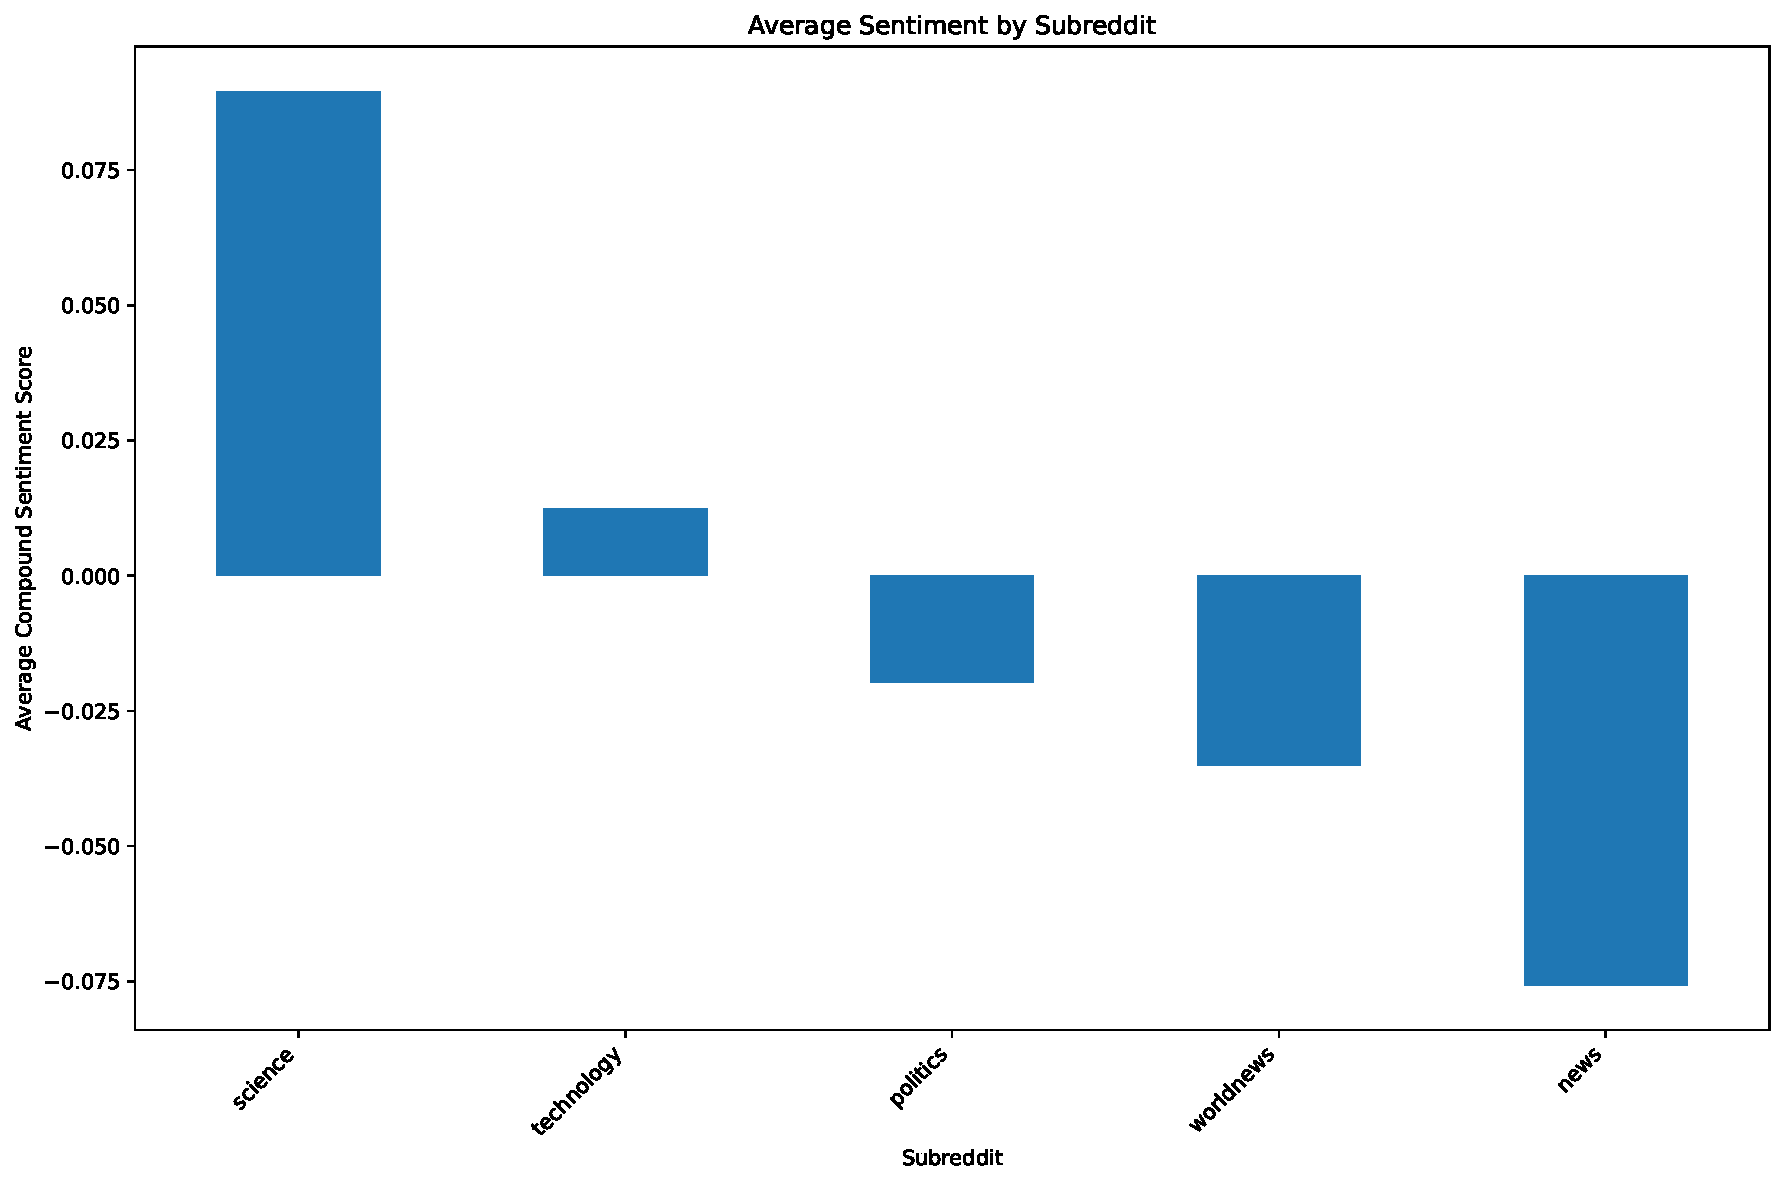
\includegraphics[keepaspectratio]{detecting_bots_on_reddit_code_files/figure-pdf/cell-27-output-1.pdf}}

\pandocbounded{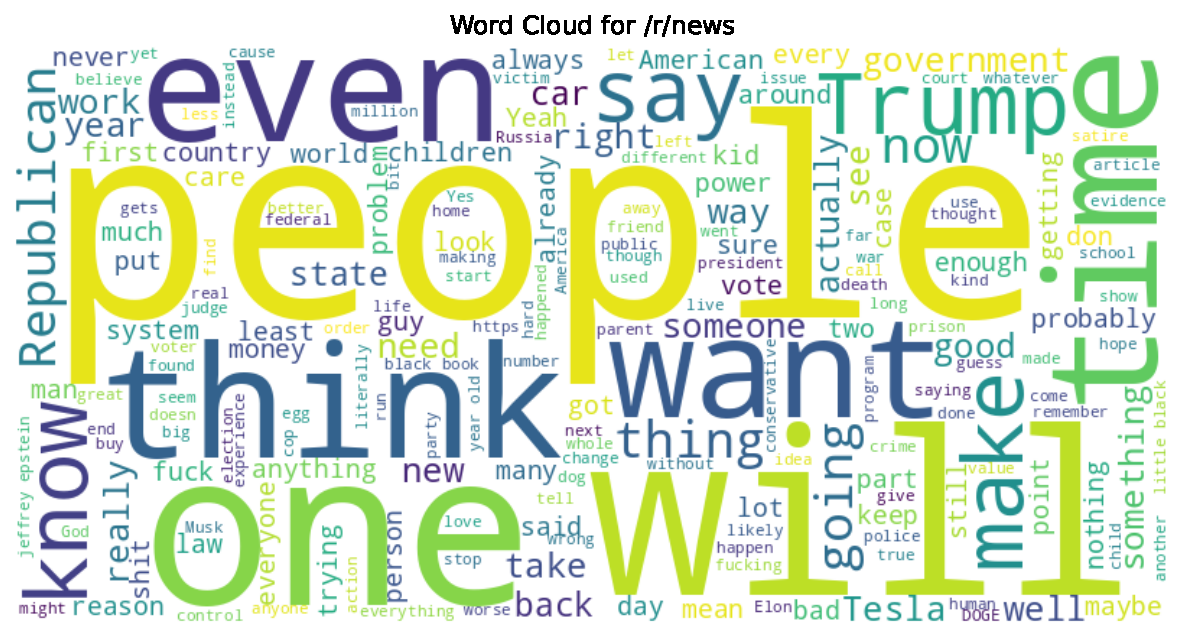
\includegraphics[keepaspectratio]{detecting_bots_on_reddit_code_files/figure-pdf/cell-27-output-2.pdf}}

\pandocbounded{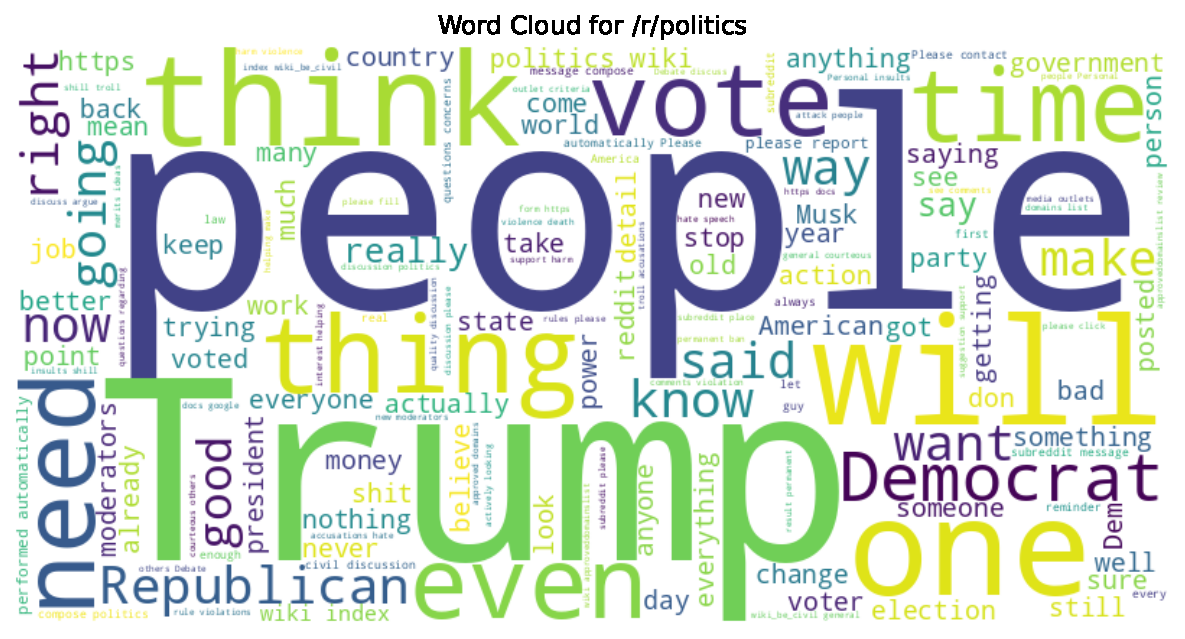
\includegraphics[keepaspectratio]{detecting_bots_on_reddit_code_files/figure-pdf/cell-27-output-3.pdf}}

\pandocbounded{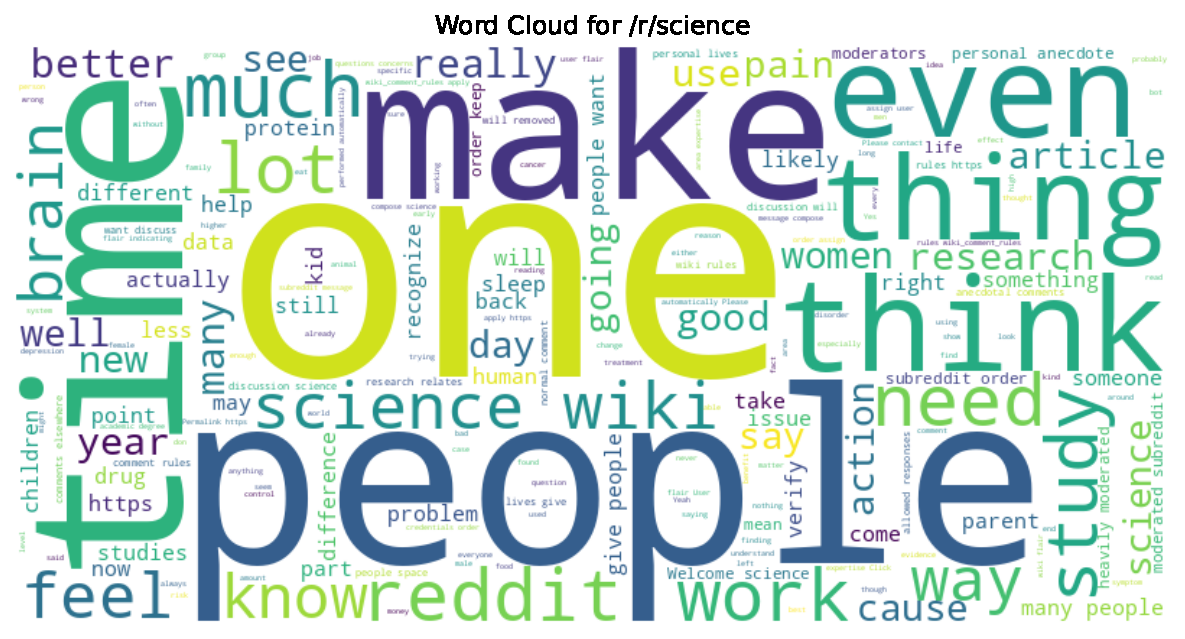
\includegraphics[keepaspectratio]{detecting_bots_on_reddit_code_files/figure-pdf/cell-27-output-4.pdf}}

\pandocbounded{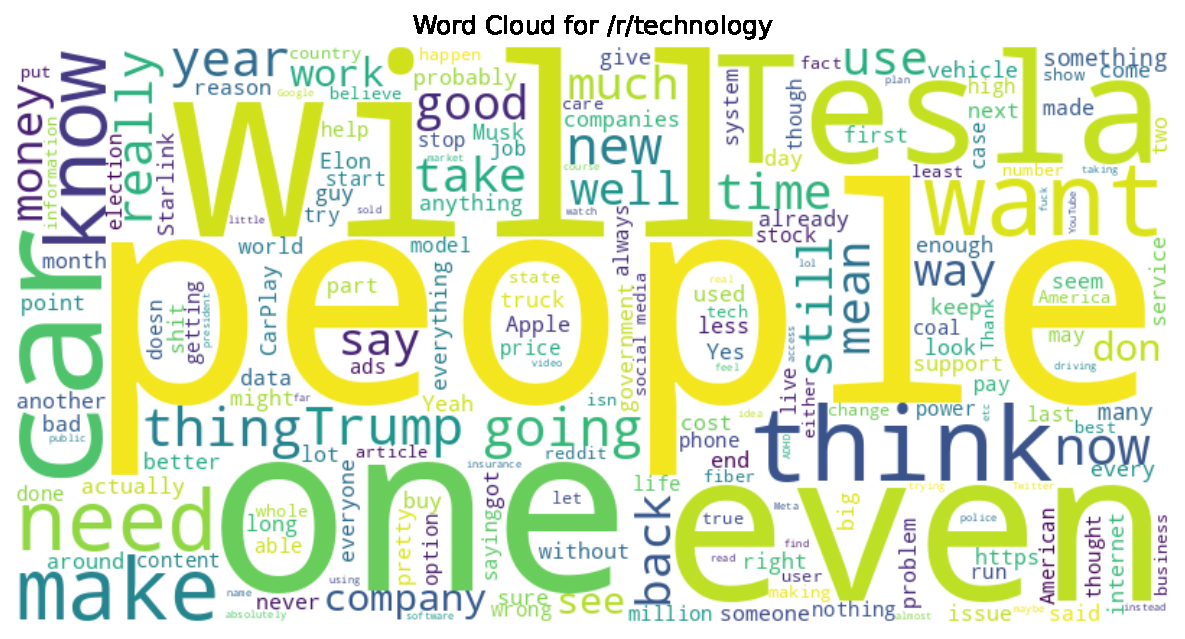
\includegraphics[keepaspectratio]{detecting_bots_on_reddit_code_files/figure-pdf/cell-27-output-5.pdf}}

\pandocbounded{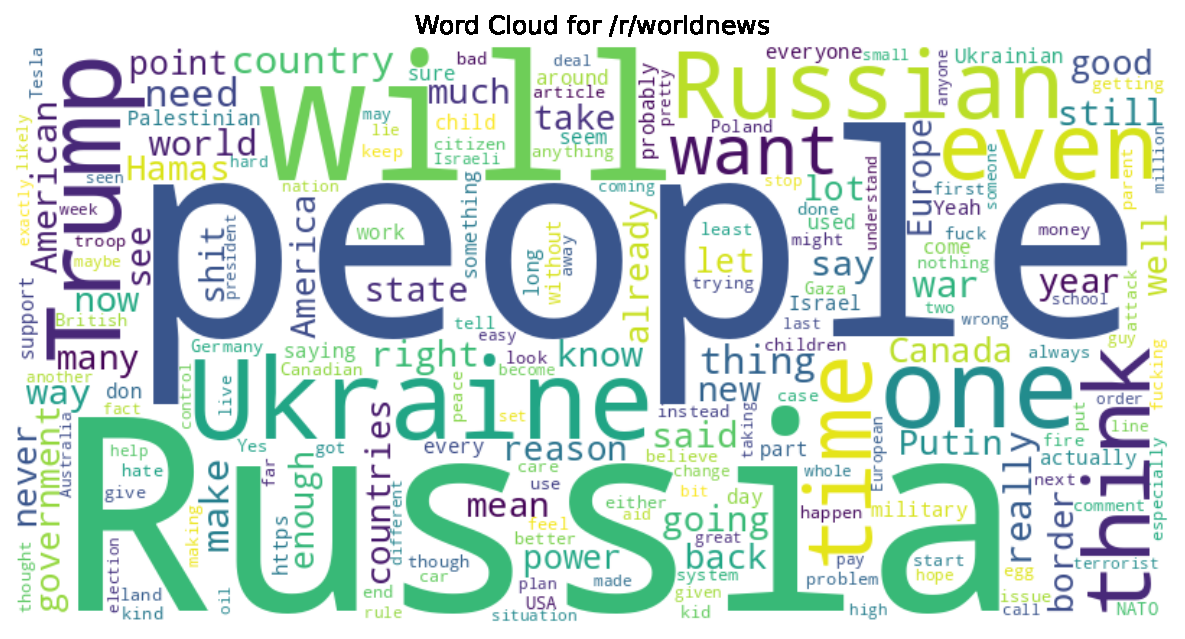
\includegraphics[keepaspectratio]{detecting_bots_on_reddit_code_files/figure-pdf/cell-27-output-6.pdf}}

\begin{Shaded}
\begin{Highlighting}[]
\ImportTok{from}\NormalTok{ sklearn.feature\_extraction.text }\ImportTok{import}\NormalTok{ TfidfVectorizer}
\ImportTok{from}\NormalTok{ sklearn.metrics.pairwise }\ImportTok{import}\NormalTok{ cosine\_similarity}
\ImportTok{import}\NormalTok{ seaborn }\ImportTok{as}\NormalTok{ sns}
\ImportTok{import}\NormalTok{ numpy }\ImportTok{as}\NormalTok{ np}

\CommentTok{\# Create subreddit cross{-}similarity heatmaps}
\ImportTok{import}\NormalTok{ matplotlib.pyplot }\ImportTok{as}\NormalTok{ plt}

\CommentTok{\# Group comments by subreddit}
\NormalTok{subreddit\_texts }\OperatorTok{=}\NormalTok{ processed\_comments.groupby(}\StringTok{\textquotesingle{}subreddit\textquotesingle{}}\NormalTok{)[}\StringTok{\textquotesingle{}comment\_body\textquotesingle{}}\NormalTok{].}\BuiltInTok{apply}\NormalTok{(}\KeywordTok{lambda}\NormalTok{ x: }\StringTok{\textquotesingle{} \textquotesingle{}}\NormalTok{.join(x))}

\CommentTok{\# Get the top subreddits by comment count}
\NormalTok{top\_subreddits }\OperatorTok{=}\NormalTok{ processed\_comments[}\StringTok{\textquotesingle{}subreddit\textquotesingle{}}\NormalTok{].value\_counts().head(}\DecValTok{15}\NormalTok{).index.tolist()}

\CommentTok{\# Filter to include only top subreddits}
\NormalTok{filtered\_texts }\OperatorTok{=}\NormalTok{ subreddit\_texts[subreddit\_texts.index.isin(top\_subreddits)]}

\CommentTok{\# Calculate TF{-}IDF vectors for each subreddit\textquotesingle{}s combined text}
\NormalTok{vectorizer }\OperatorTok{=}\NormalTok{ TfidfVectorizer(max\_features}\OperatorTok{=}\DecValTok{5000}\NormalTok{, stop\_words}\OperatorTok{=}\StringTok{\textquotesingle{}english\textquotesingle{}}\NormalTok{, min\_df}\OperatorTok{=}\DecValTok{2}\NormalTok{)}
\NormalTok{tfidf\_matrix }\OperatorTok{=}\NormalTok{ vectorizer.fit\_transform(filtered\_texts)}

\CommentTok{\# Calculate cosine similarity between subreddits}
\NormalTok{similarity\_matrix }\OperatorTok{=}\NormalTok{ cosine\_similarity(tfidf\_matrix)}

\CommentTok{\# Create a DataFrame for the similarity matrix}
\NormalTok{similarity\_df }\OperatorTok{=}\NormalTok{ pd.DataFrame(}
\NormalTok{    similarity\_matrix, }
\NormalTok{    index}\OperatorTok{=}\NormalTok{filtered\_texts.index, }
\NormalTok{    columns}\OperatorTok{=}\NormalTok{filtered\_texts.index}
\NormalTok{)}

\CommentTok{\# Plot the heatmap}
\NormalTok{plt.figure(figsize}\OperatorTok{=}\NormalTok{(}\DecValTok{12}\NormalTok{, }\DecValTok{10}\NormalTok{))}
\NormalTok{sns.heatmap(similarity\_df, annot}\OperatorTok{=}\VariableTok{True}\NormalTok{, cmap}\OperatorTok{=}\StringTok{\textquotesingle{}YlGnBu\textquotesingle{}}\NormalTok{, vmin}\OperatorTok{=}\FloatTok{0.5}\NormalTok{, vmax}\OperatorTok{=}\DecValTok{1}\NormalTok{, linewidths}\OperatorTok{=}\FloatTok{0.5}\NormalTok{)}
\NormalTok{plt.title(}\StringTok{\textquotesingle{}Cross{-}Subreddit Content Similarity Heatmap\textquotesingle{}}\NormalTok{)}
\NormalTok{plt.tight\_layout()}
\NormalTok{plt.show()}

\CommentTok{\# Extract the most distinguishing terms for each subreddit}
\NormalTok{feature\_names }\OperatorTok{=}\NormalTok{ np.array(vectorizer.get\_feature\_names\_out())}

\KeywordTok{def}\NormalTok{ get\_top\_features(tfidf\_matrix, feature\_names, top\_n}\OperatorTok{=}\DecValTok{10}\NormalTok{):}
    \CommentTok{"""Get the top N most distinctive features for each subreddit"""}
\NormalTok{    top\_features }\OperatorTok{=}\NormalTok{ \{\}}
    
    \ControlFlowTok{for}\NormalTok{ i, subreddit }\KeywordTok{in} \BuiltInTok{enumerate}\NormalTok{(filtered\_texts.index):}
        \CommentTok{\# Get the TF{-}IDF scores for this subreddit}
\NormalTok{        tfidf\_scores }\OperatorTok{=}\NormalTok{ tfidf\_matrix[i].toarray().flatten()}
        
        \CommentTok{\# Get indices of top N features}
\NormalTok{        top\_indices }\OperatorTok{=}\NormalTok{ tfidf\_scores.argsort()[}\OperatorTok{{-}}\NormalTok{top\_n:][::}\OperatorTok{{-}}\DecValTok{1}\NormalTok{]}
        
        \CommentTok{\# Get feature names and scores}
\NormalTok{        top\_terms }\OperatorTok{=}\NormalTok{ [(feature\_names[idx], tfidf\_scores[idx]) }\ControlFlowTok{for}\NormalTok{ idx }\KeywordTok{in}\NormalTok{ top\_indices]}
        
\NormalTok{        top\_features[subreddit] }\OperatorTok{=}\NormalTok{ top\_terms}
    
    \ControlFlowTok{return}\NormalTok{ top\_features}

\NormalTok{subreddit\_top\_terms }\OperatorTok{=}\NormalTok{ get\_top\_features(tfidf\_matrix, feature\_names)}
\end{Highlighting}
\end{Shaded}

\pandocbounded{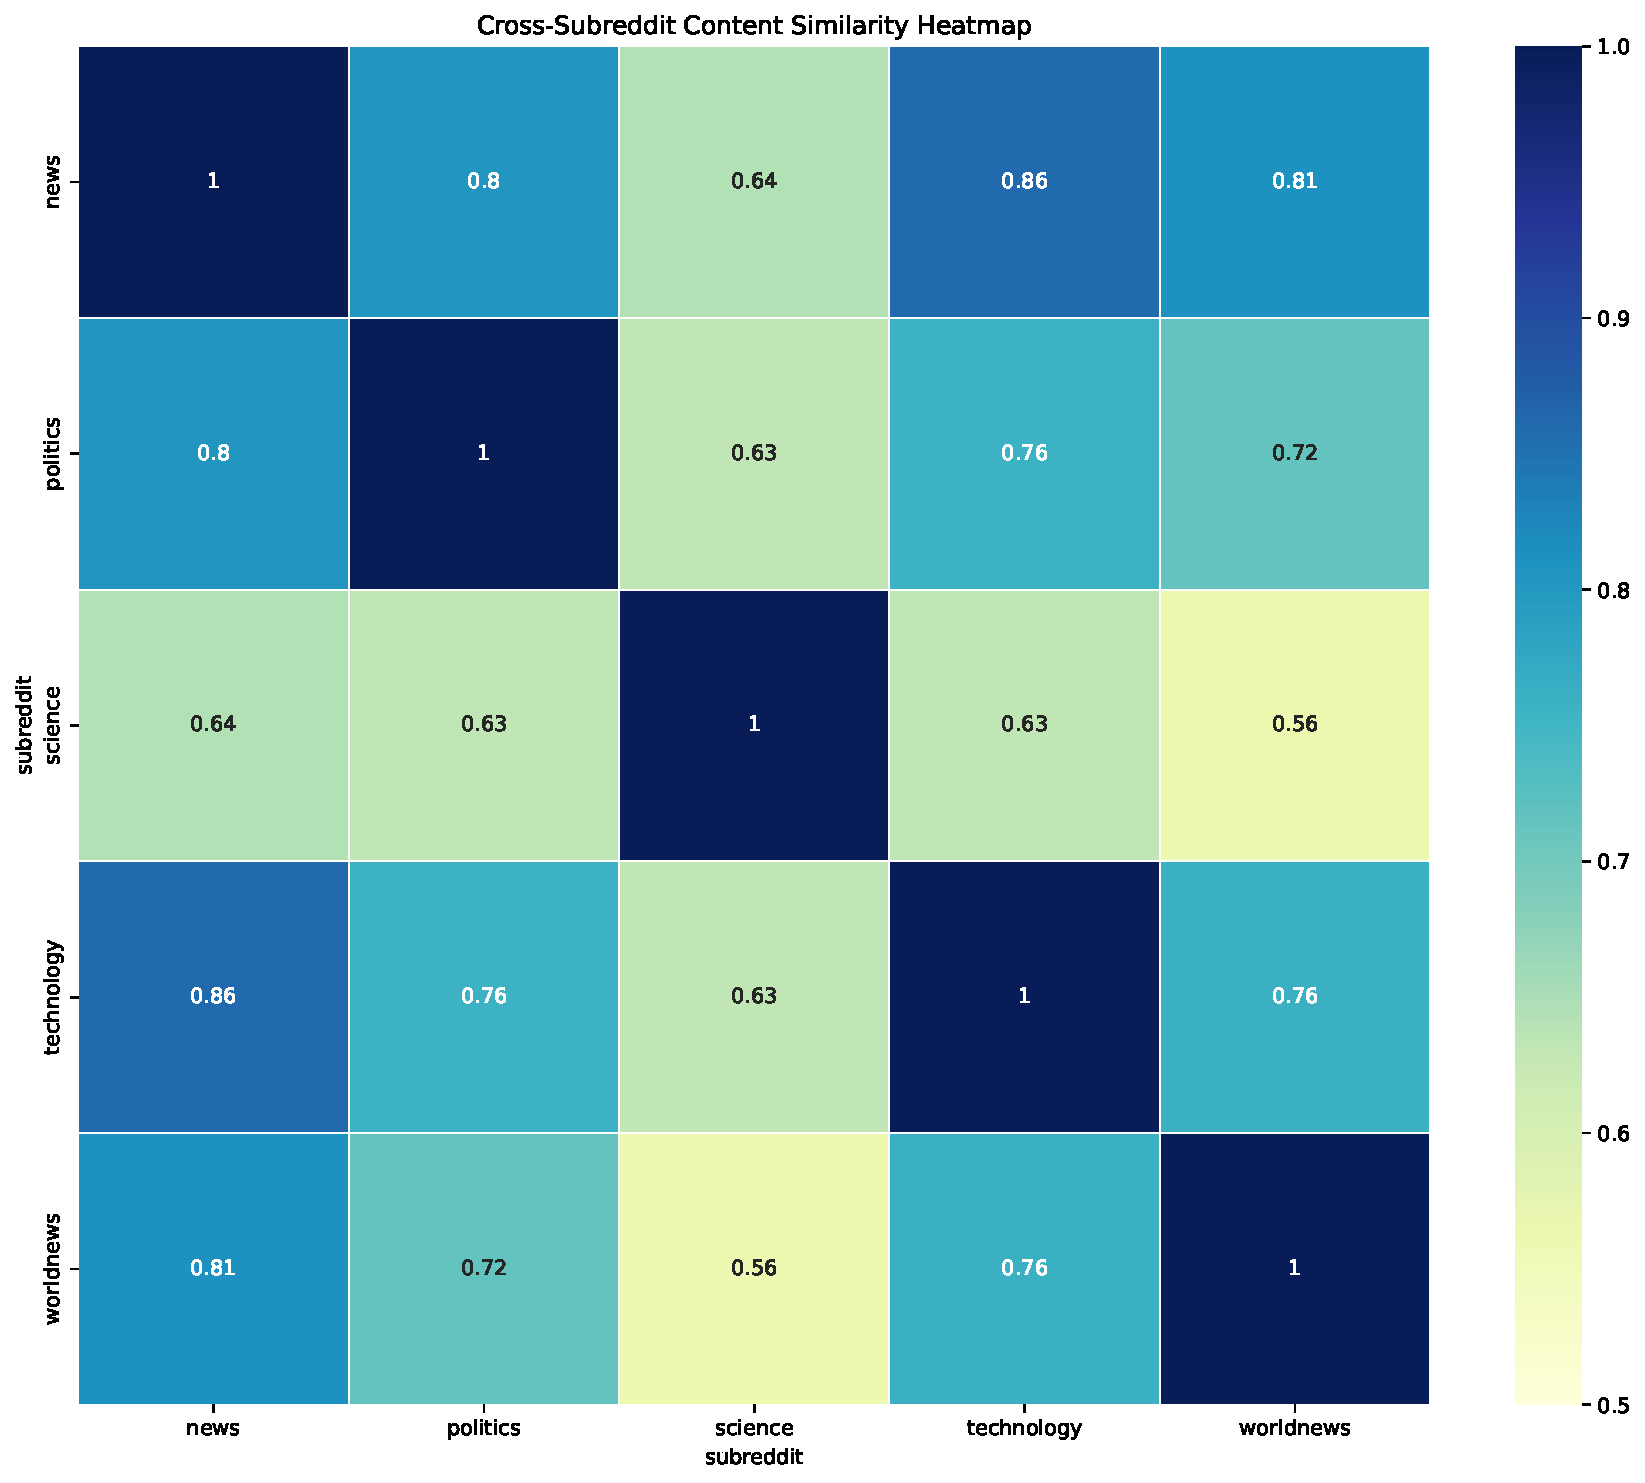
\includegraphics[keepaspectratio]{detecting_bots_on_reddit_code_files/figure-pdf/cell-28-output-1.pdf}}

\begin{Shaded}
\begin{Highlighting}[]
\ImportTok{import}\NormalTok{ os}
\ImportTok{import}\NormalTok{ pandas }\ImportTok{as}\NormalTok{ pd}
\ImportTok{import}\NormalTok{ matplotlib.pyplot }\ImportTok{as}\NormalTok{ plt}
\ImportTok{from}\NormalTok{ google }\ImportTok{import}\NormalTok{ genai}
\ImportTok{from}\NormalTok{ google.genai }\ImportTok{import}\NormalTok{ types}
\ImportTok{from}\NormalTok{ wordcloud }\ImportTok{import}\NormalTok{ WordCloud}
\ImportTok{import}\NormalTok{ random}

\CommentTok{\# {-}{-}{-}{-}{-} Step 1: Extract Top 5 Subreddits from ml\_features {-}{-}{-}{-}{-}}
\CommentTok{\# Assume ml\_features is already in your environment.}
\NormalTok{top\_subreddits }\OperatorTok{=}\NormalTok{ ml\_features[}\StringTok{\textquotesingle{}subreddit\textquotesingle{}}\NormalTok{].value\_counts().head(}\DecValTok{5}\NormalTok{).index.tolist()}

\CommentTok{\# {-}{-}{-}{-}{-} Step 2: Stratified Sampling {-}{-}{-}{-}{-} }
\NormalTok{sampled\_comments }\OperatorTok{=}\NormalTok{ \{\}}
\NormalTok{sample\_size }\OperatorTok{=} \DecValTok{100}
\ControlFlowTok{for}\NormalTok{ subreddit }\KeywordTok{in}\NormalTok{ top\_subreddits:}
\NormalTok{    subreddit\_comments }\OperatorTok{=}\NormalTok{ ml\_features[ml\_features[}\StringTok{\textquotesingle{}subreddit\textquotesingle{}}\NormalTok{] }\OperatorTok{==}\NormalTok{ subreddit][}\StringTok{\textquotesingle{}comment\_body\textquotesingle{}}\NormalTok{]}
    \ControlFlowTok{if} \BuiltInTok{len}\NormalTok{(subreddit\_comments) }\OperatorTok{\textgreater{}}\NormalTok{ sample\_size:}
\NormalTok{        sampled }\OperatorTok{=}\NormalTok{ subreddit\_comments.sample(n}\OperatorTok{=}\NormalTok{sample\_size, random\_state}\OperatorTok{=}\DecValTok{42}\NormalTok{)}
    \ControlFlowTok{else}\NormalTok{:}
\NormalTok{        sampled }\OperatorTok{=}\NormalTok{ subreddit\_comments}
\NormalTok{    sampled\_comments[subreddit] }\OperatorTok{=}\NormalTok{ sampled.tolist()}

\CommentTok{\# {-}{-}{-}{-}{-} Step 3: Gemini API generate() Function {-}{-}{-}{-}{-}}
\KeywordTok{def}\NormalTok{ generate(prompt):}
\NormalTok{    client }\OperatorTok{=}\NormalTok{ genai.Client(}
\NormalTok{        api\_key}\OperatorTok{=}\NormalTok{os.getenv(}\StringTok{"GEMINI\_API\_KEY"}\NormalTok{),}
\NormalTok{    )}
\NormalTok{    model }\OperatorTok{=} \StringTok{"gemini{-}2.0{-}flash"}
\NormalTok{    contents }\OperatorTok{=}\NormalTok{ [}
\NormalTok{        types.Content(}
\NormalTok{            role}\OperatorTok{=}\StringTok{"user"}\NormalTok{,}
\NormalTok{            parts}\OperatorTok{=}\NormalTok{[}
\NormalTok{                types.Part.from\_text(text}\OperatorTok{=}\NormalTok{prompt),}
\NormalTok{            ],}
\NormalTok{        ),}
\NormalTok{    ]}
\NormalTok{    generate\_content\_config }\OperatorTok{=}\NormalTok{ types.GenerateContentConfig(}
\NormalTok{        temperature}\OperatorTok{=}\DecValTok{0}\NormalTok{,}
\NormalTok{        top\_p}\OperatorTok{=}\DecValTok{0}\NormalTok{,}
\NormalTok{        top\_k}\OperatorTok{=}\DecValTok{1}\NormalTok{,}
\NormalTok{        max\_output\_tokens}\OperatorTok{=}\DecValTok{8192}\NormalTok{,}
\NormalTok{        response\_mime\_type}\OperatorTok{=}\StringTok{"text/plain"}\NormalTok{,}
\NormalTok{    )}
\NormalTok{    complete\_response }\OperatorTok{=} \StringTok{""}
    \ControlFlowTok{for}\NormalTok{ chunk }\KeywordTok{in}\NormalTok{ client.models.generate\_content\_stream(}
\NormalTok{        model}\OperatorTok{=}\NormalTok{model,}
\NormalTok{        contents}\OperatorTok{=}\NormalTok{contents,}
\NormalTok{        config}\OperatorTok{=}\NormalTok{generate\_content\_config,}
\NormalTok{    ):}
\NormalTok{        complete\_response }\OperatorTok{+=}\NormalTok{ chunk.text}
    \ControlFlowTok{return}\NormalTok{ complete\_response.strip()}

\CommentTok{\# {-}{-}{-}{-}{-} Step 4: Query the LLM for Each Subreddit {-}{-}{-}{-}{-}}
\NormalTok{subreddit\_responses }\OperatorTok{=}\NormalTok{ \{\}}
\ControlFlowTok{for}\NormalTok{ subreddit, comments }\KeywordTok{in}\NormalTok{ sampled\_comments.items():}
    \CommentTok{\# Take a random sample of comments if there are too many}
    \ControlFlowTok{if} \BuiltInTok{len}\NormalTok{(}\StringTok{" "}\NormalTok{.join(comments)) }\OperatorTok{\textgreater{}} \DecValTok{4000}\NormalTok{:}
\NormalTok{        random.seed(}\DecValTok{42}\NormalTok{)  }\CommentTok{\# For reproducibility}
\NormalTok{        sampled\_comments }\OperatorTok{=}\NormalTok{ random.sample(comments, }\BuiltInTok{min}\NormalTok{(}\BuiltInTok{len}\NormalTok{(comments), }\DecValTok{50}\NormalTok{))}
\NormalTok{        text\_blob }\OperatorTok{=} \StringTok{" "}\NormalTok{.join(sampled\_comments)[:}\DecValTok{4000}\NormalTok{]}
    \ControlFlowTok{else}\NormalTok{:}
\NormalTok{        text\_blob }\OperatorTok{=} \StringTok{" "}\NormalTok{.join(comments)[:}\DecValTok{4000}\NormalTok{]}
\NormalTok{    prompt }\OperatorTok{=}\NormalTok{ (}
        \SpecialStringTok{f"Perform sentiment analysis on the following comments from subreddit /r/}\SpecialCharTok{\{}\NormalTok{subreddit}\SpecialCharTok{\}}\SpecialStringTok{. "}
        \StringTok{"Identify 20 unique keywords (based exclusively on the text you are fed) that capture the essence of this subreddit (which can later be used for word clouds), and provide a brief sentiment summary (e.g. note if the overall tone is positive, negative, or neutral). "}
        \StringTok{"At the end, on a new separate line, output exactly: \textquotesingle{}Keywords: keyword1, keyword2, etc.\textquotesingle{} followed by a comma{-}separated list of the keywords, with no extra text.}\CharTok{\textbackslash{}n\textbackslash{}n}\StringTok{Comments:}\CharTok{\textbackslash{}n}\StringTok{"} 
        \OperatorTok{+}\NormalTok{ text\_blob}
\NormalTok{    )}
\NormalTok{    response }\OperatorTok{=}\NormalTok{ generate(prompt)}
\NormalTok{    subreddit\_responses[subreddit] }\OperatorTok{=}\NormalTok{ response}
    \BuiltInTok{print}\NormalTok{(}\SpecialStringTok{f"/r/}\SpecialCharTok{\{}\NormalTok{subreddit}\SpecialCharTok{\}}\SpecialStringTok{ Response:}\CharTok{\textbackslash{}n}\SpecialCharTok{\{}\NormalTok{response}\SpecialCharTok{\}}\CharTok{\textbackslash{}n}\SpecialCharTok{\{}\StringTok{\textquotesingle{}{-}\textquotesingle{}}\OperatorTok{*}\DecValTok{60}\SpecialCharTok{\}}\CharTok{\textbackslash{}n}\SpecialStringTok{"}\NormalTok{)}

\CommentTok{\# {-}{-}{-}{-}{-} Step 5: Extract Keywords and Build Word Clouds {-}{-}{-}{-}{-}}
\ControlFlowTok{for}\NormalTok{ subreddit, response }\KeywordTok{in}\NormalTok{ subreddit\_responses.items():}
\NormalTok{    keywords\_line }\OperatorTok{=} \VariableTok{None}
    \ControlFlowTok{for}\NormalTok{ line }\KeywordTok{in}\NormalTok{ response.splitlines():}
        \ControlFlowTok{if}\NormalTok{ line.strip().startswith(}\StringTok{"Keywords:"}\NormalTok{):}
\NormalTok{            keywords\_line }\OperatorTok{=}\NormalTok{ line.strip()}
            \ControlFlowTok{break}
    \ControlFlowTok{if}\NormalTok{ keywords\_line:}
        \CommentTok{\# Remove the "Keywords:" prefix and extra spaces, then split by commas.}
\NormalTok{        keywords\_part }\OperatorTok{=}\NormalTok{ keywords\_line[}\BuiltInTok{len}\NormalTok{(}\StringTok{"Keywords:"}\NormalTok{):].strip()}
\NormalTok{        keywords }\OperatorTok{=}\NormalTok{ [kw.strip() }\ControlFlowTok{for}\NormalTok{ kw }\KeywordTok{in}\NormalTok{ keywords\_part.split(}\StringTok{","}\NormalTok{) }\ControlFlowTok{if}\NormalTok{ kw.strip()]}
    \ControlFlowTok{else}\NormalTok{:}
\NormalTok{        keywords }\OperatorTok{=}\NormalTok{ []}
    
    \ControlFlowTok{if}\NormalTok{ keywords:}
        \CommentTok{\# Create a text blob from keywords for word cloud generation.}
\NormalTok{        wordcloud\_text }\OperatorTok{=} \StringTok{" "}\NormalTok{.join(keywords)}
\NormalTok{        wc }\OperatorTok{=}\NormalTok{ WordCloud(width}\OperatorTok{=}\DecValTok{800}\NormalTok{, height}\OperatorTok{=}\DecValTok{400}\NormalTok{, background\_color}\OperatorTok{=}\StringTok{\textquotesingle{}white\textquotesingle{}}\NormalTok{, min\_word\_length}\OperatorTok{=}\DecValTok{3}\NormalTok{).generate(wordcloud\_text)}
\NormalTok{        plt.figure(figsize}\OperatorTok{=}\NormalTok{(}\DecValTok{8}\NormalTok{, }\DecValTok{4}\NormalTok{))}
\NormalTok{        plt.imshow(wc, interpolation}\OperatorTok{=}\StringTok{"bilinear"}\NormalTok{)}
\NormalTok{        plt.axis(}\StringTok{"off"}\NormalTok{)}
\NormalTok{        plt.title(}\SpecialStringTok{f"/r/}\SpecialCharTok{\{}\NormalTok{subreddit}\SpecialCharTok{\}}\SpecialStringTok{ Word Cloud"}\NormalTok{)}
\NormalTok{        plt.show()}
    \ControlFlowTok{else}\NormalTok{:}
        \BuiltInTok{print}\NormalTok{(}\SpecialStringTok{f"No valid keywords extracted for /r/}\SpecialCharTok{\{}\NormalTok{subreddit}\SpecialCharTok{\}}\SpecialStringTok{."}\NormalTok{)}
\end{Highlighting}
\end{Shaded}

\begin{verbatim}
/r/politics Response:
The overall sentiment is largely negative, with expressions of frustration, concern about political polarization, and criticism of both Republicans and Democrats. There's also a sense of urgency and a call for action.

Keywords: Trump, Democrats, voting, propaganda, lies, republicans, January 6th, election, voters, government, political, school, history, courts, conspiracy, senate, house, action, leaders, movement

Keywords: Trump, Democrats, voting, propaganda, lies, republicans, January 6th, election, voters, government, political, school, history, courts, conspiracy, senate, house, action, leaders, movement
------------------------------------------------------------

/r/worldnews Response:
The overall sentiment is largely negative, with concerns about international relations, political issues, economic downturns, and war. There are also some positive comments about nature and personal experiences in certain countries.

Keywords: US, Canada, Europe, war, Russia, Ukraine, business, tourism, refugees, immigrants, oil, gas, production, recession, Hamas, Palestine, aid, negligence, sabotage, Tesla

Keywords: US, Canada, Europe, war, Russia, Ukraine, business, tourism, refugees, immigrants, oil, gas, production, recession, Hamas, Palestine, aid, negligence, sabotage, Tesla
------------------------------------------------------------

/r/news Response:
The overall sentiment is largely negative, expressing frustration, anger, and distrust towards government agencies, political figures, and certain societal behaviors. There's also a sense of cynicism and disillusionment.

Keywords: deported, citizens, ICE, Trump, unvaccinated, hypocrisy, Democrats, American, people, government, AI, schools, healthcare, Iran, Iraq, terrorists, President, irresponsible, illegal, expulsion

Keywords: deported, citizens, ICE, Trump, unvaccinated, hypocrisy, Democrats, American, people, government, AI, schools, healthcare, Iran, Iraq, terrorists, President, irresponsible, illegal, expulsion
------------------------------------------------------------

/r/technology Response:
The overall sentiment is largely negative, expressing frustration with technology (ads, electric vehicles, social media), political concerns (US influence, trade wars), and societal issues (racism). There's also a sense of skepticism and distrust towards large corporations and government actions.

Keywords: ads, nuclear, electric vehicles, facebook, software, tesla, youtube, firefox, energy, climate change, silicon valley, trade war, US, browser, ad blocker, DEI, racism, trump, renewable, recall

Keywords: ads, nuclear, electric vehicles, facebook, software, tesla, youtube, firefox, energy, climate change, silicon valley, trade war, US, browser, ad blocker, DEI, racism, trump, renewable, recall
------------------------------------------------------------

/r/science Response:
Sentiment Summary: The overall tone is mixed, with elements of curiosity, skepticism, personal anecdotes, and concern, particularly regarding mental health and the impact of the COVID-19 pandemic. There's also a critical perspective on the influence of funding and societal structures on scientific research.

Keywords: science, evolution, mental health, covid-19, pandemic, study, disorders, children, adolescents, research, misinformation, trauma, DID, neurons, axons, addiction, collective action, probability, electrons, moral judgment, funding

Keywords: science, evolution, mental health, covid-19, pandemic, study, disorders, children, adolescents, research, misinformation, trauma, DID, neurons, axons, addiction, collective action, probability, electrons, moral judgment, funding
------------------------------------------------------------
\end{verbatim}

\pandocbounded{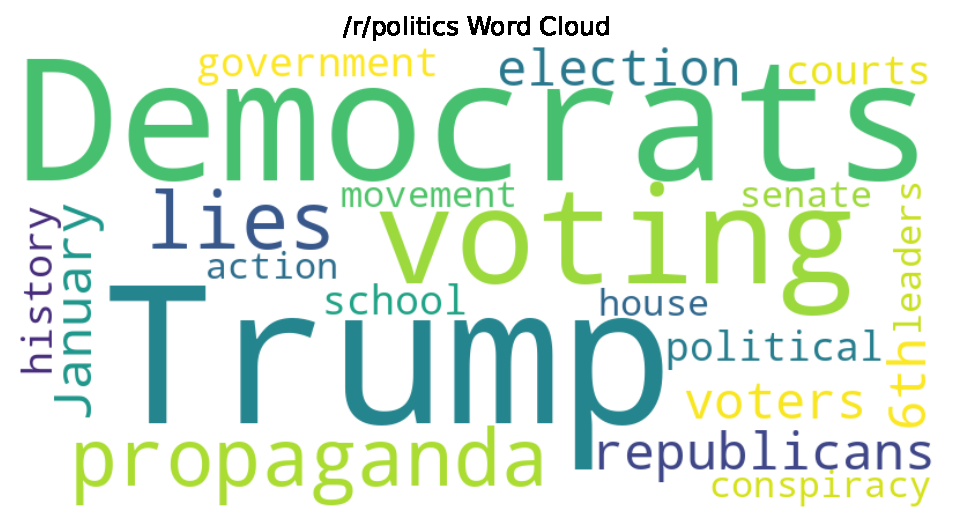
\includegraphics[keepaspectratio]{detecting_bots_on_reddit_code_files/figure-pdf/cell-29-output-2.pdf}}

\pandocbounded{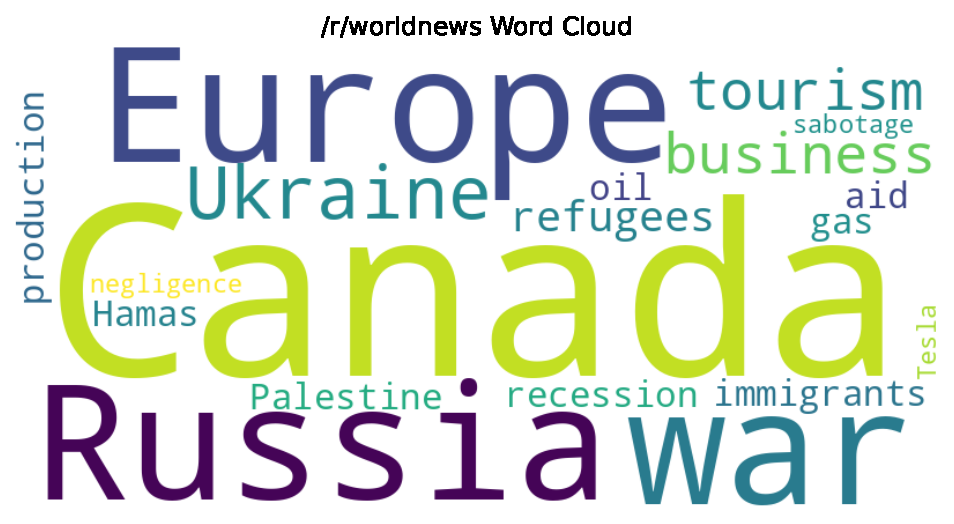
\includegraphics[keepaspectratio]{detecting_bots_on_reddit_code_files/figure-pdf/cell-29-output-3.pdf}}

\pandocbounded{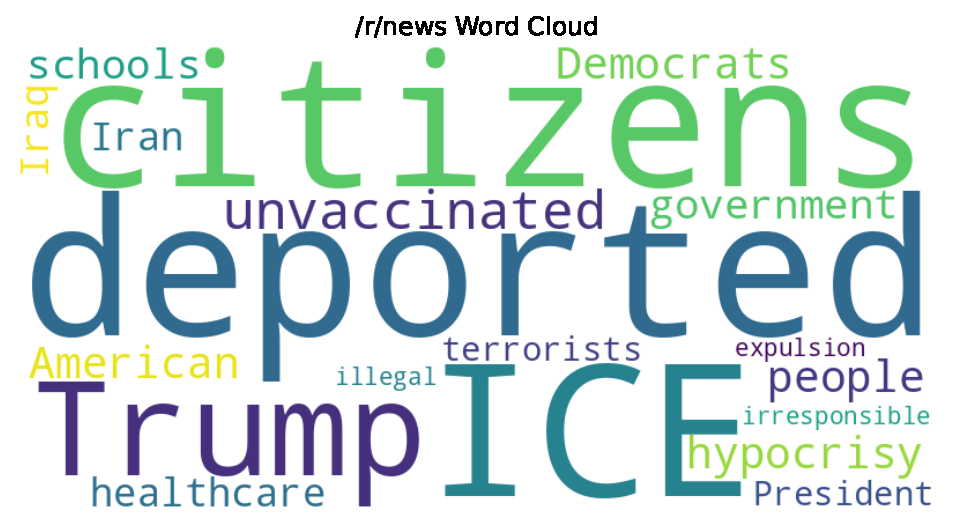
\includegraphics[keepaspectratio]{detecting_bots_on_reddit_code_files/figure-pdf/cell-29-output-4.pdf}}

\pandocbounded{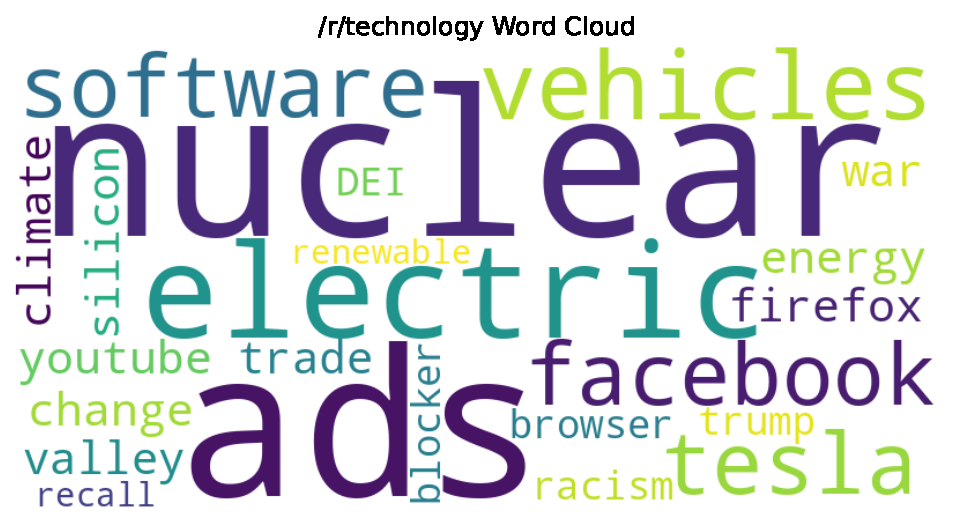
\includegraphics[keepaspectratio]{detecting_bots_on_reddit_code_files/figure-pdf/cell-29-output-5.pdf}}

\pandocbounded{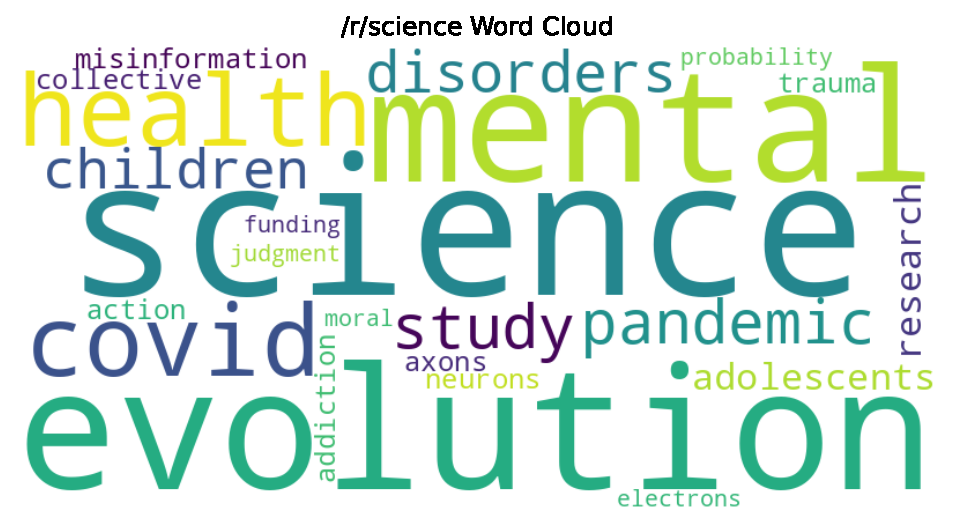
\includegraphics[keepaspectratio]{detecting_bots_on_reddit_code_files/figure-pdf/cell-29-output-6.pdf}}




\end{document}
